\documentclass[11pt,a4paper,oneside]{report}
\usepackage{fontspec}
\setmainfont[Path=fonts/,FontIndex=7,BoldFont=AvenirNext.ttc,BoldFeatures={FontIndex=2},ItalicFont=AvenirNext.ttc,ItalicFeatures={FontIndex=4},BoldItalicFont=AvenirNext.ttc,BoldItalicFeatures={FontIndex=3}]{AvenirNext.ttc}
\setsansfont[Path=fonts/,FontIndex=7,BoldFont=AvenirNext.ttc,BoldFeatures={FontIndex=2},ItalicFont=AvenirNext.ttc,ItalicFeatures={FontIndex=4},BoldItalicFont=AvenirNext.ttc,BoldItalicFeatures={FontIndex=3}]{AvenirNext.ttc}
\newfontfamily\heavy[Path=fonts/,FontIndex=2]{AvenirNext.ttc}
\setmonofont[Path=fonts/,BoldFont=JetBrainsMono-Bold.ttf,ItalicFont=JetBrainsMono-Italic.ttf,Contextuals=NoAlternate,Ligatures=NoCommon]{JetBrainsMono-Regular.ttf}
\usepackage{xcolor,graphicx,tikz,booktabs,tabularx,listings,amsmath}
\usetikzlibrary{arrows.meta,positioning}
\definecolor{paper}{HTML}{FFFFFF}
\definecolor{ink}{HTML}{252525}
\definecolor{teal}{HTML}{252525}
\definecolor{orange}{HTML}{777777}
\definecolor{wash}{HTML}{EAEAEA}
\definecolor{quiet}{HTML}{666666}
\definecolor{lightink}{HTML}{D0D0D0}
\definecolor{codepaper}{HTML}{F6F6F4}
\lstset{language=Python,basicstyle=\ttfamily\fontsize{9.5}{13}\selectfont\color{ink},keywordstyle=\bfseries\color{ink},commentstyle=\itshape\color{quiet},stringstyle=\color{ink},showstringspaces=false,columns=fullflexible,keepspaces=true,breaklines=true,breakatwhitespace=true,numbers=none,upquote=true,aboveskip=8pt,belowskip=6pt}
\hyphenpenalty=4000
\emergencystretch=3em
% The same two-line navigation and fine rule as the reference, without a candy motif.
\newcommand{\guideheader}[2]{\begin{tikzpicture}[remember picture,overlay]
\node[anchor=north west,inner sep=0,text width=176mm] at ([xshift=16mm,yshift=-7mm]current page.north west) {\fontsize{8.5}{10}\selectfont\color{quiet}#1};
\node[anchor=north west,inner sep=0,text width=176mm] at ([xshift=16mm,yshift=-11.5mm]current page.north west) {\heavy\fontsize{10}{12}\selectfont\color{ink}#2};
\draw[lightink,line width=.4pt] ([xshift=16mm,yshift=-17mm]current page.north west)--([xshift=192mm,yshift=-17mm]current page.north west);
\end{tikzpicture}}

\usepackage[a4paper,left=16mm,top=23mm,bottom=19mm,textwidth=132mm,marginparsep=7mm,marginparwidth=37mm,headheight=14pt]{geometry}
\usepackage{fancyhdr,enumitem,hyperref,titlesec,needspace,microtype}
\usepackage[most]{tcolorbox}
\hypersetup{colorlinks=true,linkcolor=ink,urlcolor=ink,bookmarksnumbered=true,pdfauthor={fifteen02}}
\setlength{\parindent}{0pt}\setlength{\parskip}{4pt}
\setlist{nosep,leftmargin=1.4em}
\setcounter{tocdepth}{1}
\titleclass{\chapter}{straight}
\titleformat{\chapter}[display]{\heavy\color{ink}\raggedright}{\fontsize{9}{12}\selectfont\color{quiet}SECTION \thechapter}{5pt}{\fontsize{19}{23}\selectfont}
\titlespacing*{\chapter}{0pt}{14pt}{12pt}
\titleformat{\section}{\heavy\fontsize{12}{15}\selectfont\color{ink}\raggedright}{\thesection}{7pt}{}
\titlespacing*{\section}{0pt}{12pt}{4pt}
\titleformat{\subsection}{\heavy\fontsize{11}{14}\selectfont\raggedright}{}{0pt}{}
\titlespacing*{\subsection}{0pt}{9pt}{3pt}
\pagestyle{fancy}\fancyhf{}
\renewcommand{\chaptermark}[1]{\markboth{#1}{}}
\fancyhead[C]{\guideheader{\lessonheading}{\nouppercase{\leftmark}}}
\fancyfoot[L]{\fontsize{8}{10}\selectfont\color{quiet}Teacher Book\ifnum\lessonnumber>0\relax\quad /\quad Lesson \lessonnumber\fi}
\fancyfoot[R]{\fontsize{9}{11}\selectfont\color{quiet}\thepage}
\fancyhfoffset[R]{44mm}
\renewcommand{\headrulewidth}{0pt}\renewcommand{\footrulewidth}{0pt}
\fancypagestyle{plain}{\fancyhf{}\fancyhead[C]{\guideheader{\lessonheading}{\nouppercase{\leftmark}}}\fancyfoot[L]{\fontsize{8}{10}\selectfont\color{quiet}Teacher Book\ifnum\lessonnumber>0\relax\quad /\quad Lesson \lessonnumber\fi}\fancyfoot[R]{\fontsize{9}{11}\selectfont\color{quiet}\thepage}\renewcommand{\headrulewidth}{0pt}}
\newcommand{\classref}[1]{\marginpar{\raggedright\fontsize{9}{12}\selectfont\color{quiet}\colorbox{wash}{\heavy\fontsize{8}{10}\selectfont IN THE CLASSROOM}\par\smallskip#1}}
\newcommand{\readinggoal}[1]{\par\textbf{What we want to understand.} #1\par\smallskip}
\newcommand{\sectiongoal}[1]{\par{\color{quiet}\textbf{Objective.} #1}\par\smallskip}
\newcommand{\nextpointer}[1]{\par\smallskip{\color{quiet}\textbf{Next.} #1}\par}
\newcommand{\picturecaption}[1]{\par{\small\color{quiet}#1}\par\medskip}
\newtcolorbox{pythonnote}[1]{enhanced,colback=codepaper,colframe=codepaper,boxrule=0pt,sharp corners,borderline west={2.5pt}{0pt}{quiet},left=8pt,right=8pt,top=4pt,bottom=4pt,before skip=6pt,after skip=8pt,fontupper=\small\raggedright,title={PYTHON · #1},fonttitle=\heavy\fontsize{8}{10}\selectfont,coltitle=quiet,colbacktitle=codepaper,attach title to upper={\par\smallskip}}
\newtcolorbox{problembox}[1]{enhanced,colback=white,colframe=ink,boxrule=.6pt,arc=0pt,left=8pt,right=8pt,top=6pt,bottom=6pt,before skip=8pt,after skip=10pt,fontupper=\small,before upper={\raggedright},title={THE PROBLEM · #1},fonttitle=\heavy\fontsize{9}{11}\selectfont,coltitle=white,colbacktitle=ink}
\newtcolorbox{mainidea}{enhanced,colback=wash,colframe=wash,boxrule=0pt,sharp corners,left=10pt,right=10pt,top=8pt,bottom=8pt,before skip=6pt,after skip=10pt,before upper={\raggedright}}
\newtcblisting{bookcode}[1]{enhanced,unbreakable,listing only,listing engine=listings,colback=codepaper,frame hidden,boxrule=0pt,sharp corners,borderline west={2.5pt}{0pt}{ink!88},grow to left by=5mm,grow to right by=44mm,boxsep=0pt,left=26pt,right=12pt,top=6pt,bottom=6pt,before skip=8pt,after skip=8pt,colbacktitle=ink!88,coltitle=white,fonttitle=\heavy\fontsize{10}{13}\selectfont,titlerule=0pt,toptitle=5pt,bottomtitle=5pt,lefttitle=26pt,righttitle=12pt,title={#1\hfill{\ttfamily\fontsize{8}{10}\selectfont\color{white!60!ink}python}},listing options={language=Python,basicstyle=\ttfamily\fontsize{9.5}{13}\selectfont,breaklines=true,breakatwhitespace=true,columns=fullflexible,keepspaces=true,numbers=left,numberstyle=\ttfamily\fontsize{7.5}{13}\selectfont\color{lightink},numbersep=10pt}}
\renewcommand{\thechapter}{\lessonnumber.\arabic{chapter}}\renewcommand{\theHchapter}{\lessonnumber.\arabic{chapter}}
\newcommand{\lessonnumber}{0}\newcommand{\lessonheading}{Teacher Book}\hypersetup{pdftitle={Dynamic Programming: From Recursion to Efficient Solutions - Teacher Book},pdfauthor={fifteen02},bookmarksopen=true}
\fancyfoot[R]{\heavy\fontsize{10}{12}\selectfont\color{ink}\thepage}
\widowpenalty=10000\clubpenalty=10000\displaywidowpenalty=10000
\begin{document}\color{ink}\fontsize{10.5}{13}\selectfont
\thispagestyle{empty}\null
\begin{tikzpicture}[remember picture,overlay]
\node[anchor=north west,inner sep=0,text width=174mm] at ([xshift=18mm,yshift=-24mm]current page.north west) {\heavy\fontsize{43}{47}\selectfont\raggedright Dynamic\\Programming};
\node[anchor=north west,inner sep=0,text width=174mm] at ([xshift=18mm,yshift=-68mm]current page.north west) {\fontsize{19}{25}\selectfont\raggedright From Recursion to Efficient Solutions};
\node[anchor=north west,inner sep=0,text width=174mm] at ([xshift=18mm,yshift=-94mm]current page.north west) {\heavy\fontsize{15}{19}\selectfont Teacher Book\quad {\normalfont\color{quiet}Lessons 1–5}};
\node[anchor=north west,inner sep=0,text width=174mm] at ([xshift=18mm,yshift=-107mm]current page.north west) {\fontsize{12}{16}\selectfont\raggedright Prepare the reasoning, work through the examples,\\and understand the complete solutions.};
\node[anchor=center,inner sep=0] at ([xshift=105mm,yshift=-166mm]current page.north west) {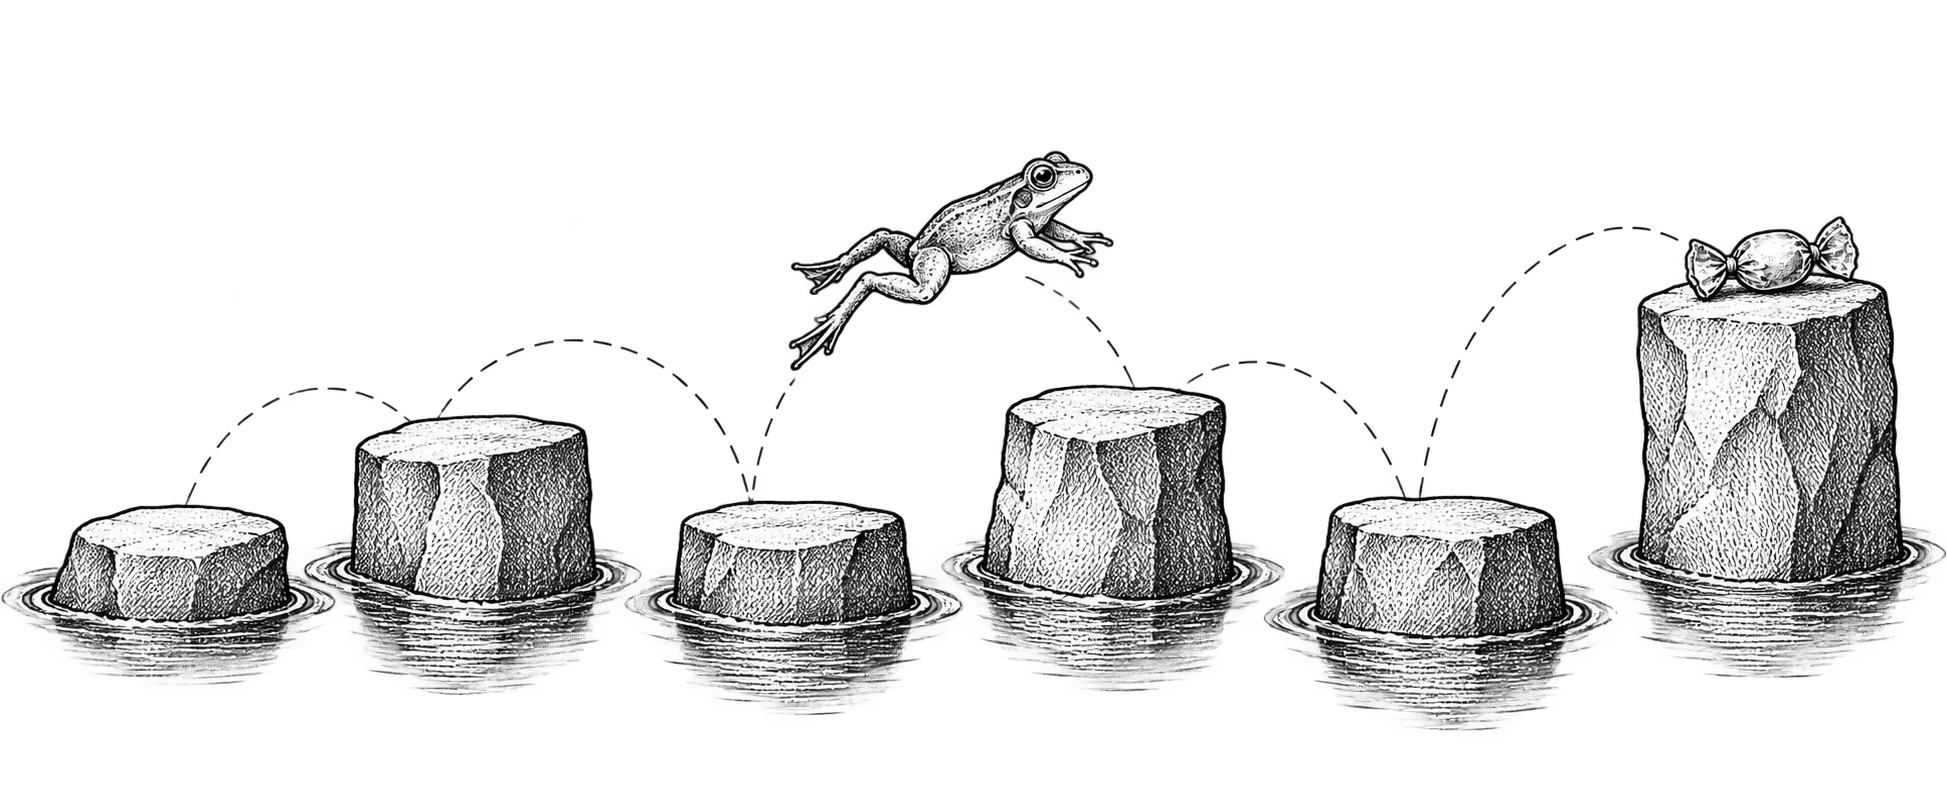
\includegraphics[width=174mm,height=88mm,keepaspectratio]{assets/cover.png}};
\node[anchor=north west,inner sep=0,text width=174mm] at ([xshift=18mm,yshift=-226mm]current page.north west) {\fontsize{12}{16}\selectfont Staircase and Frog · Dice and Grid Paths\\Tower and Array Description · Fruit Feast\\Hoof, Paper, Scissors};
\node[anchor=west,inner sep=0] at ([xshift=18mm,yshift=-269mm]current page.north west) {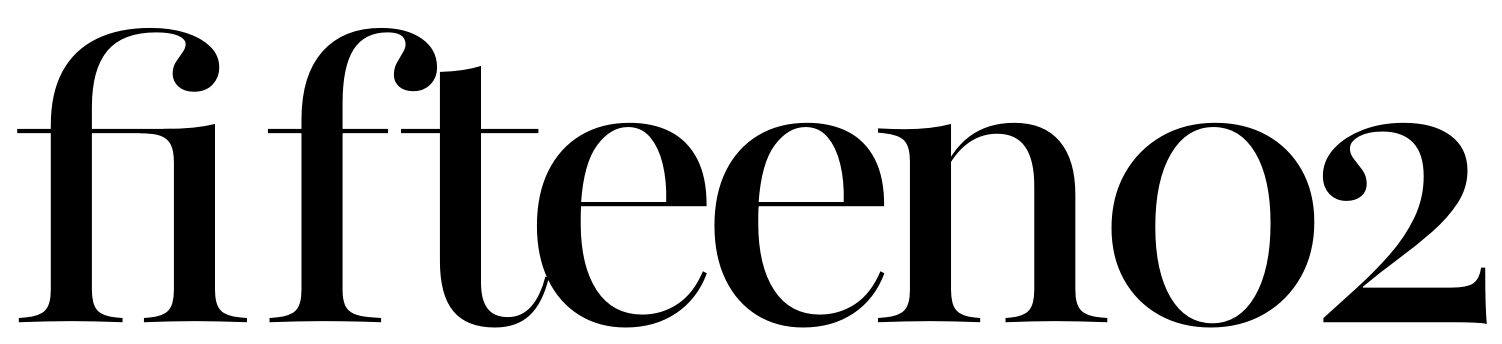
\includegraphics[width=43mm]{assets/logo.png}};
\node[anchor=east,inner sep=0] at ([xshift=192mm,yshift=-269mm]current page.north west) {
\includegraphics[width=62mm]{assets/julians-pathfinder-monochrome.pdf}};
\end{tikzpicture}\clearpage
\markboth{Contents}{}\pdfbookmark[0]{Contents}{contents}\noindent\makebox[\linewidth][l]{\begin{minipage}{176mm}{\heavy\fontsize{28}{33}\selectfont Contents\par}\vspace{5mm}
\begin{minipage}{140mm}\raggedright Read the relevant lesson before class. Each lesson develops the ideas through worked examples, diagrams, complete programs and explanations of their running time. Margin notes identify the matching classroom questions.\end{minipage}\par\vspace{7mm}
\noindent\begin{minipage}[t][29mm][t]{176mm}\vspace{0pt}{\color{lightink}\hrule height .35pt}\vspace{5mm}\begin{minipage}[t]{18mm}\vspace{0pt}{\heavy\fontsize{26}{29}\selectfont 1}\end{minipage}\begin{minipage}[t]{140mm}\vspace{0pt}{\heavy\fontsize{14}{18}\selectfont\hyperref[lesson-1]{Staircase and Frog}\par}\vspace{2mm}{\color{quiet}Remember the answer.}\end{minipage}\begin{minipage}[t]{18mm}\vspace{0pt}\raggedleft{\heavy\fontsize{14}{18}\selectfont\pageref{lesson-1}}\end{minipage}\end{minipage}\par
\noindent\begin{minipage}[t][29mm][t]{176mm}\vspace{0pt}{\color{lightink}\hrule height .35pt}\vspace{5mm}\begin{minipage}[t]{18mm}\vspace{0pt}{\heavy\fontsize{26}{29}\selectfont 2}\end{minipage}\begin{minipage}[t]{140mm}\vspace{0pt}{\heavy\fontsize{14}{18}\selectfont\hyperref[lesson-2]{Dice Combinations and Grid Paths}\par}\vspace{2mm}{\color{quiet}Count the ways to arrive.}\end{minipage}\begin{minipage}[t]{18mm}\vspace{0pt}\raggedleft{\heavy\fontsize{14}{18}\selectfont\pageref{lesson-2}}\end{minipage}\end{minipage}\par
\noindent\begin{minipage}[t][29mm][t]{176mm}\vspace{0pt}{\color{lightink}\hrule height .35pt}\vspace{5mm}\begin{minipage}[t]{18mm}\vspace{0pt}{\heavy\fontsize{26}{29}\selectfont 3}\end{minipage}\begin{minipage}[t]{140mm}\vspace{0pt}{\heavy\fontsize{14}{18}\selectfont\hyperref[lesson-3]{Mortal Kombat Tower and Array Description}\par}\vspace{2mm}{\color{quiet}Remember the missing detail.}\end{minipage}\begin{minipage}[t]{18mm}\vspace{0pt}\raggedleft{\heavy\fontsize{14}{18}\selectfont\pageref{lesson-3}}\end{minipage}\end{minipage}\par
\noindent\begin{minipage}[t][29mm][t]{176mm}\vspace{0pt}{\color{lightink}\hrule height .35pt}\vspace{5mm}\begin{minipage}[t]{18mm}\vspace{0pt}{\heavy\fontsize{26}{29}\selectfont 4}\end{minipage}\begin{minipage}[t]{140mm}\vspace{0pt}{\heavy\fontsize{14}{18}\selectfont\hyperref[lesson-4]{Fruit Feast}\par}\vspace{2mm}{\color{quiet}Track what is possible.}\end{minipage}\begin{minipage}[t]{18mm}\vspace{0pt}\raggedleft{\heavy\fontsize{14}{18}\selectfont\pageref{lesson-4}}\end{minipage}\end{minipage}\par
\noindent\begin{minipage}[t][29mm][t]{176mm}\vspace{0pt}{\color{lightink}\hrule height .35pt}\vspace{5mm}\begin{minipage}[t]{18mm}\vspace{0pt}{\heavy\fontsize{26}{29}\selectfont 5}\end{minipage}\begin{minipage}[t]{140mm}\vspace{0pt}{\heavy\fontsize{14}{18}\selectfont\hyperref[lesson-5]{Hoof, Paper, Scissors}\par}\vspace{2mm}{\color{quiet}Choose when to switch.}\end{minipage}\begin{minipage}[t]{18mm}\vspace{0pt}\raggedleft{\heavy\fontsize{14}{18}\selectfont\pageref{lesson-5}}\end{minipage}\end{minipage}\par
\vspace{5mm}\begin{minipage}{140mm}\raggedright\textbf{Using the two books}\par Teacher Book is for preparation. Teacher Class Notes is for teaching. Question IDs such as L1-04 match the worksheets, slides and notebooks. Each lesson folder holds the classroom materials and practice files.\end{minipage}\end{minipage}}
\clearpage\renewcommand{\lessonnumber}{1}\renewcommand{\lessonheading}{Lesson 1 · Staircase and Frog}\setcounter{chapter}{0}\setcounter{section}{0}\phantomsection\label{lesson-1}\pdfbookmark[-1]{Lesson 1: Staircase and Frog}{lesson-1-bookmark}
\noindent\makebox[\linewidth][l]{\begin{minipage}{176mm}{\heavy\fontsize{23}{28}\selectfont\raggedright Lesson 1\par}\vspace{2mm}{\heavy\fontsize{19}{24}\selectfont\raggedright Staircase and Frog\par}\end{minipage}}\par\vspace{5mm}
\markboth{The lesson route}{}
\begin{mainidea}{\color{quiet}\heavy\fontsize{9}{11}\selectfont MAIN IDEA OF LESSON 1}\par\smallskip{\heavy\fontsize{17}{21}\selectfont Remember the answer.}\par\smallskip Remember the answer to each question so that it is never worked out twice, and then choose an order in which every answer you need is already known.\end{mainidea}
We first trace functions that call themselves, learn how they stop, and write a small recursive function. Then we count routes up a staircase. The first program follows every choice, so we can see why its answer is correct. We then notice that many calls ask the same question. Saving their answers removes repeated work; filling a table in order also removes the deep call stack. Frog uses the same sequence of ideas, but its stored answers are costs rather than counts, so one problem adds answers and the other takes a minimum.

\textbf{After this lesson you will be able to}\begin{itemize}\item state each problem exactly and solve small cases by hand;\item explain a recurrence from the last move, including its starting values;\item count the calls of a slow recursion and point to the line that causes them;\item cache answers in a dictionary and explain why the call stack is still deep;\item fill a table with a loop, give its cost line by line, and submit Frog to AtCoder.\end{itemize}
\Needspace{6\baselineskip}\textbf{The route}\par
\textbf{1. Recursion: follow one smaller call.} Read a function that calls itself, see how it stops, then write one before trying staircase.\par
\textbf{2. Staircase: start with routes we can see.} Understand the staircase problem and why its answer is a sum, before writing any code.\par
\textbf{3. Remember an answer, then choose the order.} Remove repeated computation with a cache, then remove deep recursion with a loop.\par
\textbf{4. Frog: keep the cheapest route.} Reuse the same ideas when the stored answers are costs, combined with min instead of +.\par
\textbf{5. Run, test and explain your program.} Use the starter file, the test files and the runner; read every edge file.\par
Read this lesson before class. Teacher Class Notes holds the short classroom prompts and answers; the margin notes here name the matching question IDs on the worksheet, slides and notebook. Every program is printed in full, and every number about running code (call counts, line counts, wrong outputs) was produced by running the programs.

Students need Python functions, lists, loops, indexing, comparisons and basic arithmetic. Each new Python feature is explained in a grey PYTHON note beside the first program that uses it.

Each section opens with its objective and ends by pointing to the next. Each problem ends with its edge cases, common mistakes (with the wrong output each one produces), how to submit it and a recap. The summary tables and the two-hour plan are in the appendix.


\Needspace{22\baselineskip}
\chapter{Recursion: follow one smaller call}
\readinggoal{Read a function that calls itself, see how it stops, then write one before trying staircase.}
\Needspace{21\baselineskip}
\section{A function can call itself}
\classref{L1-01}
\sectiongoal{Follow each call and distinguish printing a line from returning a value.}
We begin with a countdown. The input is the nonnegative integer n. For the worked example, n is 3. A new call receives its own value of n; it does not change the input held by the call that made it.

\Needspace{16\baselineskip}\begin{problembox}{Countdown}\textbf{Story.} Print a countdown before starting an activity.\par\smallskip \textbf{Rules.} Print each integer from n down to 1, one per line, then print Go! once. For n = 0, print only Go!.\par\smallskip \textbf{Input.} A nonnegative integer n, supplied as a function argument.\par\smallskip \textbf{Output.} The printed countdown.\par\smallskip \textbf{Limits.} Use n from 0 to 5 for these hand traces.\par\smallskip \textbf{Example input.}
\begin{lstlisting}[language={},aboveskip=2pt,belowskip=2pt]
countdown(3)
\end{lstlisting}
\textbf{Expected output:} 3, then 2, then 1, then Go! (separate lines)\par\smallskip The table below follows the actual print order.\par\smallskip\textbf{Source.} original teaching exercise.\end{problembox}
A function calling itself is called recursion. In the listing, countdown(n - 1) makes a new call with an input one smaller. The current call pauses until that call has finished.

\Needspace{12\baselineskip}
\begin{bookcode}{countdown}
def countdown(n):
    if n == 0:
        print('Go!')
        return
    print(n)
    countdown(n - 1)
\end{bookcode}
\Needspace{6\baselineskip}\begin{pythonnote}{print and return}\texttt{def countdown(n):} names the function and its input. \texttt{print} writes a line on screen; it does not finish the function. \texttt{return} finishes the current call immediately. Here the bare \texttt{return} gives no numerical answer. The indented lines under \texttt{if n == 0:} run only for that input.\end{pythonnote}
\Needspace{7\baselineskip}
\par\medskip\begingroup\small\setlength{\tabcolsep}{4pt}\renewcommand{\arraystretch}{1.3}\begin{tabularx}{\linewidth}{>{\raggedright\arraybackslash}X>{\raggedright\arraybackslash}X>{\raggedright\arraybackslash}X}\toprule\textbf{Call} & \textbf{Prints} & \textbf{Next call}\\\midrule
{}countdown(3) & 3 & countdown(2)\\
{}countdown(2) & 2 & countdown(1)\\
{}countdown(1) & 1 & countdown(0)\\
{}countdown(0) & Go! & no new call\\
\bottomrule\end{tabularx}\endgroup\par\medskip
The base case is the input answered without another recursive call. Here it is n = 0. Every other call reduces a positive n by 1, so it eventually reaches that base case. L1-01 asks students to reconstruct this trace.

\nextpointer{Use a stopping case to end the chain of calls.}
\Needspace{17\baselineskip}
\section{A call waits for a returned value}
\classref{L1-02}
\sectiongoal{Follow the waiting calls and calculate their answers from the base case upward.}
Now sum\_to(n) returns the sum of the integers from 1 through n. For n = 0 it returns 0. Our example is sum\_to(3). Unlike countdown, this function returns a number; it does not print the intermediate numbers.

\Needspace{12\baselineskip}
\begin{bookcode}{sum to}
def sum_to(n):
    if n == 0:
        return 0
    return n + sum_to(n - 1)
\end{bookcode}
The expression n + sum\_to(n - 1) cannot finish its addition until the smaller call returns. Python keeps unfinished calls on the call stack: the newest call is on top, with the calls waiting for it underneath.

\Needspace{12\baselineskip}\begin{center}\begin{tikzpicture}[x=1cm,y=1cm,>=Stealth]
\node[anchor=west,font=\small] at (-2.5,3.1) {Newest call: answers first};
\node[draw,fill=wash,minimum width=4.7cm,minimum height=.7cm] at (0,2.4) {sum\_to(0): returns 0};
\node[draw,minimum width=4.7cm,minimum height=.7cm] at (0,1.5) {sum\_to(1): waits};
\node[draw,minimum width=4.7cm,minimum height=.7cm] at (0,.6) {sum\_to(2): waits};
\node[draw,minimum width=4.7cm,minimum height=.7cm] at (0,-.3) {sum\_to(3): waits};
\draw[->,thick] (2.8,2.4)--node[right,font=\small,align=left]{Values return\\to waiting calls}(2.8,-.3);
\end{tikzpicture}\end{center}\picturecaption{The stack after sum\_to(3) has called down to sum\_to(0). The top call can answer directly; the other three are waiting.}
Calls enter the table from top to bottom. Evaluate the Returns column from bottom to top, using the result of the row below.

\Needspace{7\baselineskip}
\par\medskip\begingroup\small\setlength{\tabcolsep}{4pt}\renewcommand{\arraystretch}{1.3}\begin{tabularx}{\linewidth}{>{\raggedright\arraybackslash}X>{\raggedright\arraybackslash}X>{\raggedright\arraybackslash}X}\toprule\textbf{Call} & \textbf{Waits for} & \textbf{Returns}\\\midrule
{}sum\_to(3) & sum\_to(2) & 3 + 3 = 6\\
{}sum\_to(2) & sum\_to(1) & 2 + 1 = 3\\
{}sum\_to(1) & sum\_to(0) & 1 + 0 = 1\\
{}sum\_to(0) & nothing (base case) & 0\\
\bottomrule\end{tabularx}\endgroup\par\medskip
For L1-02, sum\_squares(n) returns the sum of the squares from 1 through n. The data is n = 4. Each waiting call adds n * n, rather than n.

\Needspace{12\baselineskip}
\begin{bookcode}{sum squares}
def sum_squares(n):
    if n == 0:
        return 0
    return n * n + sum_squares(n - 1)
\end{bookcode}
\Needspace{8\baselineskip}
\par\medskip\begingroup\small\setlength{\tabcolsep}{4pt}\renewcommand{\arraystretch}{1.3}\begin{tabularx}{\linewidth}{>{\raggedright\arraybackslash}X>{\raggedright\arraybackslash}X>{\raggedright\arraybackslash}X}\toprule\textbf{Call} & \textbf{Waits for} & \textbf{Returns}\\\midrule
{}sum\_squares(4) & sum\_squares(3) & 16 + 14 = 30\\
{}sum\_squares(3) & sum\_squares(2) & 9 + 5 = 14\\
{}sum\_squares(2) & sum\_squares(1) & 4 + 1 = 5\\
{}sum\_squares(1) & sum\_squares(0) & 1 + 0 = 1\\
{}sum\_squares(0) & nothing & 0\\
\bottomrule\end{tabularx}\endgroup\par\medskip
\nextpointer{Repair a function whose calls never reach a stopping case.}
\Needspace{16\baselineskip}
\section{Find and repair the missing base case}
\classref{L1-03}
\sectiongoal{Identify why calls continue past the intended stopping input.}
power2(n) should return 2 raised to the nonnegative integer n. For example, the data n = 3 means multiplying three copies of 2. The worksheet supplies this deliberately incomplete function. Trace it on paper before running it.

\Needspace{5\baselineskip}
\begin{lstlisting}[language={}]
def power2(n):
    return 2 * power2(n - 1)
\end{lstlisting}
\Needspace{8\baselineskip}
\par\medskip\begingroup\small\setlength{\tabcolsep}{4pt}\renewcommand{\arraystretch}{1.3}\begin{tabularx}{\linewidth}{>{\raggedright\arraybackslash}X>{\raggedright\arraybackslash}X>{\raggedright\arraybackslash}X}\toprule\textbf{Call number} & \textbf{Input n} & \textbf{Next input}\\\midrule
{}1 & 3 & 2\\
{}2 & 2 & 1\\
{}3 & 1 & 0\\
{}4 & 0 & -1\\
{}5 & -1 & -2\\
\bottomrule\end{tabularx}\endgroup\par\medskip
No call answers directly, so the input passes 0 and keeps decreasing. Python eventually raises RecursionError when too many calls are unfinished. The exact failing depth varies. The repair needs a stopping case before the recursive call. By definition, 2 raised to 0 is 1.

\Needspace{12\baselineskip}
\begin{bookcode}{power2}
def power2(n):
    if n == 0:
        return 1
    return 2 * power2(n - 1)
\end{bookcode}
\Needspace{7\baselineskip}
\par\medskip\begingroup\small\setlength{\tabcolsep}{4pt}\renewcommand{\arraystretch}{1.3}\begin{tabularx}{\linewidth}{>{\raggedright\arraybackslash}X>{\raggedright\arraybackslash}X>{\raggedright\arraybackslash}X}\toprule\textbf{Call} & \textbf{Waits for} & \textbf{Returns}\\\midrule
{}power2(3) & power2(2) & 2 x 4 = 8\\
{}power2(2) & power2(1) & 2 x 2 = 4\\
{}power2(1) & power2(0) & 2 x 1 = 2\\
{}power2(0) & nothing & 1\\
\bottomrule\end{tabularx}\endgroup\par\medskip
\nextpointer{Write a recursive function from a stated rule.}
\Needspace{17\baselineskip}
\section{Write one small recursive function}
\classref{L1-04}
\sectiongoal{Write factorial using a directly known answer and one smaller call.}
The factorial of n is the product of the integers from 1 through n; factorial(0) is defined as 1. Use nonnegative integers. Ask students to write the function before showing this solution. The worked example uses n = 4.

\Needspace{12\baselineskip}
\begin{bookcode}{factorial}
def factorial(n):
    if n == 0:
        return 1
    return n * factorial(n - 1)
\end{bookcode}
\Needspace{8\baselineskip}
\par\medskip\begingroup\small\setlength{\tabcolsep}{4pt}\renewcommand{\arraystretch}{1.3}\begin{tabularx}{\linewidth}{>{\raggedright\arraybackslash}X>{\raggedright\arraybackslash}X>{\raggedright\arraybackslash}X}\toprule\textbf{Call} & \textbf{Waits for} & \textbf{Returns}\\\midrule
{}factorial(4) & factorial(3) & 4 x 6 = 24\\
{}factorial(3) & factorial(2) & 3 x 2 = 6\\
{}factorial(2) & factorial(1) & 2 x 1 = 2\\
{}factorial(1) & factorial(0) & 1 x 1 = 1\\
{}factorial(0) & nothing & 1\\
\bottomrule\end{tabularx}\endgroup\par\medskip
\Needspace{10\baselineskip}\textbf{Which lines do the work?}
\Needspace{5\baselineskip}
\par\medskip\begingroup\footnotesize\setlength{\tabcolsep}{4pt}\renewcommand{\arraystretch}{1.3}\begin{tabularx}{\linewidth}{>{\raggedright\arraybackslash}p{8mm}>{\raggedright\arraybackslash}p{40mm}>{\raggedright\arraybackslash}X>{\raggedright\arraybackslash}p{17mm}>{\raggedright\arraybackslash}p{20mm}}\toprule\textbf{Line} & \textbf{Code} & \textbf{How often it runs} & \textbf{n = 4} & \textbf{n = 10}\\\midrule
{}2 & \texttt{if n == 0:} & once for every call, including the base case & 5 & 11\\
{}4 & \texttt{return n * factorial(n - 1)} & once for each positive input & 4 & 10\\
\bottomrule\end{tabularx}\endgroup\par\medskip
There is one smaller call for each positive input. The number of calls and the maximum number of unfinished calls both grow in proportion to n; this is O(n) call work and O(n) stack space. Multiplying large integers takes more work than multiplying small ones, so this counts calls rather than every arithmetic operation.

\Needspace{6\baselineskip}\par\medskip{\heavy Recap}\par\begin{itemize}\item A base case answers without another call.\item Every recursive call must move toward a base case.\item A returned value goes back to the waiting call.\item The staircase will ask two smaller questions instead of one.\end{itemize}
\nextpointer{Try the staircase, where one call will ask two smaller questions.}
\Needspace{22\baselineskip}
\chapter{Staircase: start with routes we can see}
\readinggoal{Understand the staircase problem and why its answer is a sum, before writing any code.}
\Needspace{21\baselineskip}
\section{The staircase problem}
\classref{L1-05}
\sectiongoal{State the problem exactly: what is counted, what the input is and what the answer must be.}
This lesson has one main idea: remember the answer to a question so that it is never worked out twice. We meet it first in a counting problem small enough to do by hand.

\Needspace{16\baselineskip}\begin{problembox}{Staircase}\textbf{Story.} You stand on the ground below a staircase and climb it by single or double steps.\par\smallskip \textbf{Rules.} The ground is step 0. Each move climbs exactly 1 step or exactly 2 steps. A route is the ordered list of moves; [1, 2] and [2, 1] are different routes. Count the routes that land exactly on step n. In the variation (L1-13) the moves are 1 or 3 instead.\par\smallskip \textbf{Input.} One line holding the target step n.\par\smallskip \textbf{Output.} The exact number of routes (no remainder is taken; Python integers have no size limit).\par\smallskip \textbf{Limits.} In our practice files 0 ≤ n ≤ 10,000; the answer for 10,000 has 2,090 digits.\par\smallskip \textbf{Example input.}
\begin{lstlisting}[language={},aboveskip=2pt,belowskip=2pt]
5
\end{lstlisting}
\textbf{Expected output:} 8\par\smallskip The eight routes are 11111, 1112, 1121, 1211, 2111, 122, 212 and 221.\par\smallskip\textbf{Source.} an original teaching exercise for this course; there is no online judge, so students test it with the local files.\end{problembox}
We are counting ordered lists of moves. A route written as [1, 2, 2] visits steps 1, 3 and 5; [2, 1, 2] visits steps 2, 3 and 5. Both finish at step 5, but they are different routes because their moves occur in a different order. To save space we write a route as its digits: 122 means [1, 2, 2].

\nextpointer{List the routes for small targets by hand.}
\Needspace{21\baselineskip}
\section{Five steps, eight routes}
\classref{L1-05}
\sectiongoal{Build the complete list of routes for targets 1 to 5 and notice how the counts grow.}
For the first step there is only 1. For the second there are 11 and 2. For the third there are 111, 12 and 21. Continue drawing before looking for a formula.

\Needspace{8\baselineskip}
\par\medskip\begingroup\small\setlength{\tabcolsep}{4pt}\renewcommand{\arraystretch}{1.3}\begin{tabularx}{\linewidth}{>{\raggedright\arraybackslash}p{20mm}>{\raggedright\arraybackslash}X>{\raggedright\arraybackslash}p{12mm}}\toprule\textbf{Target step} & \textbf{Routes (122 means [1, 2, 2])} & \textbf{Count}\\\midrule
{}1 & 1 & 1\\
{}2 & 11, 2 & 2\\
{}3 & 111, 12, 21 & 3\\
{}4 & 1111, 112, 121, 211, 22 & 5\\
{}5 & 11111, 1112, 1121, 1211, 2111, 122, 212, 221 & 8\\
\bottomrule\end{tabularx}\endgroup\par\medskip
Each digit in the table represents one move. The target step is a position; the number of routes is the answer stored for that position. Step 4 has five routes; the fact that its position is 4 does not make the answer 4.

At the board, let students build the first few rows themselves. The useful question is how to know that a list of routes is complete.

\nextpointer{Find a way to organise the routes so that none is missed or counted twice.}
\Needspace{21\baselineskip}
\section{Look at the final move}
\classref{L1-06}
\sectiongoal{Explain why the count for step 5 is the count for step 4 plus the count for step 3.}
A route reaching step 5 must end with a jump of 1 from step 4 or a jump of 2 from step 3. There is no other possible last move. We already know five routes to step 4. Append a jump of 1 to each of them: that gives five routes to step 5. Likewise, append a jump of 2 to each of the three routes to step 3: that gives three more.

\Needspace{10\baselineskip}
\begin{center}\begin{tikzpicture}[>=Stealth,every node/.style={font=\small},box/.style={draw=teal,rounded corners,minimum width=20mm,minimum height=8mm,fill=wash},arr/.style={->,thick,teal}]\node[box] (a) at (0,1) {step 4};\node[box] (b) at (0,-1) {step 3};\node[box] (c) at (8,0) {step 5};\draw[arr] (a)--node[above,sloped]{5 routes, then jump 1}(c);\draw[arr] (b)--node[below,sloped]{3 routes, then jump 2}(c);\end{tikzpicture}\end{center}These two groups cannot overlap: every route in the first group ends in 1 and every route in the second ends in 2. Together they include every legal route. This is why we add 5 and 3, obtaining 8. The addition follows from a partition of the routes, not just from spotting a pattern in the numbers.

\Needspace{6\baselineskip}
\par\medskip\begingroup\small\setlength{\tabcolsep}{4pt}\renewcommand{\arraystretch}{1.3}\begin{tabularx}{\linewidth}{>{\raggedright\arraybackslash}X>{\raggedright\arraybackslash}X>{\raggedright\arraybackslash}X>{\raggedright\arraybackslash}X}\toprule\textbf{Last move} & \textbf{Earlier step} & \textbf{Routes there} & \textbf{Routes to step 5 in this group}\\\midrule
{}1 & 4 & 5 & 11111, 1121, 1211, 2111, 221\\
{}2 & 3 & 3 & 1112, 122, 212\\
{}Total &  & 5 + 3 = 8 & all eight, each exactly once\\
\bottomrule\end{tabularx}\endgroup\par\medskip
Now name the question. Let ways(n) be the number of routes from the ground to step n. Its argument n identifies the target step; its value counts routes. For a positive target the same last-move reasoning gives ways(n) = ways(n − 1) + ways(n − 2). A rule expressing an answer using answers to smaller questions is called a recurrence. “Smaller” refers to the target step; the recursive calls return route counts, not step numbers.

\nextpointer{Turn the rule into a function and give it somewhere to stop.}
\Needspace{24\baselineskip}
\section{Give the recursion somewhere to stop}
\classref{L1-07\\L1-08}
\sectiongoal{Choose the stopping cases ways(0) = 1 and ways(−1) = 0, then write and trace the first program.}
A function cannot keep asking smaller questions for ever. At step 0 there is exactly one route: make no moves. This empty route is needed when we build a route consisting of one final jump: the one-jump route [2] is the empty route to step 0 followed by 2.

A negative target has no routes because every allowed jump moves upward. Thus ways(0) is 1 and ways(−1) is 0, and the recurrence gives ways(1) = ways(0) + ways(−1) = 1 + 0 = 1.

The first program translates that explanation directly. In code the function is called \texttt{stairs\_slow}; \texttt{stairs\_slow(n)} computes ways(n).

\Needspace{12\baselineskip}
\begin{bookcode}{stairs slow}
def stairs_slow(n):
    if n < 0:
        return 0
    if n == 0:
        return 1
    return stairs_slow(n - 1) + stairs_slow(n - 2)
\end{bookcode}
\Needspace{5\baselineskip}\textbf{Try it.}

\begin{lstlisting}
print(stairs_slow(5))
\end{lstlisting}
\textbf{Result:} 8

\textbf{Recursion depth.} Python stops recursion at about 1,000 nested calls by default, so this recursive version is for small inputs and the small and edge test files only. Use the iterative version for the medium and large files.

\Needspace{6\baselineskip}\begin{pythonnote}{functions that call themselves}\texttt{def stairs\_slow(n):} defines a function with one parameter, n. \texttt{return} hands a value back to whoever called the function and ends the call at once, so line 3 ends the call for a negative n before line 6 is reached. A function may call itself (line 6): each call is a separate question with its own n. Python pauses the calling line until the smaller call returns its number, then continues the addition.\end{pythonnote}
The table traces \texttt{stairs\_slow(3)} in the order Python makes the calls. Each dot of indentation is one level deeper. A call returns its number to the call waiting for it; it does not jump the program straight to the final answer.

\Needspace{12\baselineskip}
\par\medskip\begingroup\small\setlength{\tabcolsep}{4pt}\renewcommand{\arraystretch}{1.3}\begin{tabularx}{\linewidth}{>{\raggedright\arraybackslash}p{10mm}>{\raggedright\arraybackslash}p{36mm}>{\raggedright\arraybackslash}X>{\raggedright\arraybackslash}p{14mm}}\toprule\textbf{Order} & \textbf{Call} & \textbf{What it asks} & \textbf{Returns}\\\midrule
{}1 & stairs\_slow(3) & stairs\_slow(2) + stairs\_slow(1) = 2 + 1 & 3\\
{}2 & . stairs\_slow(2) & stairs\_slow(1) + stairs\_slow(0) = 1 + 1 & 2\\
{}3 & . . stairs\_slow(1) & stairs\_slow(0) + stairs\_slow(-1) = 1 + 0 & 1\\
{}4 & . . . stairs\_slow(0) & nothing: k = 0 & 1\\
{}5 & . . . stairs\_slow(-1) & nothing: k < 0 & 0\\
{}6 & . . stairs\_slow(0) & nothing: k = 0 & 1\\
{}7 & . stairs\_slow(1) & stairs\_slow(0) + stairs\_slow(-1) = 1 + 0 & 1\\
{}8 & . . stairs\_slow(0) & nothing: k = 0 & 1\\
{}9 & . . stairs\_slow(-1) & nothing: k < 0 & 0\\
\bottomrule\end{tabularx}\endgroup\par\medskip
Notice that \texttt{stairs\_slow(1)} is computed twice (calls 3 and 7) and \texttt{stairs\_slow(0)} three times. That waste is the subject of the next chapter.

\nextpointer{Count how many calls this program makes, and why.}
\Needspace{22\baselineskip}
\chapter{Remember an answer, then choose the order}
\readinggoal{Remove repeated computation with a cache, then remove deep recursion with a loop.}
\Needspace{23\baselineskip}
\section{A tree contains repeated questions}
\classref{L1-09}
\sectiongoal{See, and count, the repeated calls that make the first program slow.}
The call for target 5 asks about targets 4 and 3. The call for target 4 also asks about target 3. Those two calls for target 3 have exactly the same meaning: count routes from the ground to step 3 under the same rules. Repeating the calculation cannot change its answer. The picture shows every call that \texttt{stairs\_slow(5)} makes.

\Needspace{12\baselineskip}\begin{center}\begin{tikzpicture}[>=Stealth,every node/.style={font=\small},box/.style={draw=ink,rounded corners=2pt,minimum height=7mm,fill=paper,inner sep=3pt},arr/.style={->,thick,ink},thin arr/.style={->,ink},call/.style={circle,draw=ink,minimum size=6.4mm,inner sep=0pt,font=\ttfamily\footnotesize},repeat/.style={call,fill=wash,draw=quiet,dashed},cell/.style={draw=ink,minimum size=9mm,inner sep=0pt},note/.style={font=\footnotesize,text=quiet},scale=0.92,every node/.append style={transform shape}]\node[call] (n0) at (7.20,0.00) {5};\node[call] (n1) at (4.23,-1.05) {4};\node[call] (n2) at (2.33,-2.10) {3};\node[call] (n3) at (1.23,-3.15) {2};\node[call] (n4) at (0.49,-4.20) {1};\node[call] (n5) at (0.00,-5.25) {0};\node[call] (n6) at (0.98,-5.25) {-1};\node[repeat] (n7) at (1.96,-4.20) {0};\node[repeat] (n8) at (3.43,-3.15) {1};\node[repeat] (n9) at (2.94,-4.20) {0};\node[repeat] (n10) at (3.92,-4.20) {-1};\node[repeat] (n11) at (6.12,-2.10) {2};\node[repeat] (n12) at (5.39,-3.15) {1};\node[repeat] (n13) at (4.90,-4.20) {0};\node[repeat] (n14) at (5.88,-4.20) {-1};\node[repeat] (n15) at (6.86,-3.15) {0};\node[repeat] (n16) at (10.17,-1.05) {3};\node[repeat] (n17) at (9.06,-2.10) {2};\node[repeat] (n18) at (8.33,-3.15) {1};\node[repeat] (n19) at (7.84,-4.20) {0};\node[repeat] (n20) at (8.82,-4.20) {-1};\node[repeat] (n21) at (9.80,-3.15) {0};\node[repeat] (n22) at (11.27,-2.10) {1};\node[repeat] (n23) at (10.78,-3.15) {0};\node[repeat] (n24) at (11.76,-3.15) {-1};\draw[ink] (n4)--(n5);\draw[ink] (n4)--(n6);\draw[ink] (n3)--(n4);\draw[ink] (n3)--(n7);\draw[ink] (n8)--(n9);\draw[ink] (n8)--(n10);\draw[ink] (n2)--(n3);\draw[ink] (n2)--(n8);\draw[ink] (n12)--(n13);\draw[ink] (n12)--(n14);\draw[ink] (n11)--(n12);\draw[ink] (n11)--(n15);\draw[ink] (n1)--(n2);\draw[ink] (n1)--(n11);\draw[ink] (n18)--(n19);\draw[ink] (n18)--(n20);\draw[ink] (n17)--(n18);\draw[ink] (n17)--(n21);\draw[ink] (n22)--(n23);\draw[ink] (n22)--(n24);\draw[ink] (n16)--(n17);\draw[ink] (n16)--(n22);\draw[ink] (n0)--(n1);\draw[ink] (n0)--(n16);\node[call] at (0,-6.30) {k};\node[anchor=west,note] at (0.4,-6.30) {first call with this argument};\node[repeat] at (5.2,-6.30) {k};\node[anchor=west,note] at (5.6,-6.30) {repeats an earlier question};\end{tikzpicture}\end{center}\picturecaption{The complete call tree of stairs\_slow(5). Each circle is one call; the number is its argument k. There are 25 calls but only 7 different arguments (−1 to 5); the 18 shaded calls repeat a question that was already asked earlier.}
Separate nodes show separate calls, even when they have the same label. If we joined all calls with the same argument into one node, only 7 questions would remain. The table shows how quickly the number of calls grows. Every count was measured by running the program.

\Needspace{7\baselineskip}
\par\medskip\begingroup\small\setlength{\tabcolsep}{4pt}\renewcommand{\arraystretch}{1.3}\begin{tabularx}{\linewidth}{>{\raggedright\arraybackslash}X>{\raggedright\arraybackslash}X>{\raggedright\arraybackslash}X>{\raggedright\arraybackslash}X}\toprule\textbf{Target n} & \textbf{Calls made by stairs\_slow(n)} & \textbf{Different questions (−1 to n)} & \textbf{Calls made by the cached version}\\\midrule
{}5 & 25 & 7 & 11\\
{}10 & 287 & 12 & 21\\
{}20 & 35,421 & 22 & 41\\
{}30 & 4,356,617 & 32 & 61\\
\bottomrule\end{tabularx}\endgroup\par\medskip
Each call of \texttt{stairs\_slow} with n ≥ 1 runs line 6, which makes two more calls. The number of calls therefore satisfies calls(n) = 1 + calls(n − 1) + calls(n − 2); it is 2 × F(n + 2) − 1, where F is the Fibonacci sequence 0, 1, 1, 2, 3, 5, … . Each extra step multiplies the work by about 1.6, so the growth is exponential: target 30 already needs 4,356,617 calls.

\Needspace{10\baselineskip}\textbf{Cost of stairs\_slow, line by line}
\Needspace{5\baselineskip}
\par\medskip\begingroup\footnotesize\setlength{\tabcolsep}{4pt}\renewcommand{\arraystretch}{1.3}\begin{tabularx}{\linewidth}{>{\raggedright\arraybackslash}p{8mm}>{\raggedright\arraybackslash}p{40mm}>{\raggedright\arraybackslash}X>{\raggedright\arraybackslash}p{17mm}>{\raggedright\arraybackslash}p{20mm}}\toprule\textbf{Line} & \textbf{Code} & \textbf{How often it runs} & \textbf{Runs for n = 30} & \textbf{For n = 10,000}\\\midrule
{}2 & \texttt{if n < 0:} & once per call & 4,356,617 & a 2,091-digit number\\
{}6 & \texttt{return stairs\_slow(n - 1) + stairs\_slow(n - 2)} & once per call with n ≥ 1, making two calls & 2,178,308 & a 2,090-digit number\\
\bottomrule\end{tabularx}\endgroup\par\medskip
The longest chain of calls, by contrast, grows only linearly: 5, 4, 3, 2, 1, 0 is 6 calls deep. Number of calls and depth of calls are different measurements. Caching addresses the first; iteration will address the second.

\nextpointer{Save each answer the first time it is computed.}
\Needspace{16\baselineskip}
\section{Use the target step as the cache key}
\classref{L1-10}
\sectiongoal{Store each answer in a dictionary under the target step, and see the call count fall to 2n + 1.}
A cache is a dictionary that remembers a result under the question that produced it. Here the whole question is identified by the target step: the ground, the allowed jumps and the counting rule never change, so no other information is needed in the key. For example, \texttt{cache[3] = 3} says that target step 3 has three routes. The key is the step number; the stored value is a route count.

Before reading the cached program, follow a request for step 3. The dictionary initially contains only \texttt{cache[0] = 1}. In the table, a missing key causes more calls; a present key supplies an answer immediately. A row saying that a call resumes means its smaller calls have returned.

\Needspace{13\baselineskip}
\par\medskip\begingroup\small\setlength{\tabcolsep}{4pt}\renewcommand{\arraystretch}{1.3}\begin{tabularx}{\linewidth}{>{\raggedright\arraybackslash}X>{\raggedright\arraybackslash}X>{\raggedright\arraybackslash}X}\toprule\textbf{Call being handled} & \textbf{What is known} & \textbf{What this call does}\\\midrule
{}ways(3) & key 3 is missing & wait for ways(2) and ways(1)\\
{}ways(2) & key 2 is missing & wait for ways(1) and ways(0)\\
{}ways(1) & key 1 is missing & wait for ways(0) and ways(-1)\\
{}ways(0) & key 0 already exists & return 1; make no smaller calls\\
{}ways(-1) & negative target & return 0; store nothing\\
{}ways(1) resumes & 1 + 0 = 1 & store cache[1] = 1; return 1\\
{}ways(0) & key 0 already exists & return 1; make no smaller calls\\
{}ways(2) resumes & 1 + 1 = 2 & store cache[2] = 2; return 2\\
{}ways(1) & key 1 already exists & return 1; make no smaller calls\\
{}ways(3) resumes & 2 + 1 = 3 & store cache[3] = 3; return 3\\
\bottomrule\end{tabularx}\endgroup\par\medskip
The first request for step 1 computes its answer and stores it. When ways(3) later asks for step 1 again, that second request reads the stored 1. It does not call ways(0) or ways(-1) again. The call still happens; the repeated work inside it is what disappears.

Read \texttt{cache[1] = 1} as two different pieces of information: key 1 identifies the target step, and the stored 1 counts routes. They happen to be equal here. At step 3 they differ: \texttt{cache[3] = 3} is another coincidence, whereas \texttt{cache[4] = 5} would mean five routes to step 4. The dictionary never stores the next step to visit.

\Needspace{12\baselineskip}
\begin{bookcode}{stairs cached}
def stairs_cached(n):
    cache = {0: 1}
    def ways(step):
        if step < 0:
            return 0
        if step not in cache:
            cache[step] = ways(step - 1) + ways(step - 2)
        return cache[step]
    return ways(n)
\end{bookcode}
\Needspace{5\baselineskip}\textbf{Try it.}

\begin{lstlisting}
print(stairs_cached(5))
\end{lstlisting}
\textbf{Result:} 8

\textbf{Recursion depth.} Python stops recursion at about 1,000 nested calls by default, so this recursive version is for small inputs and the small and edge test files only. Use the iterative version for the medium and large files.

\Needspace{6\baselineskip}\begin{pythonnote}{a function inside a function; dictionaries}\texttt{ways} is defined inside \texttt{stairs\_cached} (lines 3 to 8). A nested function can read the variables of the function around it, so every call of \texttt{ways} shares the one dictionary \texttt{cache} created on line 2, and a fresh dictionary is made for each new top-level call. \texttt{\{0: 1\}} is a dictionary with key 0 and value 1. \texttt{step not in cache} (line 6) asks whether the key is missing; \texttt{cache[step] = …} stores a value under a key and \texttt{cache[step]} reads it back.\end{pythonnote}
A missing key triggers the two smaller questions and the addition on line 7. A present key skips them. Each target from 1 to n is computed once, and each computation asks two questions, so \texttt{ways} is called 2n + 1 times in total.

\Needspace{12\baselineskip}\textbf{Cost of stairs\_cached, line by line}
\Needspace{6\baselineskip}
\par\medskip\begingroup\footnotesize\setlength{\tabcolsep}{4pt}\renewcommand{\arraystretch}{1.3}\begin{tabularx}{\linewidth}{>{\raggedright\arraybackslash}p{8mm}>{\raggedright\arraybackslash}p{40mm}>{\raggedright\arraybackslash}X>{\raggedright\arraybackslash}p{17mm}>{\raggedright\arraybackslash}p{20mm}}\toprule\textbf{Line} & \textbf{Code} & \textbf{How often it runs} & \textbf{Runs for n = 20} & \textbf{For n = 10,000}\\\midrule
{}4 & \texttt{if step < 0:} & once per call of ways & 41 & 20,001\\
{}6 & \texttt{if step not in cache:} & once per call with step ≥ 0 & 40 & 20,000\\
{}7 & \texttt{cache[step] = ways(step - 1) + ways(step - 2)} & once per new step 1 to n & 20 & 10,000\\
\bottomrule\end{tabularx}\endgroup\par\medskip
So the work is O(n): it grows in proportion to the number of target steps, up to a constant factor. For staircase we keep exact counts, which become very large integers, and adding two numbers with thousands of digits costs more than adding two small ones. O(n) here counts additions, not microseconds.

\nextpointer{Find out why a cached recursion can still fail on a large target.}
\Needspace{22\baselineskip}
\section{Why a cache does not prevent a recursion error}
\classref{L1-11}
\sectiongoal{Picture the call stack and explain why caching does not make it shorter.}
Computing a new answer for target n calls target n − 1, which calls n − 2, and so on down to 0. Each unfinished call needs a stack frame: a record of its arguments and of the line where it must resume. The picture shows the stack of \texttt{stairs\_cached(5)} at its deepest moment.

\Needspace{12\baselineskip}\begin{center}\begin{tikzpicture}[>=Stealth,every node/.style={font=\small},box/.style={draw=ink,rounded corners=2pt,minimum height=7mm,fill=paper,inner sep=3pt},arr/.style={->,thick,ink},thin arr/.style={->,ink},call/.style={circle,draw=ink,minimum size=6.4mm,inner sep=0pt,font=\ttfamily\footnotesize},repeat/.style={call,fill=wash,draw=quiet,dashed},cell/.style={draw=ink,minimum size=9mm,inner sep=0pt},note/.style={font=\footnotesize,text=quiet}]\node[box,fill=paper,minimum width=88mm,anchor=south west,font=\ttfamily\footnotesize] at (0,0.00) {stairs\_cached(5)  paused at line 9, waiting for ways(5)};\node[box,fill=paper,minimum width=88mm,anchor=south west,font=\ttfamily\footnotesize] at (0,0.82) {ways(5)  paused at line 7, waiting for ways(4)};\node[box,fill=paper,minimum width=88mm,anchor=south west,font=\ttfamily\footnotesize] at (0,1.64) {ways(4)  paused at line 7, waiting for ways(3)};\node[box,fill=paper,minimum width=88mm,anchor=south west,font=\ttfamily\footnotesize] at (0,2.46) {ways(3)  paused at line 7, waiting for ways(2)};\node[box,fill=paper,minimum width=88mm,anchor=south west,font=\ttfamily\footnotesize] at (0,3.28) {ways(2)  paused at line 7, waiting for ways(1)};\node[box,fill=paper,minimum width=88mm,anchor=south west,font=\ttfamily\footnotesize] at (0,4.10) {ways(1)  paused at line 7, waiting for ways(0)};\node[box,fill=wash,minimum width=88mm,anchor=south west,font=\ttfamily\footnotesize] at (0,4.92) {ways(0)  found in the cache: returns 1 at once};\draw[arr] (9.4,0.1)--node[right,note,align=left]{newest frame\\on top}(9.4,5.54);\node[note,anchor=north west,text width=88mm] at (0,-0.15) {Oldest frame at the bottom. Each line of text is one stack frame: a call that has started and not yet returned.};\end{tikzpicture}\end{center}\picturecaption{The call stack of stairs\_cached(5) at its deepest point: 7 frames are open at once. For target n there are n + 2 frames, however good the cache is.}
Python limits this nesting depth, by default to about 1,000 frames. A cached recursive program can reach that limit long before its total work becomes expensive. The demonstration below asks for more nested calls than the current limit allows and catches the error, so the notebook keeps running.

\Needspace{12\baselineskip}
\begin{bookcode}{recursion demo}
import sys

def recursion_demo():
    def descend(n):
        if n == 0:
            return 0
        return 1 + descend(n - 1)
    try:
        descend(sys.getrecursionlimit() + 10)
    except RecursionError:
        return 'Caught RecursionError: too many nested calls.'
    return 'No RecursionError: the limit was not reached.'
\end{bookcode}
\Needspace{5\baselineskip}\textbf{Try it.}

\begin{lstlisting}
print(recursion_demo())
\end{lstlisting}
\textbf{Result:} Caught RecursionError: too many nested calls.

\Needspace{6\baselineskip}\begin{pythonnote}{import, try and except}\texttt{import sys} (line 1) makes Python's system module available; \texttt{sys.getrecursionlimit()} reads the current depth limit instead of assuming a value. \texttt{try:} runs a block; if that block raises a \texttt{RecursionError}, Python jumps to the matching \texttt{except} block instead of stopping the program. If no error happens, the function reaches its last line and says so.\end{pythonnote}
Raising the recursion limit is not the lesson's solution. We already know which smaller answers every target needs, so we can compute them in an order that needs no waiting calls.

\nextpointer{Fill the same answers with a loop, which needs no stack of waiting calls.}
\Needspace{22\baselineskip}
\section{Fill the table from the ground upward}
\classref{L1-12}
\sectiongoal{Fill ways[0..n] with a loop in increasing order and explain each line of the program.}
Let \texttt{ways[step]} store the number of routes to the position called step. Begin with \texttt{ways[0] = 1}. To fill step 1, read step 0. To fill step 2, read steps 1 and 0. Continue upward: every entry we need has already been filled.

\Needspace{9\baselineskip}
\par\medskip\begingroup\small\setlength{\tabcolsep}{4pt}\renewcommand{\arraystretch}{1.3}\begin{tabularx}{\linewidth}{>{\raggedright\arraybackslash}X>{\raggedright\arraybackslash}X>{\raggedright\arraybackslash}X>{\raggedright\arraybackslash}X}\toprule\textbf{Step} & \textbf{Reads} & \textbf{Arithmetic} & \textbf{ways[step]}\\\midrule
{}0 & nothing: the empty route & start value & 1\\
{}1 & ways[0] & 1 & 1\\
{}2 & ways[1] + ways[0] & 1 + 1 & 2\\
{}3 & ways[2] + ways[1] & 2 + 1 & 3\\
{}4 & ways[3] + ways[2] & 3 + 2 & 5\\
{}5 & ways[4] + ways[3] & 5 + 3 & 8\\
\bottomrule\end{tabularx}\endgroup\par\medskip
The list is a cache whose filling order we choose. In the recursive version the requests decide when a missing answer is computed; here the loop visits the targets in increasing order. Both use the same recurrence.

\Needspace{12\baselineskip}
\begin{bookcode}{stairs table}
def stairs_table(n):
    ways = [0] * (n + 1)
    ways[0] = 1
    for step in range(1, n + 1):
        ways[step] = ways[step - 1]
        if step >= 2:
            ways[step] += ways[step - 2]
    return ways[n]
\end{bookcode}
\Needspace{5\baselineskip}\textbf{Try it.}

\begin{lstlisting}
print(stairs_table(5))
\end{lstlisting}
\textbf{Result:} 8

\Needspace{6\baselineskip}\begin{pythonnote}{lists, range and +=}\texttt{[0] * (n + 1)} builds a list of n + 1 zeros, positions 0 to n. \texttt{range(1, n + 1)} produces 1, 2, …, n: the second number is excluded, so we write n + 1 to include the target. \texttt{ways[step] += x} means \texttt{ways[step] = ways[step] + x}. A negative index counts from the end of a list: \texttt{ways[-1]} is the last entry, not “step −1”. That is why line 6 checks \texttt{step >= 2} before reading \texttt{ways[step - 2]}.\end{pythonnote}
\Needspace{12\baselineskip}\textbf{Cost of stairs\_table, line by line}
\Needspace{6\baselineskip}
\par\medskip\begingroup\footnotesize\setlength{\tabcolsep}{4pt}\renewcommand{\arraystretch}{1.3}\begin{tabularx}{\linewidth}{>{\raggedright\arraybackslash}p{8mm}>{\raggedright\arraybackslash}p{40mm}>{\raggedright\arraybackslash}X>{\raggedright\arraybackslash}p{17mm}>{\raggedright\arraybackslash}p{20mm}}\toprule\textbf{Line} & \textbf{Code} & \textbf{How often it runs} & \textbf{Runs for n = 5} & \textbf{For n = 10,000}\\\midrule
{}4 & \texttt{for step in range(1, n + 1):} & n times, plus the final check that ends the loop & 6 & 10,001\\
{}5 & \texttt{ways[step] = ways[step - 1]} & once per step & 5 & 10,000\\
{}7 & \texttt{ways[step] += ways[step - 2]} & once per step from 2 to n & 4 & 9,999\\
\bottomrule\end{tabularx}\endgroup\par\medskip
The loop makes at most two additions per step and stores n + 1 answers: O(n) time and O(n) memory, with no recursion at all. On a laptop \texttt{stairs\_table(10000)} takes about 2 ms and returns a 2,090-digit number.

\nextpointer{Change the allowed jumps and keep the same reasoning.}
\Needspace{22\baselineskip}
\section{Change the jumps, keep the reasoning}
\classref{L1-13}
\sectiongoal{Adapt the recurrence and the loop to jumps of 1 or 3.}
Now allow jumps of 1 or 3. A route to step n ends at step n − 1 before a jump of 1, or at step n − 3 before a jump of 3. The ground still has one empty route. The allowed predecessors change, but the meaning of each stored answer stays the same.

\Needspace{11\baselineskip}
\par\medskip\begingroup\small\setlength{\tabcolsep}{4pt}\renewcommand{\arraystretch}{1.3}\begin{tabularx}{\linewidth}{>{\raggedright\arraybackslash}X>{\raggedright\arraybackslash}X>{\raggedright\arraybackslash}X>{\raggedright\arraybackslash}X}\toprule\textbf{Step} & \textbf{Reads} & \textbf{Arithmetic} & \textbf{ways[step]}\\\midrule
{}0 & nothing: the empty route & start value & 1\\
{}1 & ways[0] & 1 & 1\\
{}2 & ways[1] & 1 & 1\\
{}3 & ways[2] + ways[0] & 1 + 1 & 2\\
{}4 & ways[3] + ways[1] & 2 + 1 & 3\\
{}5 & ways[4] + ways[2] & 3 + 1 & 4\\
{}6 & ways[5] + ways[3] & 4 + 2 & 6\\
{}7 & ways[6] + ways[4] & 6 + 3 & 9\\
\bottomrule\end{tabularx}\endgroup\par\medskip
Step 5 uses the three routes to step 4 and the one route to step 2. This is a useful exercise because copying the old numbers fails, while reusing the last-move argument succeeds.

\Needspace{12\baselineskip}
\begin{bookcode}{stairs 13}
def stairs_13(n):
    ways = [0] * (n + 1)
    ways[0] = 1
    for step in range(1, n + 1):
        for jump in (1, 3):
            if step >= jump:
                ways[step] += ways[step - jump]
    return ways[n]
\end{bookcode}
\Needspace{5\baselineskip}\textbf{Try it.}

\begin{lstlisting}
print([stairs_13(n) for n in range(6)])
\end{lstlisting}
\textbf{Result:} [1, 1, 1, 2, 3, 4]

\Needspace{6\baselineskip}\begin{pythonnote}{looping over a tuple; building a list}\texttt{for jump in (1, 3):} runs the body once with jump = 1 and once with jump = 3; \texttt{(1, 3)} is a tuple, a fixed list of values. In the test line, \texttt{[stairs\_13(n) for n in range(6)]} is a list comprehension: it calls the function for n = 0 to 5 and collects the six answers in a list.\end{pythonnote}
\Needspace{12\baselineskip}\textbf{Cost of stairs\_13, line by line}
\Needspace{6\baselineskip}
\par\medskip\begingroup\footnotesize\setlength{\tabcolsep}{4pt}\renewcommand{\arraystretch}{1.3}\begin{tabularx}{\linewidth}{>{\raggedright\arraybackslash}p{8mm}>{\raggedright\arraybackslash}p{40mm}>{\raggedright\arraybackslash}X>{\raggedright\arraybackslash}p{17mm}>{\raggedright\arraybackslash}p{20mm}}\toprule\textbf{Line} & \textbf{Code} & \textbf{How often it runs} & \textbf{Runs for n = 8} & \textbf{For n = 10,000}\\\midrule
{}5 & \texttt{for jump in (1, 3):} & three checks per step (two jumps, then the end) & 24 & 30,000\\
{}6 & \texttt{if step >= jump:} & twice per step & 16 & 20,000\\
{}7 & \texttt{ways[step] += ways[step - jump]} & twice per step, except jump 3 at steps 1 and 2 & 14 & 19,998\\
\bottomrule\end{tabularx}\endgroup\par\medskip
The same form will reappear with six possible final values in the dice problem of Lesson 2.

\nextpointer{Collect the staircase edge cases, mistakes and tests.}
\Needspace{18\baselineskip}
\section{Staircase: edge cases, mistakes and testing}
\sectiongoal{Know the cases that break careless programs and the wrong outputs they produce.}
\Needspace{8\baselineskip}
\par\medskip\begingroup\small\setlength{\tabcolsep}{4pt}\renewcommand{\arraystretch}{1.3}\begin{tabularx}{\linewidth}{>{\raggedright\arraybackslash}p{36mm}>{\raggedright\arraybackslash}p{24mm}>{\raggedright\arraybackslash}X}\toprule\textbf{Case} & \textbf{Answer} & \textbf{Why it matters}\\\midrule
{}n = 0 & 1 & The empty route. Returning 0 here makes every later count 0.\\
{}n = 1 & 1 & Only one predecessor exists; a program that reads ways[n − 2] without a check reads ways[−1].\\
{}n = 2 & 2 & The first step where both jumps are possible (11 and 2).\\
{}Jumps 1 or 3, n = 2 & 1 & A jump of 3 overshoots; only 11 fits.\\
{}n = 10,000 & 2,090 digits & Exact big integers; recursion would exceed the depth limit.\\
\bottomrule\end{tabularx}\endgroup\par\medskip
\Needspace{9\baselineskip}
\par\medskip\begingroup\small\setlength{\tabcolsep}{4pt}\renewcommand{\arraystretch}{1.3}\begin{tabularx}{\linewidth}{>{\raggedright\arraybackslash}p{40mm}>{\raggedright\arraybackslash}X>{\raggedright\arraybackslash}p{26mm}}\toprule\textbf{Mistake} & \textbf{What the program does} & \textbf{Output (correct)}\\\midrule
{}\texttt{ways[0] = 0} instead of 1 & loses the empty route, so nothing is ever added & 0 (8)\\
{}\texttt{range(1, n)} instead of \texttt{range(1, n + 1)} & never fills the target step & 0 (8)\\
{}no \texttt{step >= 2} check & step 1 reads ways[−1], the last entry; harmless for n = 5 but wrong for n = 1 & 2 for n = 1 (1)\\
{}no \texttt{n < 0} case in stairs\_slow & stairs\_slow(1) asks for −1, −2, −3, … for ever & RecursionError\\
{}\texttt{range(1, 4)} for jumps 1 or 3 & also allows the forbidden jump of 2 & 44 for n = 7 (9)\\
{}the cache created inside \texttt{ways} & each call gets an empty dictionary, so nothing is shared & right answer, slow\\
\bottomrule\end{tabularx}\endgroup\par\medskip
Staircase is our own exercise, so there is no online judge. Students test \texttt{stairs\_table} and \texttt{stairs\_13} with the local files (\texttt{python3 starter.py}), described in the last chapter.

\Needspace{6\baselineskip}\par\medskip{\heavy Recap}\par\begin{itemize}\item ways(n) counts routes to step n; it is the sum over the possible last moves.\item ways(0) = 1 (the empty route); negative targets have 0 routes.\item The plain recursion repeats questions: 4,356,617 calls for n = 30.\item A cache keyed by the step computes each answer once: O(n) work, but still about n waiting calls.\item A loop in increasing order needs neither repeated work nor a deep stack.\end{itemize}
\nextpointer{Move to Frog, where the stored answers are costs instead of counts.}
\Needspace{22\baselineskip}
\chapter{Frog: keep the cheapest route}
\readinggoal{Reuse the same ideas when the stored answers are costs, combined with min instead of +.}
\Needspace{28\baselineskip}
\section{The Frog problem}
\classref{L1-14}
\sectiongoal{State the Frog problem exactly before solving it.}
\Needspace{16\baselineskip}\begin{problembox}{Frog 1}\textbf{Story.} A frog hops along a row of stones, and every hop costs effort.\par\smallskip \textbf{Rules.} There are n stones in a row, numbered 0 to n − 1 in our programs (the judge numbers them from 1). Stone i has height heights[i]. The frog starts on stone 0 and must reach the last stone. From stone i it may jump to stone i + 1 or stone i + 2. A jump costs the difference between the two heights, ignoring the sign: from height 50 to 30 costs 20, and from 30 to 50 also costs 20. Find the smallest possible total cost.\par\smallskip \textbf{Input.} The first line holds n; the second holds the n heights.\par\smallskip \textbf{Output.} One integer: the smallest total cost.\par\smallskip \textbf{Limits.} 2 ≤ n ≤ 100,000; every height is from 1 to 10,000. The judge allows 2 seconds and 1024 MiB.\par\smallskip \textbf{Example input.}
\begin{lstlisting}[language={},aboveskip=2pt,belowskip=2pt]
6
20 50 30 40 10 10
\end{lstlisting}
\textbf{Expected output:} 30\par\smallskip Jump 0 {\ttfamily →} 2 {\ttfamily →} 4 {\ttfamily →} 5: the costs are |30 − 20| = 10, |10 − 30| = 20 and |10 − 10| = 0, 30 in all. No route is cheaper.\par\smallskip\textbf{Source.} AtCoder, Educational DP Contest, problem A.\par\url{https://atcoder.jp/contests/dp/tasks/dp_a}\end{problembox}
We number stones from 0 so that stone i matches the Python list position \texttt{heights[i]}. The judge numbers them from 1; only the labels change.

\nextpointer{Compare whole-route costs on a small example.}
\Needspace{22\baselineskip}
\section{A route has a total cost}
\classref{L1-14\\L1-15}
\sectiongoal{Add up complete routes, and see why choosing the cheapest next jump fails.}
With heights [10, 20, 30] the route 0, 1, 2 costs 10 + 10 = 20, and the direct jump 0, 2 also costs 20: fewer jumps do not necessarily mean a cheaper route. Now take the six stones of the judge's example. The picture shows them as columns of their heights.

\Needspace{12\baselineskip}\begin{center}\begin{tikzpicture}[>=Stealth,every node/.style={font=\small},box/.style={draw=ink,rounded corners=2pt,minimum height=7mm,fill=paper,inner sep=3pt},arr/.style={->,thick,ink},thin arr/.style={->,ink},call/.style={circle,draw=ink,minimum size=6.4mm,inner sep=0pt,font=\ttfamily\footnotesize},repeat/.style={call,fill=wash,draw=quiet,dashed},cell/.style={draw=ink,minimum size=9mm,inner sep=0pt},note/.style={font=\footnotesize,text=quiet},scale=0.78,every node/.append style={transform shape}]\draw[ink,fill=wash] (-0.45,0) rectangle (0.45,0.72);\node[font=\footnotesize] at (0.00,0.94) {20};\node[note] at (0.00,-0.3) {stone 0};\draw[ink,fill=wash] (1.55,0) rectangle (2.45,1.80);\node[font=\footnotesize] at (2.00,2.02) {50};\node[note] at (2.00,-0.3) {stone 1};\draw[ink,fill=wash] (3.55,0) rectangle (4.45,1.08);\node[font=\footnotesize] at (4.00,1.30) {30};\node[note] at (4.00,-0.3) {stone 2};\draw[ink,fill=wash] (5.55,0) rectangle (6.45,1.44);\node[font=\footnotesize] at (6.00,1.66) {40};\node[note] at (6.00,-0.3) {stone 3};\draw[ink,fill=wash] (7.55,0) rectangle (8.45,0.36);\node[font=\footnotesize] at (8.00,0.58) {10};\node[note] at (8.00,-0.3) {stone 4};\draw[ink,fill=wash] (9.55,0) rectangle (10.45,0.36);\node[font=\footnotesize] at (10.00,0.58) {10};\node[note] at (10.00,-0.3) {stone 5};\draw[arr,line width=1.3pt] (0.00,2.35) to[bend left=38] node[above,font=\footnotesize]{10} (4.00,2.35);\draw[arr,line width=1.3pt] (4.00,2.35) to[bend left=38] node[above,font=\footnotesize]{20} (8.00,2.35);\draw[arr,line width=1.3pt] (8.00,2.35) to[bend left=38] node[above,font=\footnotesize]{0} (10.00,2.35);\draw[arr,dashed,quiet] (0.00,-0.6) to[bend right=38] node[below,font=\footnotesize]{10} (4.00,-0.6);\draw[arr,dashed,quiet] (4.00,-0.6) to[bend right=38] node[below,font=\footnotesize]{10} (6.00,-0.6);\draw[arr,dashed,quiet] (6.00,-0.6) to[bend right=38] node[below,font=\footnotesize]{30} (10.00,-0.6);\draw[arr,line width=1.3pt] (11.20,2.35)--++(0.8,0) node[right,font=\footnotesize,align=left] {best route 0-2-4-5\\total 30};\draw[arr,dashed,quiet] (11.20,-0.9)--++(0.8,0) node[right,font=\footnotesize,align=left,text=ink] {greedy route 0-2-3-5\\total 50};\end{tikzpicture}\end{center}\picturecaption{Heights [20, 50, 30, 40, 10, 10]. Above: the best route 0-2-4-5 with its jump costs (total 30). Below, dashed: the greedy route 0-2-3-5 (total 50).}
A tempting rule is always to take the cheaper next jump, choosing the farther stone on a tie. The table follows that rule from stone 0.

\Needspace{6\baselineskip}
\par\medskip\begingroup\small\setlength{\tabcolsep}{4pt}\renewcommand{\arraystretch}{1.3}\begin{tabularx}{\linewidth}{>{\raggedright\arraybackslash}p{14mm}>{\raggedright\arraybackslash}X>{\raggedright\arraybackslash}p{18mm}>{\raggedright\arraybackslash}p{16mm}}\toprule\textbf{At stone} & \textbf{Next jumps} & \textbf{Greedy goes to} & \textbf{Total so far}\\\midrule
{}0 & to 1: |50 − 20| = 30;  to 2: |30 − 20| = 10 & 2 & 10\\
{}2 & to 3: |40 − 30| = 10;  to 4: |10 − 30| = 20 & 3 & 20\\
{}3 & to 4: |10 − 40| = 30;  to 5: |10 − 40| = 30 & 5 & 50\\
\bottomrule\end{tabularx}\endgroup\par\medskip
Greedy pays 50. With only six stones we can list every route and its cost; brute force, unlike greedy, looks at all of them.

\Needspace{11\baselineskip}
\par\medskip\begingroup\small\setlength{\tabcolsep}{4pt}\renewcommand{\arraystretch}{1.3}\begin{tabularx}{\linewidth}{>{\raggedright\arraybackslash}X>{\raggedright\arraybackslash}X>{\raggedright\arraybackslash}X}\toprule\textbf{Route} & \textbf{Jump costs} & \textbf{Total}\\\midrule
{}0-1-2-3-4-5 & 30 + 20 + 10 + 30 + 0 & 90\\
{}0-1-2-3-5 & 30 + 20 + 10 + 30 & 90\\
{}0-1-2-4-5 & 30 + 20 + 20 + 0 & 70\\
{}0-1-3-4-5 & 30 + 10 + 30 + 0 & 70\\
{}0-1-3-5 & 30 + 10 + 30 & 70\\
{}0-2-3-4-5 & 10 + 10 + 30 + 0 & 50\\
{}0-2-3-5 & 10 + 10 + 30 & 50\\
{}0-2-4-5 & 10 + 20 + 0 & 30\\
\bottomrule\end{tabularx}\endgroup\par\medskip
The cheapest is 0-2-4-5 at 30: paying 20 rather than 10 for the jump from stone 2 leaves a free final jump. A choice that looks best for the next jump need not be best for the whole route. We need a method that compares complete costs without listing every route, because a row of n stones has about 1.6\textsuperscript{n} routes.

\nextpointer{Ask about the last jump into a stone, as we did for the staircase.}
\Needspace{23\baselineskip}
\section{Ask about the last jump to a stone}
\classref{L1-16}
\sectiongoal{Define cost(i), write its recurrence and the exhaustive recursive program.}
Use heights [20, 50, 30, 40, 10, 10], at stone indices 0 to 5. Draw one circle for each stone and an arrow for every allowed jump: one or two positions forwards. A diagram of positions connected by arrows is a graph. The circles are its nodes; the arrows are its edges. Label each arrow with the absolute height difference, which is the cost of that jump.

\Needspace{12\baselineskip}\begin{center}\begin{tikzpicture}[x=1cm,y=1cm,>=Stealth,every node/.style={font=\small}]
\node[draw=ink,circle,minimum size=8mm,fill=codepaper] (g0) at (0,0) {0};
\node[below=3mm] at (g0.south) {height 20};
\node[draw=ink,circle,minimum size=8mm,fill=codepaper] (g1) at (2,0) {1};
\node[below=3mm] at (g1.south) {height 50};
\node[draw=ink,circle,minimum size=8mm,fill=codepaper] (g2) at (4,0) {2};
\node[below=3mm] at (g2.south) {height 30};
\node[draw=ink,circle,minimum size=8mm,fill=codepaper] (g3) at (6,0) {3};
\node[below=3mm] at (g3.south) {height 40};
\node[draw=ink,circle,minimum size=8mm,fill=codepaper] (g4) at (8,0) {4};
\node[below=3mm] at (g4.south) {height 10};
\node[draw=ink,circle,minimum size=8mm,fill=codepaper] (g5) at (10,0) {5};
\node[below=3mm] at (g5.south) {height 10};
\draw[->,draw=ink] (g0.east) -- node[above,fill=white,inner sep=2pt] {30} (g1.west);
\draw[->,draw=ink] (g0.north) to[bend left=45] node[above,fill=white,inner sep=2pt] {10} (g2.north);
\draw[->,draw=ink] (g1.east) -- node[above,fill=white,inner sep=2pt] {20} (g2.west);
\draw[->,draw=ink] (g1.north) to[bend left=45] node[above,fill=white,inner sep=2pt] {10} (g3.north);
\draw[->,draw=ink] (g2.east) -- node[above,fill=white,inner sep=2pt] {10} (g3.west);
\draw[->,draw=ink] (g2.north) to[bend left=45] node[above,fill=white,inner sep=2pt] {20} (g4.north);
\draw[->,draw=ink] (g3.east) -- node[above,fill=white,inner sep=2pt] {30} (g4.west);
\draw[->,draw=ink] (g3.north) to[bend left=45] node[above,fill=white,inner sep=2pt] {30} (g5.north);
\draw[->,draw=ink] (g4.east) -- node[above,fill=white,inner sep=2pt] {0} (g5.west);
\end{tikzpicture}\end{center}\picturecaption{Every arrow is a legal jump. Arrow labels are jump costs; circle labels are stone indices.}
This has the same forward connections as the staircase with moves of one or two steps. Staircase counts all routes. Frog attaches a cost to each arrow and asks for a route whose total cost is smallest. The horizontal position is the stone index, not its height; a fall in height still costs energy.

For this preview, suppose we know the cheapest cost to stone 2 is 10 and the cheapest cost to stone 3 is 20. The worked route table that follows will derive those earlier costs. To reach stone 4, add the cost of its incoming arrow to each earlier total.

\Needspace{5\baselineskip}
\par\medskip\begingroup\small\setlength{\tabcolsep}{4pt}\renewcommand{\arraystretch}{1.3}\begin{tabularx}{\linewidth}{>{\raggedright\arraybackslash}X>{\raggedright\arraybackslash}X>{\raggedright\arraybackslash}X>{\raggedright\arraybackslash}X}\toprule\textbf{Arrow into stone 4} & \textbf{Earlier route cost} & \textbf{Last jump cost} & \textbf{Whole cost to stone 4}\\\midrule
{}3 to 4 & 20 & abs(10 - 40) = 30 & 20 + 30 = 50\\
{}2 to 4 & 10 & abs(10 - 30) = 20 & 10 + 20 = 30\\
\bottomrule\end{tabularx}\endgroup\par\medskip
The table previews the decision at stone 4. Once the earlier costs are known, the route through stone 2 is cheaper: 30 rather than 50. The next calculation must compare whole costs, not just arrow labels. We will now turn that decision into a recursive function.

The graph has one node per stone. A recursion tree shows calls: several branches may ask for the cheapest cost to stone 2. Those calls refer to the same graph node. Caching merges their repeated work. Iteration visits nodes from left to right: every incoming arrow then comes from a stone whose best cost is already known.

Let cost(i) mean the cheapest total cost from stone 0 to stone i. The argument i is a stone index; \texttt{heights[i]} is a height; cost(i) is a route cost. These three quantities are not interchangeable.

The last jump into stone i comes from stone i − 1 or, if it exists, stone i − 2. For each possible predecessor we need its cheapest route cost plus the cost of the final jump; then we choose the smaller total:

Work one destination before writing the general rule. Use heights [20, 50, 30, 40, 10, 10] and destination stone 4, whose height is 10. There are exactly two possible last jumps: from stone 3 or stone 2. We first need the cheapest total cost to each starting stone. List every route to those two stones; each summand below is the absolute difference between the heights at the ends of one jump.

\Needspace{8\baselineskip}
\par\medskip\begingroup\small\setlength{\tabcolsep}{4pt}\renewcommand{\arraystretch}{1.3}\begin{tabularx}{\linewidth}{>{\raggedright\arraybackslash}X>{\raggedright\arraybackslash}X>{\raggedright\arraybackslash}X}\toprule\textbf{Destination stone} & \textbf{Route from stone 0} & \textbf{Jump costs and total}\\\midrule
{}2 & 0 to 1 to 2 & 30 + 20 = 50\\
{}2 & 0 to 2 & 10 = 10\\
{}3 & 0 to 1 to 2 to 3 & 30 + 20 + 10 = 60\\
{}3 & 0 to 2 to 3 & 10 + 10 = 20\\
{}3 & 0 to 1 to 3 & 30 + 10 = 40\\
\bottomrule\end{tabularx}\endgroup\par\medskip
The smallest total for stone 2 is 10, and the smallest for stone 3 is 20. Now extend each cheapest route by its final jump into stone 4. The starting stone changes, so both the cost already paid and the cost of the new jump must be checked.

\Needspace{5\baselineskip}
\par\medskip\begingroup\small\setlength{\tabcolsep}{4pt}\renewcommand{\arraystretch}{1.3}\begin{tabularx}{\linewidth}{>{\raggedright\arraybackslash}X>{\raggedright\arraybackslash}X>{\raggedright\arraybackslash}X>{\raggedright\arraybackslash}X}\toprule\textbf{Last jump} & \textbf{Cost before this jump} & \textbf{Cost of this jump} & \textbf{Whole-route candidate}\\\midrule
{}from stone 3 & cost(3) = 20 & abs(10 - 40) = 30 & 20 + 30 = 50\\
{}from stone 2 & cost(2) = 10 & abs(10 - 30) = 20 & 10 + 20 = 30\\
\bottomrule\end{tabularx}\endgroup\par\medskip
\Needspace{12\baselineskip}\begin{center}\begin{tikzpicture}[x=1cm,y=1cm,>=Stealth,every node/.style={font=\small,align=center}]
\node[draw=quiet,fill=codepaper,text width=5cm,minimum height=12mm] (a) at (0,0) {Reach stone 3, then jump to 4\\20 already paid + 30 = 50};
\node[draw=quiet,fill=codepaper,text width=5cm,minimum height=12mm] (b) at (0,-1.8) {Reach stone 2, then jump to 4\\10 already paid + 20 = 30};
\node[draw=ink,text width=4cm,minimum height=14mm] (c) at (6.1,-.9) {Cheapest cost to stone 4\\min(50, 30) = 30};
\draw[->] (a.east)--(c.west);\draw[->] (b.east)--(c.west);
\end{tikzpicture}\end{center}\picturecaption{Both arrows offer a complete cost for reaching the same destination. The smaller total becomes the returned answer; the program does not add the two alternatives.}
The returned 30 is an amount of effort. It is not stone 30, height 30, or the instruction to jump 30 places. Stone 4 is the input to this question; 30 is its answer. The expression below repeats this same two-candidate calculation for any destination i. If i is 1, only the previous stone exists. If i is 0, the frog is already at its destination and has paid nothing.

\Needspace{6\baselineskip}
\par\medskip\begingroup\small\setlength{\tabcolsep}{4pt}\renewcommand{\arraystretch}{1.3}\begin{tabularx}{\linewidth}{>{\raggedright\arraybackslash}p{16mm}>{\raggedright\arraybackslash}X}\toprule\textbf{Case} & \textbf{cost(i)}\\\midrule
{}i = 0 & 0 (no jump is needed)\\
{}i = 1 & cost(0) + |heights[1] − heights[0]|\\
{}i ≥ 2 & min( cost(i − 1) + |heights[i] − heights[i − 1]|,  cost(i − 2) + |heights[i] − heights[i − 2]| )\\
\bottomrule\end{tabularx}\endgroup\par\medskip
Comparing only the two jump costs would ignore the cost of reaching their starting stones. The recursive program spells out the three cases.

\Needspace{12\baselineskip}
\begin{bookcode}{frog slow}
def frog_slow(heights):
    def cost(i):
        if i == 0:
            return 0
        one = cost(i - 1) + abs(heights[i] - heights[i - 1])
        if i == 1:
            return one
        two = cost(i - 2) + abs(heights[i] - heights[i - 2])
        return min(one, two)
    return cost(len(heights) - 1)
\end{bookcode}
\Needspace{5\baselineskip}\textbf{Try it.}

\begin{lstlisting}
print(frog_slow([20, 50, 30, 40, 10, 10]))
\end{lstlisting}
\textbf{Result:} 30

\textbf{Recursion depth.} Python stops recursion at about 1,000 nested calls by default, so this recursive version is for small inputs and the small and edge test files only. Use the iterative version for the medium and large files.

\Needspace{6\baselineskip}\begin{pythonnote}{abs, min and len}\texttt{abs(x)} is the size of x without its sign, so \texttt{abs(30 - 50)} is 20. \texttt{min(one, two)} returns the smaller of its arguments. \texttt{len(heights)} is the number of stones, so \texttt{len(heights) - 1} is the index of the last stone.\end{pythonnote}
This exhaustive recursion is correct for every input it can finish. It is slow because each call makes two more, just like \texttt{stairs\_slow}:

\Needspace{7\baselineskip}
\par\medskip\begingroup\small\setlength{\tabcolsep}{4pt}\renewcommand{\arraystretch}{1.3}\begin{tabularx}{\linewidth}{>{\raggedright\arraybackslash}X>{\raggedright\arraybackslash}X>{\raggedright\arraybackslash}X}\toprule\textbf{Stones} & \textbf{Calls of cost in frog\_slow} & \textbf{Calls in frog\_cached}\\\midrule
{}6 & 20 & 10\\
{}10 & 143 & 18\\
{}20 & 17,710 & 38\\
{}30 & 2,178,308 & 58\\
\bottomrule\end{tabularx}\endgroup\par\medskip
For s stones frog\_slow makes F(s + 2) − 1 calls (2,178,308 for 30 stones). On the judge's 100,000 stones it would also exceed Python's recursion limit long before it finished: the first chain of calls is 100,000 deep.

\nextpointer{Save each stone's answer, exactly as for the staircase.}
\Needspace{23\baselineskip}
\section{The same stone asks the same question}
\classref{L1-17}
\sectiongoal{Cache cost(i) by the stone index and explain why that is safe.}
Several larger calls need the cheapest cost to stone 3. Every one of them refers to the same fixed height list and the same starting stone, so the answer can be saved under the key 3. We do not need to remember the route by which a call happened to ask: the state means the cheapest cost from the start to that stone over all legal routes.

\Needspace{12\baselineskip}
\begin{bookcode}{frog cached}
def frog_cached(heights):
    cache = {0: 0}
    def cost(i):
        if i not in cache:
            one = cost(i - 1) + abs(heights[i] - heights[i - 1])
            answer = one
            if i >= 2:
                two = cost(i - 2) + abs(heights[i] - heights[i - 2])
                answer = min(one, two)
            cache[i] = answer
        return cache[i]
    return cost(len(heights) - 1)
\end{bookcode}
\Needspace{5\baselineskip}\textbf{Try it.}

\begin{lstlisting}
print(frog_cached([20, 50, 30, 40, 10, 10]))
\end{lstlisting}
\textbf{Result:} 30

\textbf{Recursion depth.} Python stops recursion at about 1,000 nested calls by default, so this recursive version is for small inputs and the small and edge test files only. Use the iterative version for the medium and large files.

\Needspace{12\baselineskip}\textbf{Cost of frog\_cached, line by line (s = number of stones)}
\Needspace{6\baselineskip}
\par\medskip\begingroup\footnotesize\setlength{\tabcolsep}{4pt}\renewcommand{\arraystretch}{1.3}\begin{tabularx}{\linewidth}{>{\raggedright\arraybackslash}p{8mm}>{\raggedright\arraybackslash}p{40mm}>{\raggedright\arraybackslash}X>{\raggedright\arraybackslash}p{17mm}>{\raggedright\arraybackslash}p{20mm}}\toprule\textbf{Line} & \textbf{Code} & \textbf{How often it runs} & \textbf{Runs for s = 10} & \textbf{For s = 100,000}\\\midrule
{}4 & \texttt{if i not in cache:} & once per call of cost & 18 & 199,998\\
{}5 & \texttt{one = cost(i - 1)} & once per stone 1 to s − 1 & 9 & 99,999\\
{}8 & \texttt{two = cost(i - 2)} & once per stone 2 to s − 1 & 8 & 99,998\\
\bottomrule\end{tabularx}\endgroup\par\medskip
Each stone is solved once with at most two candidates: O(n) time and O(n) memory. The chain of waiting calls is still about n long, so for 100,000 stones we need a loop.

\nextpointer{Fill the costs in a table from left to right.}
\Needspace{21\baselineskip}
\section{Work through the cost table}
\classref{L1-18\\L1-19}
\sectiongoal{Fill best[i] from left to right with the arithmetic written out, then implement it.}
Use \texttt{best[i]} for the cheapest cost to stone i. Fill the list from left to right, because both predecessors of a stone have smaller indices. The table works through the six-stone example.

\Needspace{9\baselineskip}
\par\medskip\begingroup\small\setlength{\tabcolsep}{4pt}\renewcommand{\arraystretch}{1.3}\begin{tabularx}{\linewidth}{>{\raggedright\arraybackslash}p{11mm}>{\raggedright\arraybackslash}p{11mm}>{\raggedright\arraybackslash}X>{\raggedright\arraybackslash}X>{\raggedright\arraybackslash}p{12mm}}\toprule\textbf{Stone i} & \textbf{Height} & \textbf{From i − 1} & \textbf{From i − 2} & \textbf{best[i]}\\\midrule
{}0 & 20 & start & — & 0\\
{}1 & 50 & 0 + |50 − 20| = 30 & no stone −1 & 30\\
{}2 & 30 & 30 + |30 − 50| = 50 & 0 + |30 − 20| = 10 & 10\\
{}3 & 40 & 10 + |40 − 30| = 20 & 30 + |40 − 50| = 40 & 20\\
{}4 & 10 & 20 + |10 − 40| = 50 & 10 + |10 − 30| = 30 & 30\\
{}5 & 10 & 30 + |10 − 10| = 30 & 20 + |10 − 40| = 50 & 30\\
\bottomrule\end{tabularx}\endgroup\par\medskip
Look at stone 4: coming from stone 3 costs 50, coming from stone 2 costs 30, and we store 30. That entry is a total route cost, not the cost of the last jump alone. The final jump from stone 4 costs 0 because the heights are equal; zero is a legitimate cost, not a forbidden jump.

\Needspace{12\baselineskip}
\begin{bookcode}{frog table}
def frog_table(heights):
    best = [0] * len(heights)
    for i in range(1, len(heights)):
        best[i] = best[i - 1] + abs(heights[i] - heights[i - 1])
        if i >= 2:
            two = best[i - 2] + abs(heights[i] - heights[i - 2])
            best[i] = min(best[i], two)
    return best[-1]
\end{bookcode}
\Needspace{5\baselineskip}\textbf{Try it.}

\begin{lstlisting}
print(frog_table([20, 50, 30, 40, 10, 10]))
\end{lstlisting}
\textbf{Result:} 30

\Needspace{6\baselineskip}\begin{pythonnote}{best[-1]}\texttt{best[-1]} is the last entry of the list, the cheapest cost to the final stone. Writing \texttt{best[len(heights) - 1]} would mean the same.\end{pythonnote}
\Needspace{12\baselineskip}\textbf{Cost of frog\_table, line by line (s = number of stones)}
\Needspace{6\baselineskip}
\par\medskip\begingroup\footnotesize\setlength{\tabcolsep}{4pt}\renewcommand{\arraystretch}{1.3}\begin{tabularx}{\linewidth}{>{\raggedright\arraybackslash}p{8mm}>{\raggedright\arraybackslash}p{40mm}>{\raggedright\arraybackslash}X>{\raggedright\arraybackslash}p{17mm}>{\raggedright\arraybackslash}p{20mm}}\toprule\textbf{Line} & \textbf{Code} & \textbf{How often it runs} & \textbf{Runs for s = 10} & \textbf{For s = 100,000}\\\midrule
{}3 & \texttt{for i in range(1, len(heights)):} & s − 1 times, plus the final check & 10 & 100,000\\
{}4 & \texttt{best[i] = best[i - 1]} & once per stone 1 to s − 1 & 9 & 99,999\\
{}6 & \texttt{two = best[i - 2]} & once per stone 2 to s − 1 & 8 & 99,998\\
\bottomrule\end{tabularx}\endgroup\par\medskip
\Needspace{8\baselineskip}\begin{tcolorbox}[before upper={\raggedright},before lower={\raggedright},fontupper=\small,fontlower=\small,colback=white,colframe=ink,boxrule=.6pt,arc=0pt,title={AT THE BOARD},fonttitle=\heavy,coltitle=white,colbacktitle=ink]For heights [10, 30, 20, 40], fill the entire best list before running the function.\tcblower\textbf{Reasoning.} The table below gives [0, 20, 10, 30]. Routes 0, 1, 3 and 0, 2, 3 both cost 30. The task asks for the cheapest cost, so ties do not create ambiguity.\end{tcolorbox}
\Needspace{7\baselineskip}
\par\medskip\begingroup\small\setlength{\tabcolsep}{4pt}\renewcommand{\arraystretch}{1.3}\begin{tabularx}{\linewidth}{>{\raggedright\arraybackslash}p{11mm}>{\raggedright\arraybackslash}p{11mm}>{\raggedright\arraybackslash}X>{\raggedright\arraybackslash}X>{\raggedright\arraybackslash}p{12mm}}\toprule\textbf{Stone i} & \textbf{Height} & \textbf{From i − 1} & \textbf{From i − 2} & \textbf{best[i]}\\\midrule
{}0 & 10 & start & — & 0\\
{}1 & 30 & 0 + |30 − 10| = 20 & no stone −1 & 20\\
{}2 & 20 & 20 + |20 − 30| = 30 & 0 + |20 − 10| = 10 & 10\\
{}3 & 40 & 10 + |40 − 20| = 30 & 20 + |40 − 30| = 30 & 30\\
\bottomrule\end{tabularx}\endgroup\par\medskip
For 100,000 equal heights every permitted jump costs 0 and the result is 0. The loop handles this without 100,000 nested calls. The supplied large test also has varied heights, so a function that always returns 0 cannot pass it.

\nextpointer{Extend the cost answer by recovering one cheapest route.}
\Needspace{22\baselineskip}
\section{Extend the answer: recover a cheapest path}
\classref{L1-21}
\sectiongoal{Return the minimum cost together with one route that achieves it, and distinguish costs from saved stone indices.}
The cost program answers how much the cheapest route costs. We now also want to show which stones the frog visits. Use the same six heights [20, 50, 30, 40, 10, 10], at positions 0 through 5. This is an extension after the cost solution; the original problem still requires only the cost.

\Needspace{12\baselineskip}\begin{center}\begin{tikzpicture}[x=1cm,y=1cm,>=Stealth,every node/.style={font=\small}]
\node[draw=ink,circle,minimum size=8mm,fill=codepaper] (g0) at (0,0) {0};
\node[below=3mm] at (g0.south) {height 20};
\node[draw=ink,circle,minimum size=8mm,fill=codepaper] (g1) at (2,0) {1};
\node[below=3mm] at (g1.south) {height 50};
\node[draw=ink,circle,minimum size=8mm,fill=codepaper] (g2) at (4,0) {2};
\node[below=3mm] at (g2.south) {height 30};
\node[draw=ink,circle,minimum size=8mm,fill=codepaper] (g3) at (6,0) {3};
\node[below=3mm] at (g3.south) {height 40};
\node[draw=ink,circle,minimum size=8mm,fill=codepaper] (g4) at (8,0) {4};
\node[below=3mm] at (g4.south) {height 10};
\node[draw=ink,circle,minimum size=8mm,fill=codepaper] (g5) at (10,0) {5};
\node[below=3mm] at (g5.south) {height 10};
\draw[->,draw=quiet,dashed] (g0.east) -- node[above,fill=white,inner sep=2pt] {30} (g1.west);
\draw[->,very thick,draw=ink] (g0.north) to[bend left=45] node[above,fill=white,inner sep=2pt] {10} (g2.north);
\draw[->,draw=quiet,dashed] (g1.east) -- node[above,fill=white,inner sep=2pt] {20} (g2.west);
\draw[->,draw=quiet,dashed] (g1.north) to[bend left=45] node[above,fill=white,inner sep=2pt] {10} (g3.north);
\draw[->,draw=quiet,dashed] (g2.east) -- node[above,fill=white,inner sep=2pt] {10} (g3.west);
\draw[->,very thick,draw=ink] (g2.north) to[bend left=45] node[above,fill=white,inner sep=2pt] {20} (g4.north);
\draw[->,draw=quiet,dashed] (g3.east) -- node[above,fill=white,inner sep=2pt] {30} (g4.west);
\draw[->,draw=quiet,dashed] (g3.north) to[bend left=45] node[above,fill=white,inner sep=2pt] {30} (g5.north);
\draw[->,very thick,draw=ink] (g4.east) -- node[above,fill=white,inner sep=2pt] {0} (g5.west);
\end{tikzpicture}\end{center}\picturecaption{The same graph of legal jumps, now with one cheapest route drawn in solid arrows. Other legal arrows are dashed. The total along the solid arrows is 10 + 20 + 0 = 30.}
We already compare the candidate routes when we fill best[i]. At that exact moment, save which earlier stone supplied the chosen candidate. Call this new list previous: previous[i] is the index of the stone immediately before i on the route we chose. It can be i - 1 or i - 2. It is not necessarily the adjacent stone in the input.

\Needspace{9\baselineskip}
\par\medskip\begingroup\small\setlength{\tabcolsep}{4pt}\renewcommand{\arraystretch}{1.3}\begin{tabularx}{\linewidth}{>{\raggedright\arraybackslash}p{10mm}>{\raggedright\arraybackslash}p{12mm}>{\raggedright\arraybackslash}X>{\raggedright\arraybackslash}X>{\raggedright\arraybackslash}p{16mm}>{\raggedright\arraybackslash}p{20mm}}\toprule\textbf{Stone} & \textbf{Height} & \textbf{From i - 1} & \textbf{From i - 2} & \textbf{best[i]} & \textbf{previous[i]}\\\midrule
{}0 & 20 & start: cost 0 & no earlier stone & 0 & -1: stop\\
{}1 & 50 & 0 + 30 = 30 & not available & 30 & 0\\
{}2 & 30 & 30 + 20 = 50 & 0 + 10 = 10 & 10 & 0\\
{}3 & 40 & 10 + 10 = 20 & 30 + 10 = 40 & 20 & 2\\
{}4 & 10 & 20 + 30 = 50 & 10 + 20 = 30 & 30 & 2\\
{}5 & 10 & 30 + 0 = 30 & 20 + 30 = 50 & 30 & 4\\
\bottomrule\end{tabularx}\endgroup\par\medskip
At stone 4, the chosen total is 30 via stone 2, so save best[4] = 30 and previous[4] = 2 together. The 30 measures effort; the 2 identifies a stone. At stone 5, the cheaper route comes from stone 4, so previous[5] = 4. These saved choices explain how to attain each recorded cost.

Stone 0 is the start, so it has no predecessor. Store -1 there as a stop marker. This -1 is not a stone to visit and is not an instruction to read the last entry of a Python list. The backwards loop checks the marker before indexing again.

To recover the final route, start at the last stone, position 5. Append its index to a list, read its saved predecessor, and repeat. Do not choose a cheaper-looking jump at this stage: the forwards cost calculation already chose a predecessor using the complete earlier cost.

\Needspace{7\baselineskip}
\par\medskip\begingroup\small\setlength{\tabcolsep}{4pt}\renewcommand{\arraystretch}{1.3}\begin{tabularx}{\linewidth}{>{\raggedright\arraybackslash}X>{\raggedright\arraybackslash}X>{\raggedright\arraybackslash}X}\toprule\textbf{Current stone} & \textbf{Indices collected so far} & \textbf{Next saved index}\\\midrule
{}5 & [5] & 4\\
{}4 & [5, 4] & 2\\
{}2 & [5, 4, 2] & 0\\
{}0 & [5, 4, 2, 0] & -1: stop\\
\bottomrule\end{tabularx}\endgroup\par\medskip
The collected indices run from finish to start: [5, 4, 2, 0]. Reversing their order gives [0, 2, 4, 5]. Reversing the list does not make the frog jump backwards; it changes how we present the already chosen forward route.

\Needspace{12\baselineskip}\begin{center}\begin{tikzpicture}[x=1cm,y=1cm,>=Stealth,every node/.style={font=\small,align=center}]
\foreach \id/\x/\h in {0/0/20,2/3/30,4/6/10,5/9/10}
 {\node[draw=ink,fill=codepaper,minimum width=17mm,minimum height=12mm] (s\id) at (\x,0) {stone \id\\height \h};}
\draw[->] (s0.north) to[bend left=35] node[above] {cost 10} (s2.north);
\draw[->] (s2.north) to[bend left=35] node[above] {cost 20} (s4.north);
\draw[->] (s4.north) to[bend left=35] node[above] {cost 0} (s5.north);
\draw[->,dashed] (s5.south) to[bend left=35] node[below] {previous[5] = 4} (s4.south);
\draw[->,dashed] (s4.south) to[bend left=35] node[below] {previous[4] = 2} (s2.south);
\draw[->,dashed] (s2.south) to[bend left=35] node[below] {previous[2] = 0} (s0.south);
\end{tikzpicture}\end{center}\picturecaption{Solid arrows show the returned forward route. Dashed arrows show how the program follows saved predecessors from the finish to recover that same route.}
\Needspace{6\baselineskip}
\par\medskip\begingroup\small\setlength{\tabcolsep}{4pt}\renewcommand{\arraystretch}{1.3}\begin{tabularx}{\linewidth}{>{\raggedright\arraybackslash}X>{\raggedright\arraybackslash}X>{\raggedright\arraybackslash}X}\toprule\textbf{Returned jump} & \textbf{Heights} & \textbf{Cost}\\\midrule
{}0 to 2 & 20 to 30 & abs(30 - 20) = 10\\
{}2 to 4 & 30 to 10 & abs(10 - 30) = 20\\
{}4 to 5 & 10 to 10 & abs(10 - 10) = 0\\
\bottomrule\end{tabularx}\endgroup\par\medskip
The costs add to 10 + 20 + 0 = 30, agreeing with best[5]. Every jump advances by one or two positions, so the returned list is a legal route as well as a witness to the minimum cost.

Ties do not require remembering every route. Initialise each stone from i - 1, then change to i - 2 only when that candidate is strictly cheaper. For heights [10, 30, 20, 40], the two final candidates both cost 30. This convention keeps predecessor 2 and returns (30, [0, 2, 3]). The route [0, 1, 3] has the same cost, but this program returns just one cheapest route. It does not promise the fewest jumps.

\Needspace{12\baselineskip}
\begin{bookcode}{frog path}
def frog_path(heights):
    n = len(heights)
    best = [0] * n
    previous = [-1] * n
    for i in range(1, n):
        best[i] = best[i - 1] + abs(heights[i] - heights[i - 1])
        previous[i] = i - 1
        if i >= 2:
            two = best[i - 2] + abs(heights[i] - heights[i - 2])
            if two < best[i]:
                best[i] = two
                previous[i] = i - 2
    path = []
    i = n - 1
    while i != -1:
        path.append(i)
        i = previous[i]
    path.reverse()
    return best[-1], path
\end{bookcode}
\Needspace{5\baselineskip}\textbf{Try it.}

\begin{lstlisting}
print(frog_path([20, 50, 30, 40, 10, 10]))
\end{lstlisting}
\textbf{Result:} (30, [0, 2, 4, 5])

\Needspace{6\baselineskip}\begin{pythonnote}{collect, reverse and return two results}\texttt{path.append(i)} adds the current stone index at the end of the list. \texttt{while i != -1:} repeats while there is a real stone to process. After appending, \texttt{i = previous[i]} moves to its saved predecessor. \texttt{path.reverse()} reverses the list in place and returns None, so do not assign its result back to path. \texttt{return best[-1], path} returns a pair, called a tuple. The caller can write \texttt{cost, path = frog\_path(heights)} to receive the two results separately.\end{pythonnote}
\Needspace{7\baselineskip}
\par\medskip\begingroup\small\setlength{\tabcolsep}{4pt}\renewcommand{\arraystretch}{1.3}\begin{tabularx}{\linewidth}{>{\raggedright\arraybackslash}X>{\raggedright\arraybackslash}X>{\raggedright\arraybackslash}X}\toprule\textbf{Work} & \textbf{How much} & \textbf{Why}\\\midrule
{}fill best and previous & n - 1 iterations & at most two candidates per stone\\
{}follow previous & at most n iterations & each saved index is smaller; the chain reaches stone 0\\
{}reverse the collected list & at most n entries & one reversal after the backwards walk\\
{}storage & three lists, each at most n entries & costs, predecessors and the returned path\\
\bottomrule\end{tabularx}\endgroup\par\medskip
Here n is the number of stones. These loops run one after another, so their costs add: O(n) time overall and O(n) memory, as for the full cost table. Saving a complete copied path at every stone would be different: with a one-step route, the copies would contain 1 + 2 + ... + n entries. Saving one predecessor per stone avoids that quadratic amount of copying.

In class, first ask for the previous list and the backwards trace, then ask students to write frog\_path. Use L1-21 as a 15-20 minute extension or follow-up after the two-hour core lesson. The notebook and local frog-path tests include a single stone, ties, equal heights and larger inputs.

\nextpointer{Check the original cost-only problem and its judge format.}
\Needspace{18\baselineskip}
\section{Frog: edge cases, mistakes and the judge}
\sectiongoal{Prepare students to test Frog properly and to submit it to AtCoder.}
\Needspace{8\baselineskip}
\par\medskip\begingroup\small\setlength{\tabcolsep}{4pt}\renewcommand{\arraystretch}{1.3}\begin{tabularx}{\linewidth}{>{\raggedright\arraybackslash}p{36mm}>{\raggedright\arraybackslash}p{24mm}>{\raggedright\arraybackslash}X}\toprule\textbf{Case} & \textbf{Answer} & \textbf{Why it matters}\\\midrule
{}Two stones & their height difference & Only one jump exists; there is no stone i − 2 to read.\\
{}Two equal stones [8, 8] & 0 & A zero-cost jump is legal.\\
{}[10, 20, 30] & 20 & Two different routes tie; the answer is still one number.\\
{}100,000 equal heights & 0 & Size: needs a loop, not recursion.\\
{}Largest possible answer & at most 999,890,001 & At most 99,999 jumps of at most 9,999: no overflow worry, even in other languages.\\
\bottomrule\end{tabularx}\endgroup\par\medskip
\Needspace{8\baselineskip}
\par\medskip\begingroup\small\setlength{\tabcolsep}{4pt}\renewcommand{\arraystretch}{1.3}\begin{tabularx}{\linewidth}{>{\raggedright\arraybackslash}p{40mm}>{\raggedright\arraybackslash}X>{\raggedright\arraybackslash}p{26mm}}\toprule\textbf{Mistake} & \textbf{What the program does} & \textbf{Output (correct)}\\\midrule
{}take the cheaper next jump (greedy) & follows 0-2-3-5 & 50 (30)\\
{}compare only the two jump costs & forgets the cost of reaching the earlier stone & 70 (30)\\
{}\texttt{return sum(best)} & adds every stone's total cost & 120 (30)\\
{}no \texttt{i >= 2} check & stone 1 reads best[−1] and heights[−1] & 20 on [10, 30] (20)\\
{}frog\_slow on 100,000 stones & the first call chain is 100,000 deep & RecursionError\\
\bottomrule\end{tabularx}\endgroup\par\medskip
To submit, use the program below, which is exactly the file programs/frog\_table.py: the function from this chapter followed by three lines that read the judge's input and print the answer.

\Needspace{14\baselineskip}\begin{bookcode}{programs/frog\_table.py}
def frog_table(heights):
    best = [0] * len(heights)
    for i in range(1, len(heights)):
        best[i] = best[i - 1] + abs(heights[i] - heights[i - 1])
        if i >= 2:
            two = best[i - 2] + abs(heights[i] - heights[i - 2])
            best[i] = min(best[i], two)
    return best[-1]

n = int(input())
heights = list(map(int, input().split()))
print(frog_table(heights))
\end{bookcode}
\Needspace{6\baselineskip}\begin{pythonnote}{reading the judge input}\texttt{input()} reads one line of standard input as text, and \texttt{int(…)} turns it into a number. \texttt{input().split()} cuts the second line into its words; \texttt{map(int, …)} converts each word to an integer and \texttt{list(…)} collects them, so \texttt{heights} is a list of numbers. \texttt{print} writes the answer to standard output.\end{pythonnote}
Judge notes. AtCoder reads standard input and compares standard output, so the program must print only the number. Choose Python (CPython 3) or PyPy; either is fast enough here, since the loop runs 100,000 times (about 14 ms on a laptop; the limit is 2 seconds). Do not submit a recursive version: it stops with a RecursionError on the long tests. The judge numbers stones from 1, but the input is just the list of heights, so nothing needs converting.

\Needspace{6\baselineskip}\par\medskip{\heavy Recap}\par\begin{itemize}\item best[i] (or cost(i)) is the cheapest total cost from stone 0 to stone i.\item Two candidates: from i − 1 and from i − 2, each its own total plus one jump; keep the minimum.\item Greedy fails on [20, 50, 30, 40, 10, 10]: 50 instead of 30.\item The loop fills left to right in O(n) time; the answer is best[-1].\end{itemize}
\nextpointer{Compare the two problems of this lesson.}
\Needspace{19\baselineskip}
\section{What changed between the two problems?}
\classref{L1-20}
\sectiongoal{Name what is the same and what differs in the two solutions, and restate the main idea.}
\Needspace{9\baselineskip}
\par\medskip\begingroup\small\setlength{\tabcolsep}{4pt}\renewcommand{\arraystretch}{1.3}\begin{tabularx}{\linewidth}{>{\raggedright\arraybackslash}p{30mm}>{\raggedright\arraybackslash}X>{\raggedright\arraybackslash}X}\toprule\textbf{} & \textbf{Staircase} & \textbf{Frog}\\\midrule
{}Question for index i & number of routes to step i & cheapest cost to stone i\\
{}Starting value & ways[0] = 1 (the empty route) & best[0] = 0 (no jump)\\
{}Last moves & from i − 1 or i − 2 & from i − 1 or i − 2\\
{}Combine with & + (the groups are disjoint) & min (the totals compete)\\
{}Order & increasing i & increasing i\\
{}Answer & ways[n] & best[-1]\\
\bottomrule\end{tabularx}\endgroup\par\medskip
Both problems organise the work by the final move. Staircase counts every valid route, so the disjoint last-move groups are added. Frog wants one cheapest total, so the candidate costs compete through \texttt{min}. The operation follows the meaning of the answer.

That is the main idea of the lesson: remember the answer. Dynamic programming means identifying repeated questions, storing their answers and evaluating them in an order where every needed answer is ready. It is not a rule saying to add previous list entries. A student who can say what an index identifies, what its stored value means, which earlier answers it needs and why the starting value is right has understood the lesson.

\nextpointer{Use the practice files to test both programs.}
\Needspace{22\baselineskip}
\chapter{Run, test and explain your program}
\readinggoal{Use file-based tests without mixing input handling with the algorithm.}
\Needspace{24\baselineskip}
\section{The files students work with}
\sectiongoal{Know which file holds what, and which files students receive.}
Open starter.py. Each problem has a function with the same signature as the lesson and a description of what it must return. The input reading and tests are already provided by runner.py. Students replace the unfinished function body with their own algorithm. They return the answer from the function; the runner prints and checks it. The separate solution.py contains completed iterative implementations for the tutor.

\Needspace{9\baselineskip}
\par\medskip\begingroup\small\setlength{\tabcolsep}{4pt}\renewcommand{\arraystretch}{1.3}\begin{tabularx}{\linewidth}{>{\raggedright\arraybackslash}p{30mm}>{\raggedright\arraybackslash}X}\toprule\textbf{File or folder} & \textbf{Purpose}\\\midrule
{}starter.py & Student function skeletons; no imported solutions.\\
{}runner.py & Read inputs, call a function and compare its answer.\\
{}test-cases/ & Plain .in files and matching expected .out files.\\
{}solution.py & Separate completed solutions for the tutor.\\
{}PRACTICE.txt & Commands, formats and dataset sizes for this lesson.\\
{}programs/ & Complete programs for the original judges.\\
\bottomrule\end{tabularx}\endgroup\par\medskip
The student download includes starter.py, runner.py and test-cases/, but excludes solution.py, solutions.py and the teacher notebook. Expected outputs are provided so students can check their work; an output number is not a solution algorithm.

\nextpointer{Run the small tests first.}
\Needspace{16\baselineskip}
\section{Begin with a small test}
\sectiongoal{Run one problem on its small file and read the result.}
From the lesson folder, run the commands below in a terminal. These are terminal commands, not Python statements to paste inside a function. The first command runs the small and edge cases for every problem in this lesson. The second runs only one named problem.

\Needspace{5\baselineskip}
\begin{lstlisting}[language={}]
python3 starter.py
python3 starter.py --problem staircase --size small
\end{lstlisting}
An unfinished function raises NotImplementedError and is reported as NOT IMPLEMENTED. It does not pass the test. Once the function is implemented, PASS means its returned answer matches the expected .out file. A wrong result is reported with the expected and actual values. A recursion error is identified separately from a wrong answer.

Each problem has its own folder beneath test-cases/, named as in the table. Open a small .in file and its matching .out file side by side, work the instance by hand, then run it. The runner turns each file into the arguments of the named function, so the function never reads input itself.

\Needspace{7\baselineskip}
\par\medskip\begingroup\small\setlength{\tabcolsep}{4pt}\renewcommand{\arraystretch}{1.3}\begin{tabularx}{\linewidth}{>{\raggedright\arraybackslash}p{20mm}>{\raggedright\arraybackslash}X>{\raggedright\arraybackslash}X}\toprule\textbf{Folder} & \textbf{Input file} & \textbf{Answer in the .out file}\\\midrule
{}staircase & One line: the target step n. & Exact integer (no modulo).\\
{}stride13 & One line: the target step n. & Exact integer (no modulo).\\
{}frog & Line 1: n, the number of stones. Line 2: the n heights. & Minimum total cost.\\
{}frog-path & Line 1: n. Line 2: the n heights. & Pair (cost, path); path lists stone indices. Ties keep predecessor i - 1.\\
\bottomrule\end{tabularx}\endgroup\par\medskip
The runner locates its default test suite beside its own file. It works even if the terminal is currently in another folder. With \texttt{-{}-file}, the supplied path is interpreted relative to the terminal's current folder. The matching expected answer is the same filename with .out instead of .in.

\Needspace{5\baselineskip}
\begin{lstlisting}[language={}]
python3 starter.py --problem staircase --file test-cases/staircase/small.in
\end{lstlisting}
\nextpointer{Move to the larger files once the small and edge files pass.}
\Needspace{15\baselineskip}
\section{Move from small to medium to large}
\sectiongoal{Use each dataset size for its purpose and know what every edge file checks.}
Small cases expose the meaning of the state and the starting values, and can be checked by hand. Medium and large cases exercise the iterative method at a substantial input size; a correct but slow method shows up as a timeout there.

Python stops recursion at about 1,000 nested calls by default. The recursive versions in this lesson, cached or not, are therefore for small inputs and the small and edge files only. On the medium and large files a recursive version may stop with RECURSION LIMIT or run out of time; use the iterative version for those.

\Needspace{5\baselineskip}
\begin{lstlisting}[language={}]
python3 starter.py --size medium
python3 starter.py --size large
python3 solution.py --size all
\end{lstlisting}
\Needspace{7\baselineskip}
\par\medskip\begingroup\small\setlength{\tabcolsep}{4pt}\renewcommand{\arraystretch}{1.3}\begin{tabularx}{\linewidth}{>{\raggedright\arraybackslash}p{20mm}>{\raggedright\arraybackslash}X>{\raggedright\arraybackslash}X>{\raggedright\arraybackslash}X}\toprule\textbf{Problem} & \textbf{Small} & \textbf{Medium} & \textbf{Large}\\\midrule
{}staircase & target 5 & target 100 & target 10,000\\
{}stride13 & target 5 & target 100 & target 10,000\\
{}frog & 6 stones & 500 stones & 100,000 stones\\
{}frog-path & 6 entries & 500 entries & 100,000 entries\\
\bottomrule\end{tabularx}\endgroup\par\medskip
Each edge file tests one boundary of the rules. They run with the small suite.

\Needspace{11\baselineskip}
\par\medskip\begingroup\small\setlength{\tabcolsep}{4pt}\renewcommand{\arraystretch}{1.3}\begin{tabularx}{\linewidth}{>{\raggedright\arraybackslash}p{34mm}>{\raggedright\arraybackslash}X}\toprule\textbf{Edge file} & \textbf{What it tests}\\\midrule
{}staircase/edge-1.in & n = 0: the empty route counts once, so the answer is 1.\\
{}staircase/edge-2.in & n = 1: only one jump of 1; the program must not read step -1.\\
{}stride13/edge-1.in & n = 0: the empty route counts once, so the answer is 1.\\
{}stride13/edge-2.in & n = 2: only 1 + 1 fits, because a jump of 3 overshoots; the answer is 1.\\
{}frog/edge-1.in & Two stones of equal height: one jump costing 0, and there is no stone i - 2 to read.\\
{}frog-path/edge-1.in & A single stone: cost 0 and path [0].\\
{}frog-path/edge-2.in & Equal heights: keep i - 1 at each tie, returning every stone index.\\
{}frog-path/edge-3.in & Two cheapest routes: keep the predecessor i - 1 when final costs tie.\\
\bottomrule\end{tabularx}\endgroup\par\medskip
The runner allows 30 seconds per case and runs each case in a separate process. A timeout stops that case and permits the rest of the suite to continue. Use \texttt{-{}-timeout 60} if a slower machine needs more time.

A passing file is evidence for that input, not a proof for all inputs. The chapter reasoning explains why the recurrence covers every legal choice. The test suite checks that the implementation follows that reasoning on concrete cases. The expected outputs were cross-checked using independently formulated algorithms or exact bounds. Runtime reports include process startup and should not be treated as online-judge timing guarantees.

\nextpointer{Connect the files with the other lesson materials.}
\Needspace{15\baselineskip}
\section{Connect the files to the classroom}
\sectiongoal{Choose the right material for each part of the lesson.}
Use Teacher Class Notes for the timed lesson route and short prompts. Use the worksheet for students' traces and explanations. The slide deck presents a question before its answer. The notebook provides an alternative to a local editor and includes worked examples plus exercise cells. These are different ways to practise the same ideas, not separate algorithms to learn.

A useful final check is to ask a student to explain one table entry, one transition and one boundary case without reading the code. If those are clear, a failing test can be investigated by tracing the first state where the program and the hand calculation disagree.

\nextpointer{The appendix collects the summary tables for quick reference.}

\Needspace{22\baselineskip}
\chapter{Summary tables}
\readinggoal{Reference tables for planning and for checking a student's claim quickly.}
\Needspace{22\baselineskip}
\section{Every algorithm in this lesson}
\sectiongoal{Compare the cost of every program in one place.}
\Needspace{11\baselineskip}
\par\medskip\begingroup\small\setlength{\tabcolsep}{4pt}\renewcommand{\arraystretch}{1.3}\begin{tabularx}{\linewidth}{>{\raggedright\arraybackslash}p{24mm}>{\raggedright\arraybackslash}X>{\raggedright\arraybackslash}X>{\raggedright\arraybackslash}p{20mm}>{\raggedright\arraybackslash}X}\toprule\textbf{Program} & \textbf{Time} & \textbf{Extra memory} & \textbf{Recursion depth} & \textbf{Use for}\\\midrule
{}stairs\_slow & about 1.6\textsuperscript{n} calls & O(n) stack & n + 1 & tracing tiny cases\\
{}stairs\_cached & O(n): 2n + 1 calls & O(n) & n + 2 & showing the cache\\
{}stairs\_table & O(n) & O(n) & none & the real solution\\
{}stairs\_13 & O(n) & O(n) & none & the variation\\
{}frog\_slow & F(n + 2) − 1 calls & O(n) stack & n & tracing tiny cases\\
{}frog\_cached & O(n): 2n − 2 calls & O(n) & n & showing the cache\\
{}frog\_table & O(n) & O(n) & none & the judge\\
{}frog\_path & O(n) & O(n) & none & optional route recovery\\
\bottomrule\end{tabularx}\endgroup\par\medskip
Here n is the target step or the number of stones. O(n) means “at most a constant times n operations”. The Python features explained in this book are def and return, recursion, nested functions, dictionaries, import, try and except, list repetition, range, +=, negative indices, tuples, list comprehensions, abs, min and len.

\nextpointer{Keep this page beside you while teaching.}
\Needspace{27\baselineskip}
\section{Planning the two hours}
\sectiongoal{See the lesson plan and what may move to the next meeting.}
\Needspace{14\baselineskip}
\par\medskip\begingroup\small\setlength{\tabcolsep}{4pt}\renewcommand{\arraystretch}{1.3}\begin{tabularx}{\linewidth}{>{\raggedright\arraybackslash}p{16mm}>{\raggedright\arraybackslash}X>{\raggedright\arraybackslash}p{26mm}}\toprule\textbf{Minutes} & \textbf{Activity} & \textbf{Questions}\\\midrule
{}0-8 & Recursion refresher: trace one call and identify the base case & L1-01 to L1-04\\
{}8-18 & Board: staircase routes and the last move & L1-05 to L1-06\\
{}18-30 & Stopping cases and the slow staircase program & L1-07 to L1-08\\
{}30-42 & Repeated calls, caching and depth & L1-09 to L1-11\\
{}42-52 & Fill the staircase table in order & L1-12\\
{}52-60 & Students change the allowed jumps & L1-13\\
{}60-65 & Break & \\
{}65-78 & Frog: whole-route costs and a greedy counterexample & L1-14 to L1-15\\
{}78-93 & Frog: exhaustive recursion, then caching & L1-16 to L1-17\\
{}93-110 & Frog: build the iterative solution and test it & L1-18 to L1-19\\
{}110-120 & Compare the two tables; exit question & L1-20\\
\bottomrule\end{tabularx}\endgroup\par\medskip
Keep the full staircase and Frog progression in this lesson. Use the first eight minutes as a recursion refresher: trace one call and ask how it stops. L1-01 to L1-04 remain available for students who need more practice; do not require everyone to finish all four before starting the staircase. Aim to finish staircase by minute 60, take a five-minute break, and spend minutes 65 to 110 on Frog: whole-route costs, why greedy fails, exhaustive recursion, caching, then iteration and testing. Reserve the final ten minutes to compare what the two tables store. If students need longer on a coding task, give the partial code on the board and finish it together; keep both problem-solving progressions in the session.

\nextpointer{This is the end of the book; the teacher guide follows the same plan.}
\clearpage\renewcommand{\lessonnumber}{2}\renewcommand{\lessonheading}{Lesson 2 · Dice Combinations and Grid Paths}\setcounter{chapter}{0}\setcounter{section}{0}\phantomsection\label{lesson-2}\pdfbookmark[-1]{Lesson 2: Dice Combinations and Grid Paths}{lesson-2-bookmark}
\noindent\makebox[\linewidth][l]{\begin{minipage}{176mm}{\heavy\fontsize{23}{28}\selectfont\raggedright Lesson 2\par}\vspace{2mm}{\heavy\fontsize{19}{24}\selectfont\raggedright Dice Combinations and Grid Paths\par}\end{minipage}}\par\vspace{5mm}
\markboth{The lesson route}{}
\begin{mainidea}{\color{quiet}\heavy\fontsize{9}{11}\selectfont MAIN IDEA OF LESSON 2}\par\smallskip{\heavy\fontsize{17}{21}\selectfont Count the ways to arrive.}\par\smallskip To count the objects that end at a target, group them by how they arrive (their last move), make sure the groups do not overlap, and add the counts of the smaller targets they come from.\end{mainidea}
Staircase counted routes by grouping them by their final jump. This lesson applies the same reasoning twice. Dice has up to six possible final values; a grid cell has at most two possible incoming moves. In each problem we first explain why the contributions are added, then make the computation fast: a cache, then a loop. Along the way we meet the remainder the judges ask for. After the Dice solutions, an optional chapter reduces memory by reusing six slots, then keeps their running sum.

\textbf{After this lesson you will be able to}\begin{itemize}\item state Dice Combinations and Grid Paths exactly and count small cases by hand;\item derive each recurrence by grouping objects by their last move;\item explain why taking remainders during the sums gives the right final remainder;\item write the recursive, cached and iterative programs and give their costs line by line;\item test the boundary cases and submit both programs to CSES.\end{itemize}
\Needspace{6\baselineskip}\textbf{The route}\par
\textbf{1. Dice: count sequences with an exact total.} Turn a story about dice into a precise counting question and solve it three ways.\par
\textbf{2. Dice: reduce memory to six saved counts.} Reuse an answer after its last contribution, then maintain the sum of the saved counts.\par
\textbf{3. Grid Paths: a count belongs to a cell.} Transfer the last-move argument from a total to a row and a column.\par
\textbf{4. Run, test and explain your program.} Use the starter file, the test files and the runner; read every edge file.\par
Read this lesson before class. Teacher Class Notes holds the short classroom prompts and answers; the margin notes here name the matching question IDs on the worksheet, slides and notebook. Every program is printed in full, and every number about running code (call counts, line counts, wrong outputs, timings) was produced by running the programs.

Students need Lesson 1 (a recurrence, a cache, a table filled in order) and Python functions, lists and loops. Each new Python feature is explained in a grey PYTHON note beside the first program that uses it.

Each section opens with its objective and ends by pointing to the next. Each problem ends with its edge cases, common mistakes (with the wrong output each one produces), how to submit it and a recap. The summary tables and the two-hour plan are in the appendix.


\Needspace{22\baselineskip}
\chapter{Dice: count sequences with an exact total}
\readinggoal{Turn a story about dice into a precise counting question and solve it three ways.}
\Needspace{22\baselineskip}
\section{The Dice Combinations problem}
\classref{L2-01\\L2-02}
\sectiongoal{State the problem exactly and connect it to the staircase of Lesson 1.}
This lesson has one main idea: count the ways to arrive. To count the objects that end at a target, group them by how they arrive, that is by their last move, and add the group sizes. Lesson 1's staircase did exactly this with two possible last jumps; here there are six.

\Needspace{16\baselineskip}\begin{problembox}{Dice Combinations}\textbf{Story.} How many ways can throws of an ordinary die add up to exactly n?\par\smallskip \textbf{Rules.} Build an ordered list using the numbers 1, 2, 3, 4, 5 and 6, as many times as you like, with any positive length. Count the lists whose sum is exactly n. Order matters: 1 then 2 is a different list from 2 then 1. Each list stands for one sequence of die throws; we count sequences, we do not simulate throws or compute probabilities.\par\smallskip \textbf{Input.} One line holding n.\par\smallskip \textbf{Output.} The number of lists, as its remainder after dividing by 1,000,000,007.\par\smallskip \textbf{Limits.} 1 ≤ n ≤ 1,000,000. The judge allows 1 second and 512 MB.\par\smallskip \textbf{Example input.}
\begin{lstlisting}[language={},aboveskip=2pt,belowskip=2pt]
3
\end{lstlisting}
\textbf{Expected output:} 4\par\smallskip The four lists are 111, 12, 21 and 3. A list containing 4, 5 or 6 already exceeds 3.\par\smallskip\textbf{Source.} CSES Problem Set, task 1633.\par\url{https://cses.fi/problemset/task/1633}\end{problembox}
Recall from Lesson 1: in staircase, \texttt{ways[4] = 5} means there are five routes to step 4; in Frog, \texttt{best[4] = 30} means the cheapest route to stone 4 costs 30 (heights 20, 50, 30, 40, 10, 10). Staircase added the counts of disjoint groups; Frog took a minimum of competing costs. Dice is a counting problem, so we will add.

\nextpointer{List the sequences for small totals by hand.}
\Needspace{21\baselineskip}
\section{What the problem asks us to count}
\classref{L2-02}
\sectiongoal{Enumerate every sequence for totals 1 to 4 and see what “ordered” means.}
A sequence may use the same value repeatedly, and its length is not fixed. For target 3 the valid sequences are 3, 12, 21 and 111 (we write [1, 2] as 12). A face of 6 is a possible die result, but it cannot appear in a sequence totalling 3: all values are positive, so the total could never come back down.

\Needspace{7\baselineskip}
\par\medskip\begingroup\small\setlength{\tabcolsep}{4pt}\renewcommand{\arraystretch}{1.3}\begin{tabularx}{\linewidth}{>{\raggedright\arraybackslash}p{14mm}>{\raggedright\arraybackslash}X>{\raggedright\arraybackslash}p{12mm}}\toprule\textbf{Total} & \textbf{Sequences (12 means [1, 2])} & \textbf{Count}\\\midrule
{}1 & 1 & 1\\
{}2 & 11, 2 & 2\\
{}3 & 111, 12, 21, 3 & 4\\
{}4 & 1111, 112, 121, 211, 13, 22, 31, 4 & 8\\
\bottomrule\end{tabularx}\endgroup\par\medskip
For target 0 we use one empty sequence. It supplies the starting contribution for a sequence of a single face: [3] is the empty sequence followed by 3. The empty sequence has length 0 and sum 0, and there is exactly one of it, so the count for total 0 is 1.

\Needspace{8\baselineskip}\begin{tcolorbox}[before upper={\raggedright},before lower={\raggedright},fontupper=\small,fontlower=\small,colback=white,colframe=ink,boxrule=.6pt,arc=0pt,title={AT THE BOARD},fonttitle=\heavy,coltitle=white,colbacktitle=ink]List the sequences totalling 4. Why is [2, 2] counted once, while [1, 3] and [3, 1] are different?\tcblower\textbf{Reasoning.} The eight sequences are 1111, 112, 121, 211, 13, 22, 31, 4. Swapping identical 2s does not create a different ordered list; swapping 1 and 3 does.\end{tcolorbox}
\nextpointer{Group the sequences by their last face.}
\Needspace{25\baselineskip}
\section{Remove the last face}
\classref{L2-03}
\sectiongoal{Derive ways[total] = sum of ways[total − face] over the faces that fit, and fill totals 0 to 7.}
Let \texttt{ways[total]} be the number of valid sequences whose sum is total. Take a completed sequence whose last value is face. Removing that value leaves a valid sequence with sum total − face. Conversely, appending face to any sequence with that smaller sum gives a valid sequence with the required total. Sequences with different last faces are different, so the groups do not overlap, and every sequence has some last face, so together they cover everything:

\Needspace{8\baselineskip}
\par\medskip\begingroup\small\setlength{\tabcolsep}{4pt}\renewcommand{\arraystretch}{1.3}\begin{tabularx}{\linewidth}{>{\raggedright\arraybackslash}p{16mm}>{\raggedright\arraybackslash}p{20mm}>{\raggedright\arraybackslash}X}\toprule\textbf{Last face} & \textbf{Earlier total} & \textbf{Sequences with total 4 in this group}\\\midrule
{}1 & 3 & 1111, 211, 121, 31  (4)\\
{}2 & 2 & 112, 22  (2)\\
{}3 & 1 & 13  (1)\\
{}4 & 0 & 4  (1)\\
{}5, 6 & negative & none: the face is larger than 4\\
\bottomrule\end{tabularx}\endgroup\par\medskip
So ways[4] = ways[3] + ways[2] + ways[1] + ways[0] = 4 + 2 + 1 + 1 = 8. The same rule fills every total in order; each line uses only answers already in the table.

\Needspace{11\baselineskip}
\par\medskip\begingroup\small\setlength{\tabcolsep}{4pt}\renewcommand{\arraystretch}{1.3}\begin{tabularx}{\linewidth}{>{\raggedright\arraybackslash}p{12mm}>{\raggedright\arraybackslash}X>{\raggedright\arraybackslash}p{30mm}>{\raggedright\arraybackslash}p{18mm}}\toprule\textbf{Total} & \textbf{Reads} & \textbf{Arithmetic} & \textbf{ways[total]}\\\midrule
{}0 & nothing: the empty sequence & start value & 1\\
{}1 & ways[0] & 1 & 1\\
{}2 & ways[1] + ways[0] & 1 + 1 & 2\\
{}3 & ways[2] + ways[1] + ways[0] & 2 + 1 + 1 & 4\\
{}4 & ways[3] + ways[2] + ways[1] + ways[0] & 4 + 2 + 1 + 1 & 8\\
{}5 & ways[4] + ways[3] + ways[2] + ways[1] + ways[0] & 8 + 4 + 2 + 1 + 1 & 16\\
{}6 & ways[5] + ways[4] + ways[3] + ways[2] + ways[1] + ways[0] & 16 + 8 + 4 + 2 + 1 + 1 & 32\\
{}7 & ways[6] + ways[5] + ways[4] + ways[3] + ways[2] + ways[1] & 32 + 16 + 8 + 4 + 2 + 1 & 63\\
\bottomrule\end{tabularx}\endgroup\par\medskip
For total 7 all six faces fit for the first time. The numbers we add are counts of earlier sequences, not the earlier totals themselves.

\nextpointer{Write the recurrence as a recursive program and count its calls.}
\Needspace{18\baselineskip}
\section{Recursion, and the repeated questions}
\classref{L2-04}
\sectiongoal{Write the direct recursive count, see its repeated calls and measure how fast they grow.}
The direct recursive function asks about each smaller total that a fitting face leaves, and adds the answers. Its stopping value is 1 when the total is 0. The loop chooses only faces that fit, so it never asks about a negative total and needs no negative case.

\Needspace{12\baselineskip}
\begin{bookcode}{dice slow}
def dice_slow(n):
    if n == 0:
        return 1
    return sum(dice_slow(n - face) for face in range(1, min(6, n) + 1))
\end{bookcode}
\Needspace{5\baselineskip}\textbf{Try it.}

\begin{lstlisting}
print(dice_slow(4))
\end{lstlisting}
\textbf{Result:} 8

\textbf{Recursion depth.} Python stops recursion at about 1,000 nested calls by default, so this recursive version is for small inputs and the small and edge test files only. Use the iterative version for the medium and large files.

\Needspace{6\baselineskip}\begin{pythonnote}{sum over a generator; range with min}\texttt{range(1, min(6, n) + 1)} is the faces 1 up to 6, or up to n when n is smaller: those are the faces that fit. \texttt{dice\_slow(n - face) for face in …} inside \texttt{sum(…)} is a generator expression: it produces one count per face, and \texttt{sum} adds them. It is a compact way to write a loop that adds into a running total.\end{pythonnote}
\Needspace{12\baselineskip}\begin{center}\begin{tikzpicture}[>=Stealth,every node/.style={font=\small},box/.style={draw=ink,rounded corners=2pt,minimum height=7mm,fill=paper,inner sep=3pt},arr/.style={->,thick,ink},thin arr/.style={->,ink},call/.style={circle,draw=ink,minimum size=6.4mm,inner sep=0pt,font=\ttfamily\footnotesize},repeat/.style={call,fill=wash,draw=quiet,dashed},cell/.style={draw=ink,minimum size=9mm,inner sep=0pt},note/.style={font=\footnotesize,text=quiet},scale=0.92,every node/.append style={transform shape}]\node[call] (n0) at (3.94,0.00) {4};\node[call] (n1) at (1.57,-1.05) {3};\node[call] (n2) at (0.45,-2.10) {2};\node[call] (n3) at (0.00,-3.15) {1};\node[call] (n4) at (0.00,-4.20) {0};\node[repeat] (n5) at (0.90,-3.15) {0};\node[repeat] (n6) at (1.80,-2.10) {1};\node[repeat] (n7) at (1.80,-3.15) {0};\node[repeat] (n8) at (2.70,-2.10) {0};\node[repeat] (n9) at (4.05,-1.05) {2};\node[repeat] (n10) at (3.60,-2.10) {1};\node[repeat] (n11) at (3.60,-3.15) {0};\node[repeat] (n12) at (4.50,-2.10) {0};\node[repeat] (n13) at (5.40,-1.05) {1};\node[repeat] (n14) at (5.40,-2.10) {0};\node[repeat] (n15) at (6.30,-1.05) {0};\draw[ink] (n3)--(n4);\draw[ink] (n2)--(n3);\draw[ink] (n2)--(n5);\draw[ink] (n6)--(n7);\draw[ink] (n1)--(n2);\draw[ink] (n1)--(n6);\draw[ink] (n1)--(n8);\draw[ink] (n10)--(n11);\draw[ink] (n9)--(n10);\draw[ink] (n9)--(n12);\draw[ink] (n13)--(n14);\draw[ink] (n0)--(n1);\draw[ink] (n0)--(n9);\draw[ink] (n0)--(n13);\draw[ink] (n0)--(n15);\node[call] at (0,-5.25) {k};\node[anchor=west,note] at (0.4,-5.25) {first call with this argument};\node[repeat] at (5.2,-5.25) {k};\node[anchor=west,note] at (5.6,-5.25) {repeats an earlier question};\end{tikzpicture}\end{center}\picturecaption{The complete call tree of dice\_slow(4): 16 calls but only 5 different totals (0 to 4). The 11 shaded calls repeat a total that was already asked.}
\Needspace{7\baselineskip}
\par\medskip\begingroup\small\setlength{\tabcolsep}{4pt}\renewcommand{\arraystretch}{1.3}\begin{tabularx}{\linewidth}{>{\raggedright\arraybackslash}X>{\raggedright\arraybackslash}X>{\raggedright\arraybackslash}X}\toprule\textbf{Total n} & \textbf{Calls of dice\_slow(n)} & \textbf{Calls in dice\_cached(n)}\\\midrule
{}4 & 16 & 11\\
{}6 & 64 & 22\\
{}10 & 992 & 46\\
{}20 & 935,680 & 106\\
\bottomrule\end{tabularx}\endgroup\par\medskip
Each call with total t makes min(6, t) more calls, so for totals up to 6 the number of calls doubles with each step (2\textsuperscript{n} calls: 16 for n = 4) and keeps growing exponentially after that: 935,680 calls for n = 20. A call for target 7 asks about target 5 directly, but target 6 also asks about 5, and so on down many branches.

\nextpointer{Learn the remainder rule the judge needs, before caching.}
\Needspace{26\baselineskip}
\section{Why remainders can be taken during the calculation}
\classref{L2-06}
\sectiongoal{Explain what “modulo 1,000,000,007” means and why reducing after every addition gives the same final answer.}
The count grows quickly: ways[n] roughly doubles with each total, so ways[1000] already has hundreds of digits. The judge therefore asks for the remainder after dividing the count by 1,000,000,007. A remainder is not a probability, and it does not count only some of the sequences. It is the representation of the complete count that the problem requests. In Python, \texttt{a \% m} is the remainder of a divided by m: \texttt{11 \% 7} is 4.

Use divisor 7 for a small example. Suppose two groups contribute 12 and 13 sequences. Together they contribute 25, whose remainder is 4. Reducing first gives 12 \% 7 = 5 and 13 \% 7 = 6, and (5 + 6) \% 7 = 11 \% 7 = 4 as well. Removing whole multiples of 7 never changes a remainder modulo 7.

\Needspace{8\baselineskip}
\par\medskip\begingroup\small\setlength{\tabcolsep}{4pt}\renewcommand{\arraystretch}{1.3}\begin{tabularx}{\linewidth}{>{\raggedright\arraybackslash}X>{\raggedright\arraybackslash}X>{\raggedright\arraybackslash}X}\toprule\textbf{Step} & \textbf{Exact total} & \textbf{Remainder kept}\\\midrule
{}start & 0 & 0\\
{}add 5 & 5 & (0 + 5) \% 7 = 5\\
{}add 6 & 11 & (5 + 6) \% 7 = 4\\
{}add 9 & 20 & (4 + 9) \% 7 = 6\\
{}check & 20 \% 7 = 6 & the same 6\\
\bottomrule\end{tabularx}\endgroup\par\medskip
For addition we can therefore reduce after every update, as long as we use the same divisor throughout. That keeps every stored number below 1,000,000,007 instead of growing to hundreds of thousands of digits. That the divisor is prime is not needed for this addition-only recurrence. In the programs, \texttt{MOD} names the divisor; small counts such as 8 and 63 are below it and are unchanged.

\Needspace{8\baselineskip}\begin{tcolorbox}[before upper={\raggedright},before lower={\raggedright},fontupper=\small,fontlower=\small,colback=white,colframe=ink,boxrule=.6pt,arc=0pt,title={AT THE BOARD},fonttitle=\heavy,coltitle=white,colbacktitle=ink]Under divisor 7, combine counts 5, 6 and 9 by taking a remainder after each addition.\tcblower\textbf{Reasoning.} After the first two counts: (5 + 6) \% 7 = 4. Then (4 + 9) \% 7 = 6. This agrees with (5 + 6 + 9) \% 7 = 20 \% 7 = 6.\end{tcolorbox}
\nextpointer{Use the remainder in a cached and an iterative program.}
\Needspace{21\baselineskip}
\section{Cache each total}
\classref{L2-04}
\sectiongoal{Save the count for each total in a dictionary and count the calls that remain.}
Saving the count for each total avoids recomputing it. As in staircase, the key is the target total and the stored value is its count of sequences, now kept as a remainder.

\Needspace{12\baselineskip}
\begin{bookcode}{dice cached}
MOD = 1_000_000_007

def dice_cached(n):
    cache = {0: 1}
    def count(total):
        if total not in cache:
            cache[total] = sum(count(total - face)
                for face in range(1, min(6, total) + 1)) % MOD
        return cache[total]
    return count(n)
\end{bookcode}
\Needspace{5\baselineskip}\textbf{Try it.}

\begin{lstlisting}
print(dice_cached(7))
\end{lstlisting}
\textbf{Result:} 63

\textbf{Recursion depth.} Python stops recursion at about 1,000 nested calls by default, so this recursive version is for small inputs and the small and edge test files only. Use the iterative version for the medium and large files.

\Needspace{6\baselineskip}\begin{pythonnote}{a nested function, a dictionary and \%}\texttt{count} is defined inside \texttt{dice\_cached}, so it can read \texttt{cache} and \texttt{n} from the enclosing function, and a fresh dictionary is created for every top-level call. \texttt{cache = \{0: 1\}} stores the answer for total 0. \texttt{total not in cache} tests whether a key is missing. \texttt{\% MOD} takes the remainder after division by MOD = 1,000,000,007 (line 1 of the listing).\end{pythonnote}
\Needspace{10\baselineskip}\textbf{Cost of dice\_cached, line by line}
\Needspace{5\baselineskip}
\par\medskip\begingroup\footnotesize\setlength{\tabcolsep}{4pt}\renewcommand{\arraystretch}{1.3}\begin{tabularx}{\linewidth}{>{\raggedright\arraybackslash}p{8mm}>{\raggedright\arraybackslash}p{40mm}>{\raggedright\arraybackslash}X>{\raggedright\arraybackslash}p{17mm}>{\raggedright\arraybackslash}p{20mm}}\toprule\textbf{Line} & \textbf{Code} & \textbf{How often it runs} & \textbf{Runs for n = 20} & \textbf{For n = 1,000}\\\midrule
{}6 & \texttt{if total not in cache:} & once per call of count: 1 + min(6, t) summed over t = 1 to n & 106 & 5,986\\
{}9 & \texttt{return cache[total]} & once per call of count & 106 & 5,986\\
\bottomrule\end{tabularx}\endgroup\par\medskip
Each total is solved once with at most six contributions: O(6n), written O(n) because six does not grow with n, and O(n) stored answers. A chain that keeps choosing face 1 is still n calls deep, so the cached version stops with RecursionError long before n = 1,000,000. Caching removes repeated work but not deep recursion.

\nextpointer{Fill the totals in increasing order with a loop.}
\Needspace{15\baselineskip}
\section{Fill totals in increasing order}
\classref{L2-05}
\sectiongoal{Write the iterative program, give its cost line by line, and run it on a million.}
Use \texttt{ways[total]} for the count of a particular total. Start with \texttt{ways[0] = 1}; every other entry starts at 0 because no contributions have been added yet. The outer loop visits totals 1 to n; the inner loop considers the possible last faces. When the loop reaches total 7, totals 1 to 6 are complete, exactly as in the table of section 1.3.

Trace the inner loop on target total 3. The completed earlier entries are \texttt{ways[0] = 1}, \texttt{ways[1] = 1} and \texttt{ways[2] = 2}. The new entry \texttt{ways[3]} starts at 0. Each legal final face contributes one earlier count; the table shows the running value of this one entry.

\Needspace{9\baselineskip}
\par\medskip\begingroup\small\setlength{\tabcolsep}{4pt}\renewcommand{\arraystretch}{1.3}\begin{tabularx}{\linewidth}{>{\raggedright\arraybackslash}X>{\raggedright\arraybackslash}X>{\raggedright\arraybackslash}X}\toprule\textbf{Final face tried} & \textbf{Earlier count read} & \textbf{New value of ways[3]}\\\midrule
{}1 & ways[2] = 2 & 0 + 2 = 2\\
{}2 & ways[1] = 1 & 2 + 1 = 3\\
{}3 & ways[0] = 1 & 3 + 1 = 4\\
{}4 & does not fit; do not read a list entry & unchanged: 4\\
{}5 & does not fit; do not read a list entry & unchanged: 4\\
{}6 & does not fit; do not read a list entry & unchanged: 4\\
\bottomrule\end{tabularx}\endgroup\par\medskip
The face-3 contribution is the single sequence [3]: append 3 to the empty sequence counted by \texttt{ways[0]}. It has already been included. Adding another 1 after the sum would count [3] twice. Faces 4, 5 and 6 contribute nothing to target 3 because the final throw alone would overshoot; they are not extra ways of reaching 3.

After the inner loop, \texttt{ways[3]} is a completed answer. Only then does the outer loop move to target 4. For that next target, the already completed \texttt{ways[3]} will be one of the earlier counts. We reuse its value; we do not reset earlier entries.

\Needspace{12\baselineskip}
\begin{bookcode}{dice table}
MOD = 1_000_000_007

def dice_table(n):
    ways = [0] * (n + 1)
    ways[0] = 1
    for total in range(1, n + 1):
        for face in range(1, 7):
            if total >= face:
                ways[total] += ways[total - face]
        ways[total] %= MOD
    return ways[n]
\end{bookcode}
\Needspace{5\baselineskip}\textbf{Try it.}

\begin{lstlisting}
print(dice_table(7))
\end{lstlisting}
\textbf{Result:} 63

\Needspace{6\baselineskip}\begin{pythonnote}{the table and \%=}\texttt{[0] * (n + 1)} is a list of n + 1 zeros, indices 0 to n. \texttt{ways[total] += x} adds x to the entry. \texttt{ways[total] \%= MOD} replaces the entry by its remainder, keeping it small. The check \texttt{total >= face} matters because \texttt{ways[-1]} would silently read the last entry of the list, not a count for a negative total.\end{pythonnote}
\Needspace{14\baselineskip}\textbf{Cost of dice\_table, line by line}
\Needspace{7\baselineskip}
\par\medskip\begingroup\footnotesize\setlength{\tabcolsep}{4pt}\renewcommand{\arraystretch}{1.3}\begin{tabularx}{\linewidth}{>{\raggedright\arraybackslash}p{8mm}>{\raggedright\arraybackslash}p{40mm}>{\raggedright\arraybackslash}X>{\raggedright\arraybackslash}p{17mm}>{\raggedright\arraybackslash}p{20mm}}\toprule\textbf{Line} & \textbf{Code} & \textbf{How often it runs} & \textbf{Runs for n = 7} & \textbf{For n = 1,000,000}\\\midrule
{}6 & \texttt{for total in range(1, n + 1):} & n times, plus the final check & 8 & 1,000,001\\
{}8 & \texttt{if total >= face:} & six times per total & 42 & 6,000,000\\
{}9 & \texttt{ways[total] += ways[total - face]} & once per face that fits & 27 & 5,999,985\\
{}10 & \texttt{ways[total] \%= MOD} & once per total & 7 & 1,000,000\\
\bottomrule\end{tabularx}\endgroup\par\medskip
About six million cheap steps for the largest input: O(n) time and O(n) memory, with no recursion. On a recent laptop \texttt{dice\_table(1000000)} took 0.3 s with CPython.

\nextpointer{Change the set of allowed faces.}
\Needspace{21\baselineskip}
\section{Change the set of allowed faces}
\classref{L2-07}
\sectiongoal{Adapt the recurrence to faces 1, 2 and 3 and check it against an enumeration.}
If only 1, 2 and 3 are allowed, the grouping argument stays the same: the earlier total is one, two or three below the target. The starting entry remains 1, because there is still one empty sequence.

\Needspace{9\baselineskip}
\par\medskip\begingroup\small\setlength{\tabcolsep}{4pt}\renewcommand{\arraystretch}{1.3}\begin{tabularx}{\linewidth}{>{\raggedright\arraybackslash}p{12mm}>{\raggedright\arraybackslash}X>{\raggedright\arraybackslash}p{30mm}>{\raggedright\arraybackslash}p{18mm}}\toprule\textbf{Total} & \textbf{Reads} & \textbf{Arithmetic} & \textbf{ways[total]}\\\midrule
{}0 & nothing: the empty sequence & start value & 1\\
{}1 & ways[0] & 1 & 1\\
{}2 & ways[1] + ways[0] & 1 + 1 & 2\\
{}3 & ways[2] + ways[1] + ways[0] & 2 + 1 + 1 & 4\\
{}4 & ways[3] + ways[2] + ways[1] & 4 + 2 + 1 & 7\\
{}5 & ways[4] + ways[3] + ways[2] & 7 + 4 + 2 & 13\\
\bottomrule\end{tabularx}\endgroup\par\medskip
Total 4 is a useful check: the six-face count 8 included the sequence [4], which is now forbidden, so the answer drops to 7.

\Needspace{12\baselineskip}
\begin{bookcode}{dice 123}
MOD = 1_000_000_007

def dice_123(n):
    ways = [0] * (n + 1)
    ways[0] = 1
    for total in range(1, n + 1):
        for face in (1, 2, 3):
            if total >= face:
                ways[total] += ways[total - face]
        ways[total] %= MOD
    return ways[n]
\end{bookcode}
\Needspace{5\baselineskip}\textbf{Try it.}

\begin{lstlisting}
print([dice_123(n) for n in range(6)])
\end{lstlisting}
\textbf{Result:} [1, 1, 2, 4, 7, 13]

\Needspace{6\baselineskip}\begin{pythonnote}{a tuple of faces; a list of answers}\texttt{for face in (1, 2, 3):} lists the allowed faces explicitly, which is clearer than changing the 7 in \texttt{range(1, 7)}. The test line \texttt{[dice\_123(n) for n in range(6)]} is a list comprehension that collects the answers for totals 0 to 5.\end{pythonnote}
\nextpointer{Collect the dice edge cases, mistakes and the judge submission.}
\Needspace{16\baselineskip}
\section{Dice: edge cases, mistakes and the judge}
\sectiongoal{Prepare students to test Dice properly and to submit it to CSES.}
\Needspace{7\baselineskip}
\par\medskip\begingroup\small\setlength{\tabcolsep}{4pt}\renewcommand{\arraystretch}{1.3}\begin{tabularx}{\linewidth}{>{\raggedright\arraybackslash}p{36mm}>{\raggedright\arraybackslash}p{24mm}>{\raggedright\arraybackslash}X}\toprule\textbf{Case} & \textbf{Answer} & \textbf{Why it matters}\\\midrule
{}n = 1 & 1 & Only face 1 fits; a program without the \texttt{total >= face} check crashes here.\\
{}n = 6 & 32 & Last total where every face up to the total fits; counts are powers of two so far.\\
{}n = 7 & 63 & First total above the largest face; 32 + 16 + 8 + 4 + 2 + 1.\\
{}n = 1,000,000 & 874,273,980 & Needs the remainder at every step and a loop, not recursion.\\
\bottomrule\end{tabularx}\endgroup\par\medskip
\Needspace{8\baselineskip}
\par\medskip\begingroup\small\setlength{\tabcolsep}{4pt}\renewcommand{\arraystretch}{1.3}\begin{tabularx}{\linewidth}{>{\raggedright\arraybackslash}p{40mm}>{\raggedright\arraybackslash}X>{\raggedright\arraybackslash}p{26mm}}\toprule\textbf{Mistake} & \textbf{What the program does} & \textbf{Output (correct)}\\\midrule
{}\texttt{ways[0] = 0} & loses the empty sequence & 0 (63)\\
{}no \texttt{total >= face} check & reads ways[−1], ways[−2], … at the end of the list & IndexError for n = 1; 153 for n = 4 (8)\\
{}\texttt{range(1, 6)} for the faces & forgets face 6 & 61 (63)\\
{}\texttt{MOD = 1e9 + 7} & 1e9 is a float, so every count becomes a float & 63.0 (63): the judge rejects it\\
{}dice\_cached on n = 5,000 & the chain of calls is 5,000 deep & RecursionError\\
\bottomrule\end{tabularx}\endgroup\par\medskip
To submit, use the program below, exactly the file programs/dice\_table.py: the function followed by two lines that read n and print the answer.

\Needspace{14\baselineskip}\begin{bookcode}{programs/dice\_table.py}
MOD = 1_000_000_007

def dice_table(n):
    ways = [0] * (n + 1)
    ways[0] = 1
    for total in range(1, n + 1):
        for face in range(1, 7):
            if total >= face:
                ways[total] += ways[total - face]
        ways[total] %= MOD
    return ways[n]

n = int(input())
print(dice_table(n))
\end{bookcode}
\Needspace{6\baselineskip}\begin{pythonnote}{reading n}\texttt{input()} reads one line of standard input as text and \texttt{int(…)} turns it into the number n. \texttt{print} writes the answer to standard output.\end{pythonnote}
Judge notes. CSES reads standard input and compares standard output. Its time limit is 1 second, and its machines may be slower than a laptop: the loop above took 0.3 s locally, so if CPython is too slow choose the PyPy3 language option, which runs simple loops like this several times faster. Never submit dice\_slow or dice\_cached; they time out or stop with RecursionError. Print the remainder, not the exact count.

\Needspace{6\baselineskip}\par\medskip{\heavy Recap}\par\begin{itemize}\item ways[total] counts ordered sequences with that sum; ways[0] = 1 for the empty sequence.\item Group by the last face: add ways[total − face] for every face that fits.\item Take the remainder after every addition; it does not change the final remainder.\item Fill totals in increasing order: O(n) time, no recursion.\end{itemize}
\nextpointer{Optionally reduce Dice memory to six entries, then move to Grid Paths.}
\Needspace{22\baselineskip}
\chapter{Dice: reduce memory to six saved counts}
\readinggoal{Reuse an answer after its last contribution, then maintain the sum of the saved counts.}
\Needspace{18\baselineskip}
\section{Why the whole table is unnecessary}
\classref{L2-08}
\sectiongoal{Identify exactly which counts each new total reads before discarding any value.}
The full table keeps a count for every total from 0 to n. To calculate the count for total 7, however, we only read counts for totals 1 to 6. To calculate total 8, we only read totals 2 to 7. Once total 7 is saved, the count for total 1 will never be read again. We can reuse its storage.

\Needspace{6\baselineskip}
\par\medskip\begingroup\small\setlength{\tabcolsep}{4pt}\renewcommand{\arraystretch}{1.3}\begin{tabularx}{\linewidth}{>{\raggedright\arraybackslash}X>{\raggedright\arraybackslash}X>{\raggedright\arraybackslash}X>{\raggedright\arraybackslash}X}\toprule\textbf{Next total} & \textbf{Earlier totals read} & \textbf{Counts added} & \textbf{Answer}\\\midrule
{}7 & 1 to 6 & 1 + 2 + 4 + 8 + 16 + 32 & 63\\
{}8 & 2 to 7 & 2 + 4 + 8 + 16 + 32 + 63 & 125\\
{}9 & 3 to 8 & 4 + 8 + 16 + 32 + 63 + 125 & 248\\
\bottomrule\end{tabularx}\endgroup\par\medskip
For target 1,000,000, dice\_table allocates 1,000,001 entries. Every iteration still reads at most six counts. Keeping only the six useful counts reduces storage to six entries, regardless of the target. We are discarding values that no future iteration can use; we are not skipping any contribution to the current answer.

\nextpointer{Use fixed slots without moving the entries.}
\Needspace{23\baselineskip}
\section{Reuse six slots in a circle}
\classref{L2-08}
\sectiongoal{Distinguish a target total, a list slot and the count stored in that slot.}
Keep six entries in a list named recent. A slot is an index into that list: 0, 1, 2, 3, 4 or 5. A total is the target sum of the dice; a count is the number of ordered sequences for that total. These are three different numbers. The count for total t is stored in slot t \% 6. The remainder wraps the chosen index back to 0 after slot 5. The list entries do not move.

\Needspace{9\baselineskip}
\par\medskip\begingroup\small\setlength{\tabcolsep}{4pt}\renewcommand{\arraystretch}{1.3}\begin{tabularx}{\linewidth}{>{\raggedright\arraybackslash}X>{\raggedright\arraybackslash}X}\toprule\textbf{Target total} & \textbf{Slot calculation}\\\midrule
{}4 & 4 \% 6 = 4\\
{}5 & 5 \% 6 = 5\\
{}6 & 6 \% 6 = 0\\
{}7 & 7 \% 6 = 1\\
{}8 & 8 \% 6 = 2\\
{}9 & 9 \% 6 = 3\\
\bottomrule\end{tabularx}\endgroup\par\medskip
Initially recent is [1, 0, 0, 0, 0, 0]. The 1 counts the empty sequence for total 0. The other five entries stand for impossible negative totals, whose counts are 0. These zeros let the same six-entry calculation work when total is smaller than 6. For n = 0 the loop does not run, and slot 0 correctly returns 1.

For the diagram, use the buffer just before total 7: recent = [32, 1, 2, 4, 8, 16]. Slot 0 holds the count 32 for total 6. Slot 1 still holds the count 1 for total 1. The target totals are no longer in left-to-right order in the list, but each count is still present.

\Needspace{12\baselineskip}\begin{center}\begin{tikzpicture}[x=1cm,y=1cm,>=Stealth,every node/.style={font=\small,align=center}]
\node[draw=ink,fill=white,minimum width=16mm,minimum height=15mm] (s0) at (0,0) {slot 0\\count 32};\node[below=3mm] at (s0.south) {total 6};\node[draw=ink,fill=codepaper,minimum width=16mm,minimum height=15mm] (s1) at (2,0) {slot 1\\count 1};\node[below=3mm] at (s1.south) {total 1};\draw[->] (s0)--(s1);\node[draw=ink,fill=white,minimum width=16mm,minimum height=15mm] (s2) at (4,0) {slot 2\\count 2};\node[below=3mm] at (s2.south) {total 2};\draw[->] (s1)--(s2);\node[draw=ink,fill=white,minimum width=16mm,minimum height=15mm] (s3) at (6,0) {slot 3\\count 4};\node[below=3mm] at (s3.south) {total 3};\draw[->] (s2)--(s3);\node[draw=ink,fill=white,minimum width=16mm,minimum height=15mm] (s4) at (8,0) {slot 4\\count 8};\node[below=3mm] at (s4.south) {total 4};\draw[->] (s3)--(s4);\node[draw=ink,fill=white,minimum width=16mm,minimum height=15mm] (s5) at (10,0) {slot 5\\count 16};\node[below=3mm] at (s5.south) {total 5};\draw[->] (s4)--(s5);\draw[->] (s5.north) -- ++(0,0.65) -| node[pos=.25,above] {the next slot after 5 is 0} (s0.north);\node[below=14mm] at (s1.south) {next write: total 7 uses slot 1};\end{tikzpicture}\end{center}\picturecaption{The arrows show the order in which slots are reused, not a movement of the stored counts. A circular buffer is an ordinary fixed-size list whose chosen index wraps around.}
First sum all six entries and save the result in answer. Only then overwrite the selected slot. At total 6, the count for total 0 is still needed to count the single throw [6]; it can be discarded only after computing that answer. At total 7, the count for total 1 makes its final contribution.

\Needspace{12\baselineskip}
\begin{bookcode}{dice ring}
MOD = 1_000_000_007

def dice_ring(n):
    recent = [0] * 6
    recent[0] = 1
    for total in range(1, n + 1):
        answer = sum(recent) % MOD
        recent[total % 6] = answer
    return recent[n % 6]
\end{bookcode}
\Needspace{5\baselineskip}\textbf{Try it.}

\begin{lstlisting}
print(dice_ring(0), dice_ring(6), dice_ring(7), dice_ring(8))
\end{lstlisting}
\textbf{Result:} 1 32 63 125

\Needspace{6\baselineskip}\begin{pythonnote}{read the six counts before overwriting}\texttt{sum(recent)} adds the six stored counts. \texttt{\% MOD} keeps the count modulo 1,000,000,007. \texttt{total \% 6} instead chooses a list slot from 0 to 5. These uses of \% have different jobs. \texttt{answer} saves the sum before \texttt{recent[total \% 6] = answer} overwrites one of its inputs.\end{pythonnote}
dice\_ring already uses O(1) extra memory. Its loop runs n times and adds six entries each time, so the time is O(6n), written O(n). The next version keeps the sum between iterations to avoid repeating those six additions.

\nextpointer{Keep the sum as well as the six entries.}
\Needspace{21\baselineskip}
\section{Save the sum and prepare the next answer}
\classref{L2-08}
\sectiongoal{Update the running sum in the right order and return the answer for n.}
The circular buffer alone saves memory. Summing six entries still takes a fixed amount of work per total. We can also save their sum in window. Before an iteration, window is the answer we are about to store. After storing that answer, subtract the overwritten count and add the new count to prepare the next sum.

\Needspace{7\baselineskip}
\par\medskip\begingroup\small\setlength{\tabcolsep}{4pt}\renewcommand{\arraystretch}{1.3}\begin{tabularx}{\linewidth}{>{\raggedright\arraybackslash}X>{\raggedright\arraybackslash}X>{\raggedright\arraybackslash}X}\toprule\textbf{Action for total 7} & \textbf{Calculation or value} & \textbf{Meaning}\\\midrule
{}Choose the slot & 7 \% 6 = 1 & the physical list index\\
{}Save the old count & oldest = recent[1] = 1 & count for total 1\\
{}Write the answer & recent[1] = 63 & count for total 7\\
{}Prepare the next sum & 63 - 1 + 63 = 125 & count for total 8\\
\bottomrule\end{tabularx}\endgroup\par\medskip
\Needspace{7\baselineskip}
\par\medskip\begingroup\small\setlength{\tabcolsep}{4pt}\renewcommand{\arraystretch}{1.3}\begin{tabularx}{\linewidth}{>{\raggedright\arraybackslash}X>{\raggedright\arraybackslash}X>{\raggedright\arraybackslash}X>{\raggedright\arraybackslash}X>{\raggedright\arraybackslash}X>{\raggedright\arraybackslash}X>{\raggedright\arraybackslash}X}\toprule\textbf{Slot} & \textbf{0} & \textbf{1} & \textbf{2} & \textbf{3} & \textbf{4} & \textbf{5}\\\midrule
{}Total before 7 & 6 & 1 & 2 & 3 & 4 & 5\\
{}Count before 7 & 32 & 1 & 2 & 4 & 8 & 16\\
{}Total after 7 & 6 & 7 & 2 & 3 & 4 & 5\\
{}Count after 7 & 32 & 63 & 2 & 4 & 8 & 16\\
\bottomrule\end{tabularx}\endgroup\par\medskip
After total 7, recent[1] holds 63, the requested answer. The updated window is 125, ready for total 8. Return recent[n \% 6], not window. Assigning an integer to a list entry saves that value; changing window later does not change the saved entry.

The count for total 1 was included in the sum that produced 63. It is removed only when preparing the next sum. Reading oldest after overwriting the slot would read 63 instead of 1, so we must save it first.

\Needspace{12\baselineskip}
\begin{bookcode}{dice window}
MOD = 1_000_000_007

def dice_window(n):
    recent = [0] * 6
    recent[0] = 1
    window = 1
    for total in range(1, n + 1):
        slot = total % 6
        oldest = recent[slot]
        recent[slot] = window
        window = (window - oldest + recent[slot]) % MOD
    return recent[n % 6]
\end{bookcode}
\Needspace{5\baselineskip}\textbf{Try it.}

\begin{lstlisting}
print(dice_window(0), dice_window(6), dice_window(7), dice_window(8))
\end{lstlisting}
\textbf{Result:} 1 32 63 125

\Needspace{6\baselineskip}\begin{pythonnote}{keep both stored counts and the running sum bounded}\texttt{window} starts at 1. Each update takes \texttt{\% MOD}, so the value stored by \texttt{recent[slot] = window} is already a remainder. It does not need another \% on that assignment. Python also handles a negative intermediate difference with a positive modulus: the final remainder stays between 0 and MOD - 1.\end{pythonnote}
\Needspace{12\baselineskip}
\par\medskip\begingroup\small\setlength{\tabcolsep}{4pt}\renewcommand{\arraystretch}{1.3}\begin{tabularx}{\linewidth}{>{\raggedright\arraybackslash}p{10mm}>{\raggedright\arraybackslash}p{10mm}>{\raggedright\arraybackslash}p{19mm}>{\raggedright\arraybackslash}p{25mm}>{\raggedright\arraybackslash}X}\toprule\textbf{Total} & \textbf{Slot} & \textbf{Old count} & \textbf{Answer stored} & \textbf{Next running sum}\\\midrule
{}1 & 1 & 0 & 1 & 1 - 0 + 1 = 2\\
{}2 & 2 & 0 & 2 & 2 - 0 + 2 = 4\\
{}3 & 3 & 0 & 4 & 4 - 0 + 4 = 8\\
{}4 & 4 & 0 & 8 & 8 - 0 + 8 = 16\\
{}5 & 5 & 0 & 16 & 16 - 0 + 16 = 32\\
{}6 & 0 & 1 & 32 & 32 - 1 + 32 = 63\\
{}7 & 1 & 1 & 63 & 63 - 1 + 63 = 125\\
{}8 & 2 & 2 & 125 & 125 - 2 + 125 = 248\\
{}9 & 3 & 4 & 248 & 248 - 4 + 248 = 492\\
\bottomrule\end{tabularx}\endgroup\par\medskip
The trace starts with window = 1 and recent = [1, 0, 0, 0, 0, 0]. The first five overwritten entries are zeros for impossible negative totals. At total 6 the overwritten entry is the starting count 1; at total 7 it is the count 1 for total 1. The equal values have different meanings.

\Needspace{16\baselineskip}\textbf{Cost of dice\_window, line by line}
\Needspace{8\baselineskip}
\par\medskip\begingroup\footnotesize\setlength{\tabcolsep}{4pt}\renewcommand{\arraystretch}{1.3}\begin{tabularx}{\linewidth}{>{\raggedright\arraybackslash}p{8mm}>{\raggedright\arraybackslash}p{40mm}>{\raggedright\arraybackslash}X>{\raggedright\arraybackslash}p{17mm}>{\raggedright\arraybackslash}p{20mm}}\toprule\textbf{Line} & \textbf{Code} & \textbf{How often it runs} & \textbf{For n = 9} & \textbf{For n = 1,000,000}\\\midrule
{}4 & \texttt{recent = [0] * 6} & allocate six entries once & 1 & 1\\
{}8 & \texttt{slot = total \% 6} & choose one slot per total & 9 & 1,000,000\\
{}9 & \texttt{oldest = recent[slot]} & read one old count per total & 9 & 1,000,000\\
{}10 & \texttt{recent[slot] = window} & write one count per total & 9 & 1,000,000\\
{}11 & \texttt{window = (window - oldest + recent[slot]) \% MOD} & one subtraction, addition and remainder per total & 9 & 1,000,000\\
\bottomrule\end{tabularx}\endgroup\par\medskip
\Needspace{6\baselineskip}
\par\medskip\begingroup\small\setlength{\tabcolsep}{4pt}\renewcommand{\arraystretch}{1.3}\begin{tabularx}{\linewidth}{>{\raggedright\arraybackslash}X>{\raggedright\arraybackslash}X>{\raggedright\arraybackslash}X>{\raggedright\arraybackslash}X}\toprule\textbf{Version} & \textbf{Time} & \textbf{Extra memory} & \textbf{What changes}\\\midrule
{}dice\_table & O(n) & O(n) & keeps every count\\
{}dice\_ring & O(n) & O(1) & keeps six counts; adds them each time\\
{}dice\_window & O(n) & O(1) & also keeps their sum\\
\bottomrule\end{tabularx}\endgroup\par\medskip
Both six-slot versions return the same remainder as the full table. MOD bounds the stored integers, and the number of list entries stays six. There is no recursion stack. The saving is memory; keeping the running sum also reduces the fixed work per iteration. It does not change the linear time bound.

\nextpointer{Move to Grid Paths, where each count belongs to a cell.}
\Needspace{22\baselineskip}
\chapter{Grid Paths: a count belongs to a cell}
\readinggoal{Transfer the last-move argument from a total to a row and a column.}
\Needspace{28\baselineskip}
\section{The Grid Paths problem}
\classref{L2-09}
\sectiongoal{State the problem exactly before solving it.}
\Needspace{16\baselineskip}\begin{problembox}{Grid Paths}\textbf{Story.} Cross a square grid from corner to corner, moving only right or down.\par\smallskip \textbf{Rules.} A grid has n rows and n columns. Each cell is open, written . (a dot), or blocked, written * (a star). Start on the top-left cell and finish on the bottom-right cell. Each move goes one cell right or one cell down, and a path may never enter a blocked cell. If the start or the finish is blocked there are no paths. Count the paths.\par\smallskip \textbf{Input.} The first line holds n; then n lines of n characters, the rows from top to bottom.\par\smallskip \textbf{Output.} The number of paths, as its remainder after dividing by 1,000,000,007.\par\smallskip \textbf{Limits.} 1 ≤ n ≤ 1,000. The judge allows 1 second and 512 MB.\par\smallskip \textbf{Example input.}
\begin{lstlisting}[language={},aboveskip=2pt,belowskip=2pt]
4
....
..*.
*...
....
\end{lstlisting}
\textbf{Expected output:} 7\par\smallskip There are 7 paths around the two blocked cells; section 2.2.6 finds them with a count table.\par\smallskip\textbf{Source.} CSES Problem Set, task 1638.\par\url{https://cses.fi/problemset/task/1638}\end{problembox}
Rows and columns are numbered from 0 in our programs. The pair (r, c) identifies a cell: row r, column c. Neither coordinate is a count of routes.

\nextpointer{Draw the legal routes in a small grid.}
\Needspace{20\baselineskip}
\section{Draw the legal routes first}
\classref{L2-09}
\sectiongoal{Find every route in a small grid by hand and state the movement rules precisely.}
Take the 3 by 3 grid with its centre blocked (rows ..., .*., ...). We cannot go backwards or diagonally, and a route that passes through the centre is not counted even if it later returns to open cells. Only the two routes around the outside remain.

\Needspace{10\baselineskip}
\begin{center}\begin{tikzpicture}[>=Stealth,every node/.style={font=\small},box/.style={draw=teal,rounded corners,minimum width=20mm,minimum height=8mm,fill=wash},arr/.style={->,thick,teal}]\draw[teal,fill=paper] (-0.75,-0.75) rectangle (0.75,0.75);\node[anchor=north west,inner sep=2pt,font=\scriptsize,text=quiet] at (-0.75,0.75) {0,0};\draw[teal,fill=paper] (0.75,-0.75) rectangle (2.25,0.75);\node[anchor=north west,inner sep=2pt,font=\scriptsize,text=quiet] at (0.75,0.75) {0,1};\draw[teal,fill=paper] (2.25,-0.75) rectangle (3.75,0.75);\node[anchor=north west,inner sep=2pt,font=\scriptsize,text=quiet] at (2.25,0.75) {0,2};\draw[teal,fill=paper] (-0.75,-2.25) rectangle (0.75,-0.75);\node[anchor=north west,inner sep=2pt,font=\scriptsize,text=quiet] at (-0.75,-0.75) {1,0};\draw[teal,fill=wash] (0.75,-2.25) rectangle (2.25,-0.75);\node[anchor=north west,inner sep=2pt,font=\scriptsize,text=quiet] at (0.75,-0.75) {1,1};\draw[teal,fill=paper] (2.25,-2.25) rectangle (3.75,-0.75);\node[anchor=north west,inner sep=2pt,font=\scriptsize,text=quiet] at (2.25,-0.75) {1,2};\draw[teal,fill=paper] (-0.75,-3.75) rectangle (0.75,-2.25);\node[anchor=north west,inner sep=2pt,font=\scriptsize,text=quiet] at (-0.75,-2.25) {2,0};\draw[teal,fill=paper] (0.75,-3.75) rectangle (2.25,-2.25);\node[anchor=north west,inner sep=2pt,font=\scriptsize,text=quiet] at (0.75,-2.25) {2,1};\draw[teal,fill=paper] (2.25,-3.75) rectangle (3.75,-2.25);\node[anchor=north west,inner sep=2pt,font=\scriptsize,text=quiet] at (2.25,-2.25) {2,2};\node[font=\Large,text=quiet,inner sep=0pt] at (1.5,-1.4) {*};\node[font=\scriptsize,text=quiet,inner sep=0pt] at (1.5,-1.9) {blocked};\node[anchor=south] at (0,0.75) {start};\node[anchor=north] at (3.0,-3.75) {finish};\draw[arr,line width=1.6pt,shorten >=3pt,shorten <=3pt] (0.0,0.0)--(1.5,0.0);\draw[arr,line width=1.6pt,shorten >=3pt,shorten <=3pt] (1.5,0.0)--(3.0,0.0);\draw[arr,line width=1.6pt,shorten >=3pt,shorten <=3pt] (3.0,0.0)--(3.0,-1.5);\draw[arr,line width=1.6pt,shorten >=3pt,shorten <=3pt] (3.0,-1.5)--(3.0,-3.0);\draw[arr,orange,dashed,line width=1.6pt,shorten >=3pt,shorten <=3pt] (0.0,0.0)--(0.0,-1.5);\draw[arr,orange,dashed,line width=1.6pt,shorten >=3pt,shorten <=3pt] (0.0,-1.5)--(0.0,-3.0);\draw[arr,orange,dashed,line width=1.6pt,shorten >=3pt,shorten <=3pt] (0.0,-3.0)--(1.5,-3.0);\draw[arr,orange,dashed,line width=1.6pt,shorten >=3pt,shorten <=3pt] (1.5,-3.0)--(3.0,-3.0);\fill[teal] (0.0,0.0) circle (3pt);\fill[teal] (3.0,-3.0) circle (3pt);\draw[arr,line width=1.6pt] (4.8,-0.4)--(6.0,-0.4);\node[anchor=west] at (6.1,-0.4) {Route 1: right, right, down, down};\draw[arr,orange,dashed,line width=1.6pt] (4.8,-1.3)--(6.0,-1.3);\node[anchor=west] at (6.1,-1.3) {Route 2: down, down, right, right};\node[anchor=north west,text width=62mm,inner sep=0pt] at (4.8,-2.0) {Every other route enters the blocked centre (1,1). Cells are labelled row, column.};\end{tikzpicture}\end{center}\Needspace{5\baselineskip}
\par\medskip\begingroup\small\setlength{\tabcolsep}{4pt}\renewcommand{\arraystretch}{1.3}\begin{tabularx}{\linewidth}{>{\raggedright\arraybackslash}p{12mm}>{\raggedright\arraybackslash}X>{\raggedright\arraybackslash}X}\toprule\textbf{Route} & \textbf{Moves} & \textbf{Cells visited}\\\midrule
{}1 & right, right, down, down & (0,0) {\ttfamily →} (0,1) {\ttfamily →} (0,2) {\ttfamily →} (1,2) {\ttfamily →} (2,2)\\
{}2 & down, down, right, right & (0,0) {\ttfamily →} (1,0) {\ttfamily →} (2,0) {\ttfamily →} (2,1) {\ttfamily →} (2,2)\\
\bottomrule\end{tabularx}\endgroup\par\medskip
\nextpointer{Count the routes into each cell from the cells above and to the left.}
\Needspace{23\baselineskip}
\section{Count the two ways to enter a cell}
\classref{L2-10}
\sectiongoal{Derive paths[r][c] = paths[r − 1][c] + paths[r][c − 1] for an open cell and fill the table.}
Let \texttt{paths[r][c]} count legal routes from the start to row r, column c. If the cell is open, the last move into it comes from immediately above or immediately to the left. Those groups are disjoint because their last moves differ, so we add the two counts. The picture shows every arrow into every open cell.

\Needspace{12\baselineskip}\begin{center}\begin{tikzpicture}[>=Stealth,every node/.style={font=\small},box/.style={draw=ink,rounded corners=2pt,minimum height=7mm,fill=paper,inner sep=3pt},arr/.style={->,thick,ink},thin arr/.style={->,ink},call/.style={circle,draw=ink,minimum size=6.4mm,inner sep=0pt,font=\ttfamily\footnotesize},repeat/.style={call,fill=wash,draw=quiet,dashed},cell/.style={draw=ink,minimum size=9mm,inner sep=0pt},note/.style={font=\footnotesize,text=quiet}]\draw[ink,fill=paper] (0.00,0.00) rectangle (1.25,-1.25);\node[anchor=north west,inner sep=2pt,font=\scriptsize,text=quiet] at (0.00,0.00) {0,0};\node at (0.62,-0.70) {\large 1};\draw[ink,fill=paper] (1.25,0.00) rectangle (2.50,-1.25);\node[anchor=north west,inner sep=2pt,font=\scriptsize,text=quiet] at (1.25,0.00) {0,1};\node at (1.88,-0.70) {\large 1};\draw[ink,fill=paper] (2.50,0.00) rectangle (3.75,-1.25);\node[anchor=north west,inner sep=2pt,font=\scriptsize,text=quiet] at (2.50,0.00) {0,2};\node at (3.12,-0.70) {\large 1};\draw[ink,fill=paper] (0.00,-1.25) rectangle (1.25,-2.50);\node[anchor=north west,inner sep=2pt,font=\scriptsize,text=quiet] at (0.00,-1.25) {1,0};\node at (0.62,-1.96) {\large 1};\draw[ink,fill=lightink] (1.25,-1.25) rectangle (2.50,-2.50);\node[anchor=north west,inner sep=2pt,font=\scriptsize,text=quiet] at (1.25,-1.25) {1,1};\node at (1.88,-1.96) {\footnotesize blocked};\draw[ink,fill=paper] (2.50,-1.25) rectangle (3.75,-2.50);\node[anchor=north west,inner sep=2pt,font=\scriptsize,text=quiet] at (2.50,-1.25) {1,2};\node at (3.12,-1.96) {\large 1};\draw[ink,fill=paper] (0.00,-2.50) rectangle (1.25,-3.75);\node[anchor=north west,inner sep=2pt,font=\scriptsize,text=quiet] at (0.00,-2.50) {2,0};\node at (0.62,-3.21) {\large 1};\draw[ink,fill=paper] (1.25,-2.50) rectangle (2.50,-3.75);\node[anchor=north west,inner sep=2pt,font=\scriptsize,text=quiet] at (1.25,-2.50) {2,1};\node at (1.88,-3.21) {\large 1};\draw[ink,fill=paper] (2.50,-2.50) rectangle (3.75,-3.75);\node[anchor=north west,inner sep=2pt,font=\scriptsize,text=quiet] at (2.50,-2.50) {2,2};\node at (3.12,-3.21) {\large 2};\draw[thin arr,quiet] (0.95,-0.91)--(1.57,-0.91);\draw[thin arr,quiet] (2.19,-0.91)--(2.83,-0.91);\draw[thin arr,quiet] (0.91,-0.95)--(0.91,-1.59);\draw[thin arr,quiet] (3.41,-0.95)--(3.41,-1.59);\draw[thin arr,quiet] (2.19,-2.16)--(2.83,-2.16);\draw[thin arr,quiet] (0.91,-2.19)--(0.91,-2.84);\draw[thin arr,quiet] (2.16,-2.19)--(2.16,-2.84);\draw[thin arr,quiet] (0.95,-3.41)--(1.57,-3.41);\draw[arr,line width=1.2pt] (3.41,-2.19)--(3.41,-2.84);\draw[arr,line width=1.2pt] (2.19,-3.41)--(2.83,-3.41);\node[anchor=south west,note] at (0,0.05) {start (0,0)};\node[anchor=north east,note] at (3.75,-3.80) {finish (2,2)};\end{tikzpicture}\end{center}\picturecaption{The blocked-centre grid with the path count in each cell. Each open cell receives an arrow from above and from the left (thick arrows: the two that make 1 + 1 = 2 at the finish). The blocked cell stores 0 and passes nothing on.}
Three different rules give an entry or a contribution, and they must be kept separate. A blocked cell has count 0. The open starting cell has count 1 for the empty route. A neighbour outside the top or left edge contributes 0. The table fills the cells row by row, left to right.

\Needspace{12\baselineskip}
\par\medskip\begingroup\small\setlength{\tabcolsep}{4pt}\renewcommand{\arraystretch}{1.3}\begin{tabularx}{\linewidth}{>{\raggedright\arraybackslash}p{12mm}>{\raggedright\arraybackslash}p{16mm}>{\raggedright\arraybackslash}X>{\raggedright\arraybackslash}X>{\raggedright\arraybackslash}p{18mm}}\toprule\textbf{Cell} & \textbf{Rule} & \textbf{From above} & \textbf{From the left} & \textbf{paths[r][c]}\\\midrule
{}(0, 0) & open start & — & — & 1\\
{}(0, 1) & open & outside: 0 & paths[0][0] = 1 & 0 + 1 = 1\\
{}(0, 2) & open & outside: 0 & paths[0][1] = 1 & 0 + 1 = 1\\
{}(1, 0) & open & paths[0][0] = 1 & outside: 0 & 1 + 0 = 1\\
{}(1, 1) & blocked & — & — & 0\\
{}(1, 2) & open & paths[0][2] = 1 & paths[1][1] = 0 & 1 + 0 = 1\\
{}(2, 0) & open & paths[1][0] = 1 & outside: 0 & 1 + 0 = 1\\
{}(2, 1) & open & paths[1][1] = 0 & paths[2][0] = 1 & 0 + 1 = 1\\
{}(2, 2) & open & paths[1][2] = 1 & paths[2][1] = 1 & 1 + 1 = 2\\
\bottomrule\end{tabularx}\endgroup\par\medskip
At (1, 1) the count is 0 because the cell itself is blocked, even though its neighbours have positive counts. At (1, 2) the count is 1 from above plus 0 from the left. At the destination (2, 2) it is 1 + 1 = 2.

\nextpointer{Write the same rule as a recursive function.}
\Needspace{23\baselineskip}
\section{The recursive question has two coordinates}
\classref{L2-11}
\sectiongoal{Write count(r, c) recursively, then cache it with @lru\_cache.}
The recursive function asks for the number of routes to a cell. It first rejects coordinates outside the grid and blocked cells, then handles the open starting cell; every other cell asks the two predecessor questions. Each call moves one row up or one column left, so r + c decreases and the calls stop.

\Needspace{12\baselineskip}
\begin{bookcode}{grid slow}
def grid_slow(rows):
    n = len(rows)
    def count(r, c):
        if r < 0 or c < 0 or rows[r][c] == '*':
            return 0
        if r == 0 and c == 0:
            return 1
        return count(r - 1, c) + count(r, c - 1)
    return count(n - 1, n - 1)
\end{bookcode}
\Needspace{5\baselineskip}\textbf{Try it.}

\begin{lstlisting}
print(grid_slow(['...', '.*.', '...']))
\end{lstlisting}
\textbf{Result:} 2

\textbf{Recursion depth.} Python stops recursion at about 1,000 nested calls by default, so this recursive version is for small inputs and the small and edge test files only. Use the iterative version for the medium and large files.

\Needspace{6\baselineskip}\begin{pythonnote}{or, and indexing a list of strings}\texttt{rows[r][c]} first picks the string for row r, then its character in column c. Python evaluates \texttt{or} from left to right and stops at the first true part, so \texttt{r < 0 or c < 0 or rows[r][c] == '*'} never reads \texttt{rows[-1]} for a negative r: the comparison \texttt{r < 0} is already true. Without that order, \texttt{rows[-1]} would silently read the last row.\end{pythonnote}
Several cells depend on the same earlier cell, so the slow version repeats work. Caching needs the pair (r, c) as its key, because a row number alone does not identify a cell.

\Needspace{12\baselineskip}
\begin{bookcode}{grid cached}
from functools import lru_cache

MOD = 1_000_000_007

def grid_cached(rows):
    n = len(rows)
    @lru_cache(None)
    def count(r, c):
        if r < 0 or c < 0 or rows[r][c] == '*':
            return 0
        if r == 0 and c == 0:
            return 1
        return (count(r - 1, c) + count(r, c - 1)) % MOD
    return count(n - 1, n - 1)
\end{bookcode}
\Needspace{5\baselineskip}\textbf{Try it.}

\begin{lstlisting}
print(grid_cached(['...', '.*.', '...']))
\end{lstlisting}
\textbf{Result:} 2

\textbf{Recursion depth.} Python stops recursion at about 1,000 nested calls by default, so this recursive version is for small inputs and the small and edge test files only. Use the iterative version for the medium and large files.

\Needspace{6\baselineskip}\begin{pythonnote}{@lru\_cache(None)}A line starting with @ above a function is a decorator: it wraps the function in extra behaviour. \texttt{@lru\_cache(None)} from the \texttt{functools} module (imported on line 1) remembers the returned value for every combination of arguments; a later call with the same (r, c) returns the saved value without running the body. \texttt{None} means “no size limit”. Because \texttt{count} is defined inside \texttt{grid\_cached}, every new grid gets a fresh, empty cache.\end{pythonnote}
There are n² cells and at most two contributions per cell, so the cached version does O(n²) work. Its longest chain of calls is about 2n (the number of rows plus columns), so a 1,000 by 1,000 grid still exceeds Python's recursion limit.

\nextpointer{Fill the table with loops instead, row by row.}
\Needspace{21\baselineskip}
\section{Make independent rows, then fill them in order}
\classref{L2-12}
\sectiongoal{Fill paths row by row with loops, avoid the shared-row trap, and give the cost line by line.}
Visit rows from top to bottom and columns from left to right. When we reach cell (r, c), the cell above was computed in the previous row and the cell to the left earlier in the current row, so both answers are ready.

\Needspace{12\baselineskip}
\begin{bookcode}{grid table}
MOD = 1_000_000_007

def grid_table(rows):
    n = len(rows)
    paths = [[0] * n for _ in range(n)]
    for r in range(n):
        for c in range(n):
            if rows[r][c] == '*':
                continue
            if r == 0 and c == 0:
                paths[r][c] = 1
            else:
                above = paths[r - 1][c] if r > 0 else 0
                left = paths[r][c - 1] if c > 0 else 0
                paths[r][c] = (above + left) % MOD
    return paths[-1][-1]
\end{bookcode}
\Needspace{5\baselineskip}\textbf{Try it.}

\begin{lstlisting}
print(grid_table(['...', '.*.', '...']))
\end{lstlisting}
\textbf{Result:} 2

\Needspace{6\baselineskip}\begin{pythonnote}{building a 2-D table; continue; x if c else y}\texttt{[[0] * n for \_ in range(n)]} builds n separate rows; \texttt{\_} is a loop variable whose value we do not need. By contrast \texttt{[[0] * n] * n} repeats one row object n times, so changing \texttt{paths[0][0]} changes every row. \texttt{continue} skips the rest of the loop body for this cell, leaving a blocked cell at 0. \texttt{paths[r - 1][c] if r > 0 else 0} is a conditional expression: the value before \texttt{if} when the test is true, otherwise the value after \texttt{else}. \texttt{paths[-1][-1]} is the last cell of the last row.\end{pythonnote}
\Needspace{14\baselineskip}\textbf{Cost of grid\_table, line by line (blocked-centre 3 by 3 grid; full size: an open 1,000 by 1,000 grid)}
\Needspace{7\baselineskip}
\par\medskip\begingroup\footnotesize\setlength{\tabcolsep}{4pt}\renewcommand{\arraystretch}{1.3}\begin{tabularx}{\linewidth}{>{\raggedright\arraybackslash}p{8mm}>{\raggedright\arraybackslash}p{40mm}>{\raggedright\arraybackslash}X>{\raggedright\arraybackslash}p{17mm}>{\raggedright\arraybackslash}p{20mm}}\toprule\textbf{Line} & \textbf{Code} & \textbf{How often it runs} & \textbf{Runs for the 3 by 3 grid} & \textbf{For n = 1,000}\\\midrule
{}7 & \texttt{for c in range(n):} & n + 1 times per row & 12 & 1,001,000\\
{}8 & \texttt{if rows[r][c] == '*':} & once per cell & 9 & 1,000,000\\
{}10 & \texttt{if r == 0 and c == 0:} & once per open cell & 8 & 1,000,000\\
{}15 & \texttt{paths[r][c] = (above + left) \% MOD} & once per open cell except the start & 7 & 999,999\\
\bottomrule\end{tabularx}\endgroup\par\medskip
Constant work per cell: O(n²) time and O(n²) memory, a million cells at full size. On a laptop an open 1,000 by 1,000 grid took 0.1 s with CPython. The starting cell gets 1 only if it is open, because the blocked-cell test comes first.

\nextpointer{Work the judge's 4 by 4 example.}
\Needspace{20\baselineskip}
\section{The judge's example, worked as a table}
\classref{L2-13}
\sectiongoal{Check the method on the 4 by 4 example from the problem statement.}
The judge's example has two blocked cells: (1, 2) and (2, 0). The same rule fills the table; the arrows show where each count comes from.

\Needspace{12\baselineskip}\begin{center}\begin{tikzpicture}[>=Stealth,every node/.style={font=\small},box/.style={draw=ink,rounded corners=2pt,minimum height=7mm,fill=paper,inner sep=3pt},arr/.style={->,thick,ink},thin arr/.style={->,ink},call/.style={circle,draw=ink,minimum size=6.4mm,inner sep=0pt,font=\ttfamily\footnotesize},repeat/.style={call,fill=wash,draw=quiet,dashed},cell/.style={draw=ink,minimum size=9mm,inner sep=0pt},note/.style={font=\footnotesize,text=quiet}]\draw[ink,fill=paper] (0.00,0.00) rectangle (1.15,-1.15);\node[anchor=north west,inner sep=2pt,font=\scriptsize,text=quiet] at (0.00,0.00) {0,0};\node at (0.57,-0.65) {\large 1};\draw[ink,fill=paper] (1.15,0.00) rectangle (2.30,-1.15);\node[anchor=north west,inner sep=2pt,font=\scriptsize,text=quiet] at (1.15,0.00) {0,1};\node at (1.72,-0.65) {\large 1};\draw[ink,fill=paper] (2.30,0.00) rectangle (3.45,-1.15);\node[anchor=north west,inner sep=2pt,font=\scriptsize,text=quiet] at (2.30,0.00) {0,2};\node at (2.88,-0.65) {\large 1};\draw[ink,fill=paper] (3.45,0.00) rectangle (4.60,-1.15);\node[anchor=north west,inner sep=2pt,font=\scriptsize,text=quiet] at (3.45,0.00) {0,3};\node at (4.02,-0.65) {\large 1};\draw[ink,fill=paper] (0.00,-1.15) rectangle (1.15,-2.30);\node[anchor=north west,inner sep=2pt,font=\scriptsize,text=quiet] at (0.00,-1.15) {1,0};\node at (0.57,-1.80) {\large 1};\draw[ink,fill=paper] (1.15,-1.15) rectangle (2.30,-2.30);\node[anchor=north west,inner sep=2pt,font=\scriptsize,text=quiet] at (1.15,-1.15) {1,1};\node at (1.72,-1.80) {\large 2};\draw[ink,fill=lightink] (2.30,-1.15) rectangle (3.45,-2.30);\node[anchor=north west,inner sep=2pt,font=\scriptsize,text=quiet] at (2.30,-1.15) {1,2};\node at (2.88,-1.80) {\footnotesize blocked};\draw[ink,fill=paper] (3.45,-1.15) rectangle (4.60,-2.30);\node[anchor=north west,inner sep=2pt,font=\scriptsize,text=quiet] at (3.45,-1.15) {1,3};\node at (4.02,-1.80) {\large 1};\draw[ink,fill=lightink] (0.00,-2.30) rectangle (1.15,-3.45);\node[anchor=north west,inner sep=2pt,font=\scriptsize,text=quiet] at (0.00,-2.30) {2,0};\node at (0.57,-2.96) {\footnotesize blocked};\draw[ink,fill=paper] (1.15,-2.30) rectangle (2.30,-3.45);\node[anchor=north west,inner sep=2pt,font=\scriptsize,text=quiet] at (1.15,-2.30) {2,1};\node at (1.72,-2.96) {\large 2};\draw[ink,fill=paper] (2.30,-2.30) rectangle (3.45,-3.45);\node[anchor=north west,inner sep=2pt,font=\scriptsize,text=quiet] at (2.30,-2.30) {2,2};\node at (2.88,-2.96) {\large 2};\draw[ink,fill=paper] (3.45,-2.30) rectangle (4.60,-3.45);\node[anchor=north west,inner sep=2pt,font=\scriptsize,text=quiet] at (3.45,-2.30) {2,3};\node at (4.02,-2.96) {\large 3};\draw[ink,fill=paper] (0.00,-3.45) rectangle (1.15,-4.60);\node[anchor=north west,inner sep=2pt,font=\scriptsize,text=quiet] at (0.00,-3.45) {3,0};\node at (0.57,-4.10) {\large 0};\draw[ink,fill=paper] (1.15,-3.45) rectangle (2.30,-4.60);\node[anchor=north west,inner sep=2pt,font=\scriptsize,text=quiet] at (1.15,-3.45) {3,1};\node at (1.72,-4.10) {\large 2};\draw[ink,fill=paper] (2.30,-3.45) rectangle (3.45,-4.60);\node[anchor=north west,inner sep=2pt,font=\scriptsize,text=quiet] at (2.30,-3.45) {3,2};\node at (2.88,-4.10) {\large 4};\draw[ink,fill=paper] (3.45,-3.45) rectangle (4.60,-4.60);\node[anchor=north west,inner sep=2pt,font=\scriptsize,text=quiet] at (3.45,-3.45) {3,3};\node at (4.02,-4.10) {\large 7};\draw[thin arr,quiet] (0.90,-0.85)--(1.42,-0.85);\draw[thin arr,quiet] (2.04,-0.85)--(2.58,-0.85);\draw[thin arr,quiet] (3.19,-0.85)--(3.72,-0.85);\draw[thin arr,quiet] (0.85,-0.90)--(0.85,-1.44);\draw[thin arr,quiet] (2.00,-0.90)--(2.00,-1.44);\draw[thin arr,quiet] (0.90,-2.00)--(1.42,-2.00);\draw[thin arr,quiet] (4.30,-0.90)--(4.30,-1.44);\draw[thin arr,quiet] (3.19,-2.00)--(3.72,-2.00);\draw[thin arr,quiet] (2.00,-2.04)--(2.00,-2.59);\draw[thin arr,quiet] (0.90,-3.16)--(1.42,-3.16);\draw[thin arr,quiet] (3.16,-2.04)--(3.16,-2.59);\draw[thin arr,quiet] (2.04,-3.16)--(2.58,-3.16);\draw[thin arr,quiet] (4.30,-2.04)--(4.30,-2.59);\draw[thin arr,quiet] (3.19,-3.16)--(3.72,-3.16);\draw[thin arr,quiet] (0.85,-3.19)--(0.85,-3.74);\draw[thin arr,quiet] (2.00,-3.19)--(2.00,-3.74);\draw[thin arr,quiet] (0.90,-4.30)--(1.42,-4.30);\draw[thin arr,quiet] (3.16,-3.19)--(3.16,-3.74);\draw[thin arr,quiet] (2.04,-4.30)--(2.58,-4.30);\draw[arr,line width=1.2pt] (4.30,-3.19)--(4.30,-3.74);\draw[arr,line width=1.2pt] (3.19,-4.30)--(3.72,-4.30);\node[anchor=south west,note] at (0,0.05) {start (0,0)};\node[anchor=north east,note] at (4.60,-4.65) {finish (3,3)};\end{tikzpicture}\end{center}\picturecaption{The 4 by 4 example with every count. The finish receives 3 from above and 4 from the left: 7 paths.}
\Needspace{7\baselineskip}
\par\medskip\begingroup\small\setlength{\tabcolsep}{4pt}\renewcommand{\arraystretch}{1.3}\begin{tabularx}{\linewidth}{>{\raggedright\arraybackslash}X>{\raggedright\arraybackslash}X>{\raggedright\arraybackslash}X>{\raggedright\arraybackslash}X>{\raggedright\arraybackslash}X}\toprule\textbf{Row} & \textbf{Column 0} & \textbf{Column 1} & \textbf{Column 2} & \textbf{Column 3}\\\midrule
{}0 & 1 & 1 & 1 & 1\\
{}1 & 1 & 2 & blocked & 1\\
{}2 & blocked & 2 & 2 & 3\\
{}3 & 0 & 2 & 4 & 7\\
\bottomrule\end{tabularx}\endgroup\par\medskip
The seven paths, listed by their moves, confirm the count:

\Needspace{10\baselineskip}
\par\medskip\begingroup\small\setlength{\tabcolsep}{4pt}\renewcommand{\arraystretch}{1.3}\begin{tabularx}{\linewidth}{>{\raggedright\arraybackslash}p{12mm}>{\raggedright\arraybackslash}X}\toprule\textbf{Path} & \textbf{Moves (R = right, D = down)}\\\midrule
{}1 & R R R D D D\\
{}2 & R D D R R D\\
{}3 & R D D R D R\\
{}4 & R D D D R R\\
{}5 & D R D R R D\\
{}6 & D R D R D R\\
{}7 & D R D D R R\\
\bottomrule\end{tabularx}\endgroup\par\medskip
\nextpointer{Collect the grid edge cases, mistakes and the judge submission.}
\Needspace{19\baselineskip}
\section{Grid Paths: edge cases, mistakes and the judge}
\classref{L2-13\\L2-14}
\sectiongoal{Test the places where the rule changes and submit to CSES.}
\Needspace{9\baselineskip}
\par\medskip\begingroup\small\setlength{\tabcolsep}{4pt}\renewcommand{\arraystretch}{1.3}\begin{tabularx}{\linewidth}{>{\raggedright\arraybackslash}p{36mm}>{\raggedright\arraybackslash}p{24mm}>{\raggedright\arraybackslash}X}\toprule\textbf{Case} & \textbf{Answer} & \textbf{Why it matters}\\\midrule
{}1 by 1, open & 1 & The start is the finish: one empty route.\\
{}1 by 1, blocked & 0 & The blocked check must come before the start rule.\\
{}2 by 2, open & 2 & Both predecessor directions: right-down and down-right.\\
{}3 by 3, blocked centre & 2 & Blocked cells interrupt routes without stopping the others.\\
{}Blocked finish & 0 & Many routes may reach its neighbours; none may enter it.\\
{}1,000 by 1,000 open & 965,601,742 & Needs the remainder and loops, not recursion.\\
\bottomrule\end{tabularx}\endgroup\par\medskip
\Needspace{8\baselineskip}
\par\medskip\begingroup\small\setlength{\tabcolsep}{4pt}\renewcommand{\arraystretch}{1.3}\begin{tabularx}{\linewidth}{>{\raggedright\arraybackslash}p{40mm}>{\raggedright\arraybackslash}X>{\raggedright\arraybackslash}p{26mm}}\toprule\textbf{Mistake} & \textbf{What the program does} & \textbf{Output (correct)}\\\midrule
{}start rule before the blocked check & a blocked start gets 1 & 1 on ['*'] (0)\\
{}\texttt{[[0] * n] * n} & all rows are one shared list & 4 (2)\\
{}no bounds check in grid\_slow & rows[−1] reads the last row, then runs off the grid & IndexError\\
{}grid\_cached on 1,000 by 1,000 & about 2,000 nested calls & RecursionError\\
{}answer without \% MOD & exact counts with hundreds of digits & wrong answer at the judge\\
\bottomrule\end{tabularx}\endgroup\par\medskip
\Needspace{8\baselineskip}\begin{tcolorbox}[before upper={\raggedright},before lower={\raggedright},fontupper=\small,fontlower=\small,colback=white,colframe=ink,boxrule=.6pt,arc=0pt,title={AT THE BOARD},fonttitle=\heavy,coltitle=white,colbacktitle=ink]Why must a blocked destination return 0 even if many routes reach its neighbours?\tcblower\textbf{Reasoning.} None of those routes may take the final step into a blocked cell. A positive predecessor count does not override the rule that the destination itself must be open.\end{tcolorbox}
To submit, use the program below, exactly the file programs/grid\_table.py: the function followed by three lines that read the grid and print the answer.

\Needspace{14\baselineskip}\begin{bookcode}{programs/grid\_table.py}
MOD = 1_000_000_007

def grid_table(rows):
    n = len(rows)
    paths = [[0] * n for _ in range(n)]
    for r in range(n):
        for c in range(n):
            if rows[r][c] == '*':
                continue
            if r == 0 and c == 0:
                paths[r][c] = 1
            else:
                above = paths[r - 1][c] if r > 0 else 0
                left = paths[r][c - 1] if c > 0 else 0
                paths[r][c] = (above + left) % MOD
    return paths[-1][-1]

n = int(input())
rows = [input().strip() for _ in range(n)]
print(grid_table(rows))
\end{bookcode}
\Needspace{6\baselineskip}\begin{pythonnote}{reading the rows}\texttt{input().strip()} reads one row and removes the invisible line ending (and any spaces) at its ends, so every row has exactly n characters. The list comprehension collects the n rows.\end{pythonnote}
Judge notes. CSES reads standard input; \texttt{input().strip()} removes the line ending from each row. A million cells is near the limit of what CPython does in 1 second on the judge, so choose PyPy3 if CPython times out. Never submit grid\_slow or grid\_cached.

\Needspace{6\baselineskip}\par\medskip{\heavy Recap}\par\begin{itemize}\item paths[r][c] counts routes to cell (r, c); a blocked cell is 0, the open start is 1.\item An open cell adds the counts from above and from the left; outside cells contribute 0.\item Fill rows top to bottom, columns left to right: O(n²).\item Build rows with a comprehension, never with [[0] * n] * n.\end{itemize}
\nextpointer{Compare the two problems of this lesson.}
\Needspace{19\baselineskip}
\section{The shared counting idea}
\classref{L2-14}
\sectiongoal{Name the common reason behind both recurrences and restate the main idea.}
\Needspace{9\baselineskip}
\par\medskip\begingroup\small\setlength{\tabcolsep}{4pt}\renewcommand{\arraystretch}{1.3}\begin{tabularx}{\linewidth}{>{\raggedright\arraybackslash}p{26mm}>{\raggedright\arraybackslash}X>{\raggedright\arraybackslash}X}\toprule\textbf{} & \textbf{Dice} & \textbf{Grid Paths}\\\midrule
{}A stored answer & ways[total]: sequences with that sum & paths[r][c]: routes to that cell\\
{}Ways to arrive & last face 1 to 6 & from above or from the left\\
{}Start & ways[0] = 1 & paths[0][0] = 1 if open\\
{}Impossible & faces that do not fit & blocked cells; outside the grid\\
{}Order & increasing total & rows, then columns\\
{}Answer & ways[n] \% MOD & paths[n − 1][n − 1] \% MOD\\
\bottomrule\end{tabularx}\endgroup\par\medskip
That is the main idea of this lesson: count the ways to arrive. Every completed object belongs to exactly one last-move group. Removing that last move gives a smaller valid object, and appending it reverses the construction. We add group sizes because the groups cover all possibilities without overlapping; that is the reason for the recurrence in both problems.

\nextpointer{Use the summary tables to compare the programs.}
\Needspace{22\baselineskip}
\chapter{Run, test and explain your program}
\readinggoal{Use file-based tests without mixing input handling with the algorithm.}
\Needspace{24\baselineskip}
\section{The files students work with}
\sectiongoal{Know which file holds what, and which files students receive.}
Open starter.py. Each problem has a function with the same signature as the lesson and a description of what it must return. The input reading and tests are already provided by runner.py. Students replace the unfinished function body with their own algorithm. They return the answer from the function; the runner prints and checks it. The separate solution.py contains completed iterative implementations for the tutor.

\Needspace{9\baselineskip}
\par\medskip\begingroup\small\setlength{\tabcolsep}{4pt}\renewcommand{\arraystretch}{1.3}\begin{tabularx}{\linewidth}{>{\raggedright\arraybackslash}p{30mm}>{\raggedright\arraybackslash}X}\toprule\textbf{File or folder} & \textbf{Purpose}\\\midrule
{}starter.py & Student function skeletons; no imported solutions.\\
{}runner.py & Read inputs, call a function and compare its answer.\\
{}test-cases/ & Plain .in files and matching expected .out files.\\
{}solution.py & Separate completed solutions for the tutor.\\
{}PRACTICE.txt & Commands, formats and dataset sizes for this lesson.\\
{}programs/ & Complete programs for the original judges.\\
\bottomrule\end{tabularx}\endgroup\par\medskip
The student download includes starter.py, runner.py and test-cases/, but excludes solution.py, solutions.py and the teacher notebook. Expected outputs are provided so students can check their work; an output number is not a solution algorithm.

\nextpointer{Run the small tests first.}
\Needspace{16\baselineskip}
\section{Begin with a small test}
\sectiongoal{Run one problem on its small file and read the result.}
From the lesson folder, run the commands below in a terminal. These are terminal commands, not Python statements to paste inside a function. The first command runs the small and edge cases for every problem in this lesson. The second runs only one named problem.

\Needspace{5\baselineskip}
\begin{lstlisting}[language={}]
python3 starter.py
python3 starter.py --problem dice --size small
\end{lstlisting}
An unfinished function raises NotImplementedError and is reported as NOT IMPLEMENTED. It does not pass the test. Once the function is implemented, PASS means its returned answer matches the expected .out file. A wrong result is reported with the expected and actual values. A recursion error is identified separately from a wrong answer.

Each problem has its own folder beneath test-cases/, named as in the table. Open a small .in file and its matching .out file side by side, work the instance by hand, then run it. The runner turns each file into the arguments of the named function, so the function never reads input itself.

\Needspace{6\baselineskip}
\par\medskip\begingroup\small\setlength{\tabcolsep}{4pt}\renewcommand{\arraystretch}{1.3}\begin{tabularx}{\linewidth}{>{\raggedright\arraybackslash}p{20mm}>{\raggedright\arraybackslash}X>{\raggedright\arraybackslash}X}\toprule\textbf{Folder} & \textbf{Input file} & \textbf{Answer in the .out file}\\\midrule
{}dice & One line: the target total n. & Count modulo 1,000,000,007.\\
{}dice123 & One line: the target total n. & Count modulo 1,000,000,007.\\
{}grid & Line 1: n. Then n lines of n characters: . is open and * is blocked. & Count modulo 1,000,000,007.\\
\bottomrule\end{tabularx}\endgroup\par\medskip
The runner locates its default test suite beside its own file. It works even if the terminal is currently in another folder. With \texttt{-{}-file}, the supplied path is interpreted relative to the terminal's current folder. The matching expected answer is the same filename with .out instead of .in.

\Needspace{5\baselineskip}
\begin{lstlisting}[language={}]
python3 starter.py --problem dice --file test-cases/dice/small.in
\end{lstlisting}
\nextpointer{Move to the larger files once the small and edge files pass.}
\Needspace{15\baselineskip}
\section{Move from small to medium to large}
\sectiongoal{Use each dataset size for its purpose and know what every edge file checks.}
Small cases expose the meaning of the state and the starting values, and can be checked by hand. Medium and large cases exercise the iterative method at a substantial input size; a correct but slow method shows up as a timeout there.

Python stops recursion at about 1,000 nested calls by default. The recursive versions in this lesson, cached or not, are therefore for small inputs and the small and edge files only. On the medium and large files a recursive version may stop with RECURSION LIMIT or run out of time; use the iterative version for those.

\Needspace{5\baselineskip}
\begin{lstlisting}[language={}]
python3 starter.py --size medium
python3 starter.py --size large
python3 solution.py --size all
\end{lstlisting}
\Needspace{6\baselineskip}
\par\medskip\begingroup\small\setlength{\tabcolsep}{4pt}\renewcommand{\arraystretch}{1.3}\begin{tabularx}{\linewidth}{>{\raggedright\arraybackslash}p{20mm}>{\raggedright\arraybackslash}X>{\raggedright\arraybackslash}X>{\raggedright\arraybackslash}X}\toprule\textbf{Problem} & \textbf{Small} & \textbf{Medium} & \textbf{Large}\\\midrule
{}dice & target 3 & target 1,000 & target 1,000,000\\
{}dice123 & target 5 & target 1,000 & target 1,000,000\\
{}grid & 3 by 3 grid & 30 by 30 grid & 1,000 by 1,000 grid\\
\bottomrule\end{tabularx}\endgroup\par\medskip
Each edge file tests one boundary of the rules. They run with the small suite.

\Needspace{8\baselineskip}
\par\medskip\begingroup\small\setlength{\tabcolsep}{4pt}\renewcommand{\arraystretch}{1.3}\begin{tabularx}{\linewidth}{>{\raggedright\arraybackslash}p{34mm}>{\raggedright\arraybackslash}X}\toprule\textbf{Edge file} & \textbf{What it tests}\\\midrule
{}dice/edge-1.in & n = 1: a single throw of 1; the answer is 1.\\
{}dice/edge-2.in & n = 7: the first total above the largest face, so all six faces fit; the answer is 1 + 2 + 4 + 8 + 16 + 32 = 63.\\
{}dice123/edge-1.in & n = 1: only the face 1 fits; the answer is 1.\\
{}grid/edge-1.in & A 1 by 1 grid whose only cell is blocked: the start is blocked, so the answer is 0.\\
{}grid/edge-2.in & A 1 by 1 open grid: the start is the finish, so the answer is 1.\\
\bottomrule\end{tabularx}\endgroup\par\medskip
The runner allows 30 seconds per case and runs each case in a separate process. A timeout stops that case and permits the rest of the suite to continue. Use \texttt{-{}-timeout 60} if a slower machine needs more time.

A passing file is evidence for that input, not a proof for all inputs. The chapter reasoning explains why the recurrence covers every legal choice. The test suite checks that the implementation follows that reasoning on concrete cases. The expected outputs were cross-checked using independently formulated algorithms or exact bounds. Runtime reports include process startup and should not be treated as online-judge timing guarantees.

\nextpointer{Connect the files with the other lesson materials.}
\Needspace{15\baselineskip}
\section{Connect the files to the classroom}
\sectiongoal{Choose the right material for each part of the lesson.}
Use Teacher Class Notes for the timed lesson route and short prompts. Use the worksheet for students' traces and explanations. The slide deck presents a question before its answer. The notebook provides an alternative to a local editor and includes worked examples plus exercise cells. These are different ways to practise the same ideas, not separate algorithms to learn.

A useful final check is to ask a student to explain one table entry, one transition and one boundary case without reading the code. If those are clear, a failing test can be investigated by tracing the first state where the program and the hand calculation disagree.

\nextpointer{The appendix collects the summary tables for quick reference.}

\Needspace{22\baselineskip}
\chapter{Summary tables}
\readinggoal{Reference tables for planning and for checking a student's claim quickly.}
\Needspace{24\baselineskip}
\section{Every algorithm in this lesson}
\sectiongoal{Compare the cost of every program in one place.}
\Needspace{12\baselineskip}
\par\medskip\begingroup\small\setlength{\tabcolsep}{4pt}\renewcommand{\arraystretch}{1.3}\begin{tabularx}{\linewidth}{>{\raggedright\arraybackslash}p{22mm}>{\raggedright\arraybackslash}X>{\raggedright\arraybackslash}p{18mm}>{\raggedright\arraybackslash}p{18mm}>{\raggedright\arraybackslash}X}\toprule\textbf{Program} & \textbf{Time} & \textbf{Extra memory} & \textbf{Recursion depth} & \textbf{Use for}\\\midrule
{}dice\_slow & exponential: 2\textsuperscript{n} calls up to n = 6 & O(n) stack & n + 1 & tiny totals\\
{}dice\_cached & O(n) & O(n) & n + 1 & showing the cache\\
{}dice\_table & O(n), about 6n steps & O(n) & none & the judge\\
{}dice\_123 & O(n) & O(n) & none & the variation\\
{}dice\_ring & O(n) & O(1) & none & six counts\\
{}dice\_window & O(n) & O(1) & none & six counts and their sum\\
{}grid\_slow & exponential & O(n) stack & about 2n & tiny grids\\
{}grid\_cached & O(n²) & O(n²) & about 2n & showing the cache\\
{}grid\_table & O(n²) & O(n²) & none & the judge\\
\bottomrule\end{tabularx}\endgroup\par\medskip
Here n is the target total or the side of the grid. The Python features explained in this book are sum over a generator, range with min, nested functions, dictionaries, the \% operator, \%=, tuples, list comprehensions, or, string indexing, decorators and @lru\_cache, continue, conditional expressions and negative indices.

\nextpointer{Keep this page beside you while teaching.}
\Needspace{26\baselineskip}
\section{Planning the two hours}
\sectiongoal{See the lesson plan and what may move to the next meeting.}
\Needspace{13\baselineskip}
\par\medskip\begingroup\small\setlength{\tabcolsep}{4pt}\renewcommand{\arraystretch}{1.3}\begin{tabularx}{\linewidth}{>{\raggedright\arraybackslash}p{16mm}>{\raggedright\arraybackslash}X>{\raggedright\arraybackslash}p{26mm}}\toprule\textbf{Minutes} & \textbf{Activity} & \textbf{Questions}\\\midrule
{}0-10 & Recall: what are we storing? & L2-01\\
{}10-20 & A total of three; six possible last numbers & L2-02 to L2-03\\
{}20-45 & Dice: recursion and caching, then fill the totals in order & L2-04 to L2-05\\
{}45-60 & Why take a remainder? Your turn: three faces & L2-06 to L2-07\\
{}60-65 & Break & \\
{}65-75 & Grid Paths: draw routes, then two counts per cell & L2-09 to L2-10\\
{}75-95 & Grid recursion, then grid iteration & L2-11 to L2-12\\
{}95-105 & Your turn: test the boundaries & L2-13\\
{}105-115 & Exit question: the shared counting idea & L2-14\\
{}115-120 & Optional buffer preview (full trace next session) & L2-08\\
\bottomrule\end{tabularx}\endgroup\par\medskip
L2-04 and L2-05 mention the remainder before L2-06 explains it; in this book the remainder is explained first (section 2.1.5), and the same order works in class. The moving sum (L2-08) is optional and can be skipped. If the grid programs run long, L2-13 can be finished as homework with the local test files.

\nextpointer{This is the end of the book; the teacher guide follows the same plan.}
\clearpage\renewcommand{\lessonnumber}{3}\renewcommand{\lessonheading}{Lesson 3 · Mortal Kombat Tower and Array Description}\setcounter{chapter}{0}\setcounter{section}{0}\phantomsection\label{lesson-3}\pdfbookmark[-1]{Lesson 3: Mortal Kombat Tower and Array Description}{lesson-3-bookmark}
\noindent\makebox[\linewidth][l]{\begin{minipage}{176mm}{\heavy\fontsize{23}{28}\selectfont\raggedright Lesson 3\par}\vspace{2mm}{\heavy\fontsize{19}{24}\selectfont\raggedright Mortal Kombat Tower and Array Description\par}\end{minipage}}\par\vspace{5mm}
\markboth{The lesson route}{}
\begin{mainidea}{\color{quiet}\heavy\fontsize{9}{11}\selectfont MAIN IDEA OF LESSON 3}\par\smallskip{\heavy\fontsize{17}{21}\selectfont Remember the missing detail.}\par\smallskip When the position alone does not decide what can happen next, find the one extra detail that does (whose turn it is, or the previous value) and make it part of the state; forget everything else.\end{mainidea}
In the first two lessons a step, stone, total or cell identified each question. Now we meet problems where the position alone loses essential information. In the tower, whose turn it is changes the price of the same boss. In Array Description, the previous value changes which values may come next. We find that missing detail with small examples before adding it to a function or a table.

\textbf{After this lesson you will be able to}\begin{itemize}\item state both problems exactly and solve small cases by hand;\item find the missing detail with two histories that share a position but not a future;\item fill a table backwards (tower) and forwards (arrays), with every entry worked;\item explain why the new row must be built from an untouched old row;\item give the cost of each program line by line and submit both to their judges.\end{itemize}
\Needspace{6\baselineskip}\textbf{The route}\par
\textbf{1. The tower: whose turn comes next?} Define a state that determines both the available choices and their cost.\par
\textbf{2. Array Description: the previous value matters.} Count valid fillings while keeping the value needed to check the next neighbour.\par
\textbf{3. Run, test and explain your program.} Use the starter file, the test files and the runner; read every edge file.\par
Read this lesson before class. Teacher Class Notes holds the short classroom prompts and answers; the margin notes here name the matching question IDs on the worksheet, slides and notebook. Every program is printed in full, and every number about running code (line counts, wrong outputs, timings) was produced by running the programs.

Students need Lessons 1 and 2 (recurrences, caches, tables filled in order, remainders) and Python functions, lists and loops. Each new Python feature is explained in a grey PYTHON note beside the first program that uses it.

Each section opens with its objective and ends by pointing to the next. Each problem ends with its edge cases, common mistakes (with the wrong output each one produces), how to submit it and a recap. The summary tables and the two-hour plan are in the appendix.


\Needspace{22\baselineskip}
\chapter{The tower: whose turn comes next?}
\readinggoal{Define a state that determines both the available choices and their cost.}
\Needspace{22\baselineskip}
\section{The Mortal Kombat Tower problem}
\classref{L3-01\\L3-02}
\sectiongoal{State the problem exactly before solving it.}
This lesson has one main idea: remember the missing detail. In Lessons 1 and 2 a single number (a step, a stone, a total, a cell) identified each question. Here two situations at the same position can have different answers, and we must find the extra detail that tells them apart.

\Needspace{16\baselineskip}\begin{problembox}{Mortal Kombat Tower}\textbf{Story.} You and a friend beat the bosses of a tower together, but your friend needs help with the hard ones.\par\smallskip \textbf{Rules.} A tower has n bosses, numbered 0 to n − 1, which must be beaten in order. Each boss is easy (0) or hard (1). You and your friend take turns, and your friend has the first turn. On a turn the player beats the next boss or the next two bosses: never none, never three. You can beat any boss for free. Your friend can beat an easy boss for free, but pays one point (the judge calls it a skip point) for every hard boss he beats. Both of you cooperate to make the friend's total as small as possible. Find that total.\par\smallskip \textbf{Input.} The first line holds t, the number of towers. For each tower one line holds n and the next holds the n boss types.\par\smallskip \textbf{Output.} One line per tower: the smallest number of points.\par\smallskip \textbf{Limits.} 1 ≤ t ≤ 20,000; 1 ≤ n ≤ 200,000; all towers together have at most 200,000 bosses. The time limit is on the problem page.\par\smallskip \textbf{Example input.}
\begin{lstlisting}[language={},aboveskip=2pt,belowskip=2pt]
1
6
1 1 0 1 1 1
\end{lstlisting}
\textbf{Expected output:} 2\par\smallskip One tower. friend takes 0; you takes 1 and 2; friend takes 3; you takes 4 and 5. The friend pays for bosses 0 and 3.\par\smallskip\textbf{Source.} Codeforces, problem 1418C.\par\url{https://codeforces.com/problemset/problem/1418/C}\end{problembox}
In this book the two players are always called “your friend” and “you”, and the code uses the lists \texttt{friend} and \texttt{you}. “Points” are what your friend pays.

\nextpointer{See why the boss position alone is not enough.}
\Needspace{15\baselineskip}
\section{Why a position alone is not enough}
\classref{L3-01\\L3-02}
\sectiongoal{Find, with a one-boss example, the detail that the position forgets.}
Suppose one hard boss remains. If it is your turn you beat it for free; if it is your friend's turn it costs one point. The next boss index is the same, but the remaining cost differs. We therefore need both the position and the player who moves next.

A state is the information that identifies a subproblem. Two situations may share an answer only if that information determines the same remaining choices and costs. The player field is needed for that reason, not to make a two-dimensional table.

Now the classroom example: bosses [1, 0, 1, 1]. The strip shows one cheapest schedule: shaded bosses are beaten by your friend, white ones by you.

\Needspace{12\baselineskip}\begin{center}\begin{tikzpicture}[>=Stealth,every node/.style={font=\small},box/.style={draw=ink,rounded corners=2pt,minimum height=7mm,fill=paper,inner sep=3pt},arr/.style={->,thick,ink},thin arr/.style={->,ink},call/.style={circle,draw=ink,minimum size=6.4mm,inner sep=0pt,font=\ttfamily\footnotesize},repeat/.style={call,fill=wash,draw=quiet,dashed},cell/.style={draw=ink,minimum size=9mm,inner sep=0pt},note/.style={font=\footnotesize,text=quiet}]\draw[ink,fill=lightink] (0.00,0) rectangle (1.05,1);\node at (0.52,0.55) {\large 1};\node[note] at (0.52,1.25) {boss 0};\draw[ink,fill=lightink] (1.15,0) rectangle (2.20,1);\node at (1.67,0.55) {\large 0};\node[note] at (1.67,1.25) {boss 1};\draw[ink] (0.00,-0.15)--(0.00,-0.3)--(2.20,-0.3)--(2.20,-0.15);\node[font=\footnotesize,align=center] at (1.10,-0.75) {friend\\pays 1};\draw[ink,fill=paper] (2.30,0) rectangle (3.35,1);\node at (2.82,0.55) {\large 1};\node[note] at (2.82,1.25) {boss 2};\draw[ink,fill=paper] (3.45,0) rectangle (4.50,1);\node at (3.97,0.55) {\large 1};\node[note] at (3.97,1.25) {boss 3};\draw[ink] (2.30,-0.15)--(2.30,-0.3)--(4.50,-0.3)--(4.50,-0.15);\node[font=\footnotesize,align=center] at (3.40,-0.75) {you\\pays 0};\end{tikzpicture}\end{center}\picturecaption{Bosses [1, 0, 1, 1]: your friend takes bosses 0 and 1 and pays 1; you take bosses 2 and 3 for free. Total: 1.}
This schedule is optimal. The friend must beat the first boss, because the friend starts and cannot take zero bosses; that boss is hard, so at least one point is unavoidable. The schedule attains one point, so no cheaper schedule exists. The judge's example works the same way:

\Needspace{12\baselineskip}\begin{center}\begin{tikzpicture}[>=Stealth,every node/.style={font=\small},box/.style={draw=ink,rounded corners=2pt,minimum height=7mm,fill=paper,inner sep=3pt},arr/.style={->,thick,ink},thin arr/.style={->,ink},call/.style={circle,draw=ink,minimum size=6.4mm,inner sep=0pt,font=\ttfamily\footnotesize},repeat/.style={call,fill=wash,draw=quiet,dashed},cell/.style={draw=ink,minimum size=9mm,inner sep=0pt},note/.style={font=\footnotesize,text=quiet}]\draw[ink,fill=lightink] (0.00,0) rectangle (1.05,1);\node at (0.52,0.55) {\large 1};\node[note] at (0.52,1.25) {boss 0};\draw[ink] (0.00,-0.15)--(0.00,-0.3)--(1.05,-0.3)--(1.05,-0.15);\node[font=\footnotesize,align=center] at (0.52,-0.75) {friend\\pays 1};\draw[ink,fill=paper] (1.15,0) rectangle (2.20,1);\node at (1.67,0.55) {\large 1};\node[note] at (1.67,1.25) {boss 1};\draw[ink,fill=paper] (2.30,0) rectangle (3.35,1);\node at (2.82,0.55) {\large 0};\node[note] at (2.82,1.25) {boss 2};\draw[ink] (1.15,-0.15)--(1.15,-0.3)--(3.35,-0.3)--(3.35,-0.15);\node[font=\footnotesize,align=center] at (2.25,-0.75) {you\\pays 0};\draw[ink,fill=lightink] (3.45,0) rectangle (4.50,1);\node at (3.97,0.55) {\large 1};\node[note] at (3.97,1.25) {boss 3};\draw[ink] (3.45,-0.15)--(3.45,-0.3)--(4.50,-0.3)--(4.50,-0.15);\node[font=\footnotesize,align=center] at (3.97,-0.75) {friend\\pays 1};\draw[ink,fill=paper] (4.60,0) rectangle (5.65,1);\node at (5.12,0.55) {\large 1};\node[note] at (5.12,1.25) {boss 4};\draw[ink,fill=paper] (5.75,0) rectangle (6.80,1);\node at (6.28,0.55) {\large 1};\node[note] at (6.28,1.25) {boss 5};\draw[ink] (4.60,-0.15)--(4.60,-0.3)--(6.80,-0.3)--(6.80,-0.15);\node[font=\footnotesize,align=center] at (5.70,-0.75) {you\\pays 0};\end{tikzpicture}\end{center}\picturecaption{The judge's example [1, 1, 0, 1, 1, 1]: friend takes 0; you takes 1 and 2; friend takes 3; you takes 4 and 5. Total 2.}
\nextpointer{Define the remaining-cost question with both details.}
\Needspace{19\baselineskip}
\section{Ask for the cheapest remaining cost}
\classref{L3-03\\L3-04}
\sectiongoal{Define cost(i, friend\_turn), its stopping case and recurrence, and write the cached program.}
Let cost(i, friend\_turn) be the fewest additional points needed to finish the bosses from index i onwards. \texttt{friend\_turn} is True when your friend moves next and False when you move next. The value is a future cost: it does not include points paid before position i.

If i equals the number of bosses, none are left and the remaining cost is 0 for either player. Otherwise try taking one boss and, if two remain, two. Add the cost of that turn to the cheapest continuation with the other player next. For the friend the turn costs the number of hard bosses taken; for you it costs 0. Both players want the friend's total small, so we take the minimum on both players' turns.

Use bosses [1, 0, 1, 1], where 1 means hard and 0 means easy. Focus on position i = 2: bosses at positions 0 and 1 are finished; bosses at positions 2 and 3 remain. The value returned by cost(2, friend\_turn) counts only skip points still needed. Points already spent on earlier bosses are not included again.

Compare two situations at that same position. In the first, the friend acts next and pays for hard bosses taken now. In the second, you act next and pay nothing for the bosses taken now. After either player takes one or two bosses, the other player takes the next turn. True names the friend's turn; False names yours.

\Needspace{7\baselineskip}
\par\medskip\begingroup\small\setlength{\tabcolsep}{4pt}\renewcommand{\arraystretch}{1.3}\begin{tabularx}{\linewidth}{>{\raggedright\arraybackslash}X>{\raggedright\arraybackslash}X>{\raggedright\arraybackslash}X>{\raggedright\arraybackslash}X>{\raggedright\arraybackslash}X}\toprule\textbf{Turn now} & \textbf{Take} & \textbf{Pay now} & \textbf{Cheapest later cost} & \textbf{Candidate total}\\\midrule
{}friend & 1 & 1 & cost(3, False) = 0 & 1 + 0 = 1\\
{}friend & 2 & 2 & cost(4, False) = 0 & 2 + 0 = 2\\
{}you & 1 & 0 & cost(3, True) = 1 & 0 + 1 = 1\\
{}you & 2 & 0 & cost(4, True) = 0 & 0 + 0 = 0\\
\bottomrule\end{tabularx}\endgroup\par\medskip
On the friend's turn, compare 1 and 2: return 1. On your turn, compare 1 and 0: return 0. The same position therefore has two different answers. A cache keyed only by position 2 would have no way to keep both. The turn is part of the question, not part of the numerical cost.

The end position is i = 4, just after the last boss. There are no bosses left for either player, so both end-state answers are 0. This is why a candidate that takes the last two bosses adds 0 as its later cost. It does not mean those bosses were free for the friend.

\Needspace{6\baselineskip}
\par\medskip\begingroup\small\setlength{\tabcolsep}{4pt}\renewcommand{\arraystretch}{1.3}\begin{tabularx}{\linewidth}{>{\raggedright\arraybackslash}p{26mm}>{\raggedright\arraybackslash}X>{\raggedright\arraybackslash}X}\toprule\textbf{State} & \textbf{Take 1 boss} & \textbf{Take 2 bosses (if i + 1 < n)}\\\midrule
{}cost(i, True) & bosses[i] + cost(i + 1, False) & bosses[i] + bosses[i + 1] + cost(i + 2, False)\\
{}cost(i, False) & 0 + cost(i + 1, True) & 0 + cost(i + 2, True)\\
{}cost(n, either) & 0 & \\
\bottomrule\end{tabularx}\endgroup\par\medskip
\Needspace{12\baselineskip}
\begin{bookcode}{tower cached}
from functools import lru_cache

def tower_cached(bosses):
    n = len(bosses)
    @lru_cache(None)
    def cost(i, friend_turn):
        if i == n:
            return 0
        answer = float('inf')
        for take in (1, 2):
            if i + take <= n:
                pay = sum(bosses[i:i + take]) if friend_turn else 0
                answer = min(answer, pay + cost(i + take, not friend_turn))
        return answer
    return cost(0, True)
\end{bookcode}
\Needspace{5\baselineskip}\textbf{Try it.}

\begin{lstlisting}
print(tower_cached([1, 0, 1, 1]))
\end{lstlisting}
\textbf{Result:} 1

\textbf{Recursion depth.} Python stops recursion at about 1,000 nested calls by default, so this recursive version is for small inputs and the small and edge test files only. Use the iterative version for the medium and large files.

\Needspace{6\baselineskip}\begin{pythonnote}{@lru\_cache, float('inf'), slices, x if c else y, not}\texttt{@lru\_cache(None)} (from \texttt{functools}, line 1) makes \texttt{cost} remember its answer for every pair (i, friend\_turn); \texttt{cost} is nested inside \texttt{tower\_cached}, so each tower gets a fresh cache. \texttt{float('inf')} is infinity, a starting value larger than any real cost, so the first \texttt{min} always replaces it. \texttt{bosses[i:i + take]} is a slice: the entries from index i up to, but not including, i + take; \texttt{sum} adds them. \texttt{sum(bosses[i:i + take]) if friend\_turn else 0} is a conditional expression: the sum when it is the friend's turn, otherwise 0. \texttt{min(answer, x)} keeps the smaller value. \texttt{not friend\_turn} swaps True and False: the other player moves next.\end{pythonnote}
The cache key contains both i and the Boolean; a key of just i would merge situations with different next players. Each call moves to a larger index, so the recursion stops. There are at most 2(n + 1) states and two choices per state, so caching makes the work O(n), although the chain of calls can still be n long.

\nextpointer{Turn the recurrence into two lists filled backwards.}
\Needspace{22\baselineskip}
\section{Two lists filled from the end}
\classref{L3-05}
\sectiongoal{Fill friend[i] and you[i] from i = n down to 0, with every comparison written out.}
Let \texttt{friend[i]} be the least remaining cost when your friend moves next at boss i, and \texttt{you[i]} the same when you move next. The stopping entries \texttt{friend[n]} and \texttt{you[n]} are 0, because position n lies just after the last boss. Each entry reads positions i + 1 and perhaps i + 2:

\Needspace{12\baselineskip}\begin{center}\begin{tikzpicture}[>=Stealth,every node/.style={font=\small},box/.style={draw=ink,rounded corners=2pt,minimum height=7mm,fill=paper,inner sep=3pt},arr/.style={->,thick,ink},thin arr/.style={->,ink},call/.style={circle,draw=ink,minimum size=6.4mm,inner sep=0pt,font=\ttfamily\footnotesize},repeat/.style={call,fill=wash,draw=quiet,dashed},cell/.style={draw=ink,minimum size=9mm,inner sep=0pt},note/.style={font=\footnotesize,text=quiet},scale=0.95,every node/.append style={transform shape}]\node[anchor=east,font=\ttfamily\footnotesize] at (-0.75,0.00) {friend[i]};\node[cell,fill=paper,minimum width=12mm,minimum height=8mm] (friend0) at (0.00,0.00) {1};\node[cell,fill=wash,minimum width=12mm,minimum height=8mm] (friend1) at (1.60,0.00) {0};\node[cell,fill=paper,minimum width=12mm,minimum height=8mm] (friend2) at (3.20,0.00) {1};\node[cell,fill=paper,minimum width=12mm,minimum height=8mm] (friend3) at (4.80,0.00) {1};\node[cell,fill=paper,minimum width=12mm,minimum height=8mm] (friend4) at (6.40,0.00) {0};\node[anchor=east,font=\ttfamily\footnotesize] at (-0.75,-1.90) {you[i]};\node[cell,fill=paper,minimum width=12mm,minimum height=8mm] (you0) at (0.00,-1.90) {0};\node[cell,fill=wash,minimum width=12mm,minimum height=8mm] (you1) at (1.60,-1.90) {1};\node[cell,fill=paper,minimum width=12mm,minimum height=8mm] (you2) at (3.20,-1.90) {0};\node[cell,fill=paper,minimum width=12mm,minimum height=8mm] (you3) at (4.80,-1.90) {0};\node[cell,fill=paper,minimum width=12mm,minimum height=8mm] (you4) at (6.40,-1.90) {0};\node[note] at (0.00,0.75) {i = 0};\node[note] at (1.60,0.75) {i = 1};\node[note] at (3.20,0.75) {i = 2};\node[note] at (4.80,0.75) {i = 3};\node[note] at (6.40,0.75) {i = 4};\draw[arr,shorten >=2pt,shorten <=2pt] (you2.north) -- ([xshift=-2mm]friend1.south);\draw[arr,dashed,quiet,shorten >=2pt,shorten <=2pt] (friend2.south) -- ([xshift=2mm]you1.north);\draw[arr,shorten >=2pt,shorten <=2pt] (you3.north) -- ([xshift=-2mm]friend1.south);\draw[arr,dashed,quiet,shorten >=2pt,shorten <=2pt] (friend3.south) -- ([xshift=2mm]you1.north);\node[note,anchor=north west,text width=110mm] at (-1.6,-2.6) {Solid arrows: friend[1] reads you[2] and you[3] (the friend takes 1 or 2 bosses, then you move). Dashed: you[1] reads friend[2] and friend[3]. Every arrow points from a larger i to a smaller one, so the table is filled from i = 4 down to 0.};\end{tikzpicture}\end{center}\picturecaption{The two lists for [1, 0, 1, 1], with the entries read when position 1 is filled.}
Because every entry reads later positions, we fill from the end towards the beginning. This is the opposite direction from Frog's table, where an entry was the cost from the start; the meaning of the stored answer decides the direction. Position 4 is preset to 0 and the loop fills positions 3 down to 0:

\Needspace{8\baselineskip}
\par\medskip\begingroup\small\setlength{\tabcolsep}{4pt}\renewcommand{\arraystretch}{1.3}\begin{tabularx}{\linewidth}{>{\raggedright\arraybackslash}p{5mm}>{\raggedright\arraybackslash}p{9mm}>{\raggedright\arraybackslash}X>{\raggedright\arraybackslash}p{14mm}>{\raggedright\arraybackslash}X>{\raggedright\arraybackslash}p{12mm}}\toprule\textbf{i} & \textbf{Boss} & \textbf{Friend moves next} & \textbf{friend[i]} & \textbf{You move next} & \textbf{you[i]}\\\midrule
{}4 & — & no bosses left & 0 & no bosses left & 0\\
{}3 & 1 & take 1: 1 + you[4] = 1 + 0 = 1 & 1 & take 1: 0 + friend[4] = 0 & 0\\
{}2 & 1 & take 1: 1 + you[3] = 1 + 0 = 1;  take 2: 1 + 1 + you[4] = 2 & 1 & take 1: 0 + friend[3] = 1;  take 2: 0 + friend[4] = 0 & 0\\
{}1 & 0 & take 1: 0 + you[2] = 0 + 0 = 0;  take 2: 0 + 1 + you[3] = 1 & 0 & take 1: 0 + friend[2] = 1;  take 2: 0 + friend[3] = 1 & 1\\
{}0 & 1 & take 1: 1 + you[1] = 1 + 1 = 2;  take 2: 1 + 0 + you[2] = 1 & 1 & take 1: 0 + friend[1] = 0;  take 2: 0 + friend[2] = 1 & 0\\
\bottomrule\end{tabularx}\endgroup\par\medskip
\Needspace{12\baselineskip}
\begin{bookcode}{tower table}
def tower_table(bosses):
    n = len(bosses)
    friend = [0] * (n + 1)
    you = [0] * (n + 1)
    for i in range(n - 1, -1, -1):
        friend[i] = bosses[i] + you[i + 1]
        you[i] = friend[i + 1]
        if i + 1 < n:
            pay = bosses[i] + bosses[i + 1]
            friend[i] = min(friend[i], pay + you[i + 2])
            you[i] = min(you[i], friend[i + 2])
    return friend[0]
\end{bookcode}
\Needspace{5\baselineskip}\textbf{Try it.}

\begin{lstlisting}
print(tower_table([1, 0, 1, 1]))
\end{lstlisting}
\textbf{Result:} 1

\Needspace{6\baselineskip}\begin{pythonnote}{range(n − 1, −1, −1) and the two lists}\texttt{[0] * (n + 1)} makes a list of n + 1 zeros, positions 0 to n, so \texttt{friend[n]} and \texttt{you[n]} start at 0 as required; \texttt{min} keeps the cheaper choice. \texttt{range(start, stop, step)} with step −1 counts down: \texttt{range(n - 1, -1, -1)} gives n − 1, n − 2, …, 1, 0. The stop value −1 is excluded, exactly as the stop value is excluded when counting up, so 0 is the last index visited.\end{pythonnote}
\Needspace{12\baselineskip}\textbf{Cost of tower\_table, line by line}
\Needspace{6\baselineskip}
\par\medskip\begingroup\footnotesize\setlength{\tabcolsep}{4pt}\renewcommand{\arraystretch}{1.3}\begin{tabularx}{\linewidth}{>{\raggedright\arraybackslash}p{8mm}>{\raggedright\arraybackslash}p{40mm}>{\raggedright\arraybackslash}X>{\raggedright\arraybackslash}p{17mm}>{\raggedright\arraybackslash}p{20mm}}\toprule\textbf{Line} & \textbf{Code} & \textbf{How often it runs} & \textbf{Runs for [1, 0, 1, 1]} & \textbf{For n = 200,000}\\\midrule
{}5 & \texttt{for i in range(n - 1, -1, -1):} & n times, plus the final check & 5 & 200,001\\
{}6 & \texttt{friend[i] = bosses[i] + you[i + 1]} & once per position & 4 & 200,000\\
{}9 & \texttt{pay = bosses[i] + bosses[i + 1]} & once per position except the last & 3 & 199,999\\
\bottomrule\end{tabularx}\endgroup\par\medskip
The answer is \texttt{friend[0]}: no bosses are beaten yet and your friend starts. The entry \texttt{you[0]} describes a different start, so it is not the answer. Time and memory are O(n); a 200,000-boss tower took 27 ms locally.

\nextpointer{Check the ends of the tower and collect the mistakes.}
\Needspace{16\baselineskip}
\section{Tower: edge cases, mistakes and the judge}
\classref{L3-06}
\sectiongoal{Test the ends of the tower and submit to Codeforces.}
\Needspace{7\baselineskip}
\par\medskip\begingroup\small\setlength{\tabcolsep}{4pt}\renewcommand{\arraystretch}{1.3}\begin{tabularx}{\linewidth}{>{\raggedright\arraybackslash}p{36mm}>{\raggedright\arraybackslash}p{24mm}>{\raggedright\arraybackslash}X}\toprule\textbf{Case} & \textbf{Answer} & \textbf{Why it matters}\\\midrule
{}[0] & 0 & One easy boss: the friend must take it, for free.\\
{}[1] & 1 & One hard boss: the friend must take it; taking two is out of range.\\
{}[1, 1, 1] & 1 & Friend takes one, you take two: taking as many as possible first is not always best.\\
{}200,000 hard bosses & 66,667 & The friend pays every third boss; needs the loop.\\
\bottomrule\end{tabularx}\endgroup\par\medskip
\Needspace{8\baselineskip}
\par\medskip\begingroup\small\setlength{\tabcolsep}{4pt}\renewcommand{\arraystretch}{1.3}\begin{tabularx}{\linewidth}{>{\raggedright\arraybackslash}p{40mm}>{\raggedright\arraybackslash}X>{\raggedright\arraybackslash}p{26mm}}\toprule\textbf{Mistake} & \textbf{What the program does} & \textbf{Output (correct)}\\\midrule
{}\texttt{return min(friend[0], you[0])} & lets you take the first turn & 0 on [1] (1)\\
{}no \texttt{i + 1 < n} check & reads bosses[n] at the last boss & IndexError on [1]\\
{}loop from 0 upwards & reads entries that are still 0 & 1 on the judge example (2)\\
{}friend pays on your turns too & charges every hard boss & 3 (1)\\
{}tower\_cached on 200,000 bosses & a chain of 200,000 calls & RecursionError\\
\bottomrule\end{tabularx}\endgroup\par\medskip
To submit, use the program below, exactly the file programs/tower\_table.py. It reads t, then for each tower its length and its bosses, and prints one answer per tower.

\Needspace{14\baselineskip}\begin{bookcode}{programs/tower\_table.py}
def tower_table(bosses):
    n = len(bosses)
    friend = [0] * (n + 1)
    you = [0] * (n + 1)
    for i in range(n - 1, -1, -1):
        friend[i] = bosses[i] + you[i + 1]
        you[i] = friend[i + 1]
        if i + 1 < n:
            pay = bosses[i] + bosses[i + 1]
            friend[i] = min(friend[i], pay + you[i + 2])
            you[i] = min(you[i], friend[i + 2])
    return friend[0]

tests = int(input())
for _ in range(tests):
    n = int(input())
    bosses = list(map(int, input().split()))
    print(tower_table(bosses))
\end{bookcode}
\Needspace{6\baselineskip}\begin{pythonnote}{reading many towers}\texttt{int(input())} reads one line as a number. \texttt{for \_ in range(tests):} repeats the reading and solving once per tower; \texttt{\_} is a loop variable we do not need. \texttt{list(map(int, input().split()))} cuts a line into words and converts each to an integer.\end{pythonnote}
Judge notes. Codeforces reads standard input. The input may hold 20,000 towers, so the program calls \texttt{tower\_table} once per tower; the total work is still O(total bosses). Python 3 and PyPy 3 are both offered; PyPy is the safer choice for input this large. Do not submit the recursive version.

\Needspace{6\baselineskip}\par\medskip{\heavy Recap}\par\begin{itemize}\item The state is (position, who moves next); the position alone forgets whose turn it is.\item friend[i] = bosses taken + you[later]; you[i] = friend[later]; take the minimum over 1 or 2 bosses.\item Entries read later positions, so fill from n − 1 down to 0; the answer is friend[0].\item O(n) time and memory.\end{itemize}
\nextpointer{Move to Array Description, where the missing detail is a value.}
\Needspace{22\baselineskip}
\chapter{Array Description: the previous value matters}
\readinggoal{Count valid fillings while keeping the value needed to check the next neighbour.}
\Needspace{28\baselineskip}
\section{The Array Description problem}
\classref{L3-07}
\sectiongoal{State the problem exactly before solving it.}
\Needspace{16\baselineskip}\begin{problembox}{Array Description}\textbf{Story.} Some numbers in a list have been rubbed out. In how many ways can they be filled back in?\par\smallskip \textbf{Rules.} A list has n whole numbers, each from 1 to m, and any two neighbours differ by at most 1. Some entries are known; the missing ones are written 0. Count the ways to fill every missing entry so that the rules hold. A 0 is a placeholder, never a value of the completed list.\par\smallskip \textbf{Input.} The first line holds n and m; the second holds the n entries.\par\smallskip \textbf{Output.} The number of ways, as its remainder after dividing by 1,000,000,007.\par\smallskip \textbf{Limits.} 1 ≤ n ≤ 100,000; 1 ≤ m ≤ 100; every entry is from 0 to m. The judge allows 1 second and 512 MB.\par\smallskip \textbf{Example input.}
\begin{lstlisting}[language={},aboveskip=2pt,belowskip=2pt]
4 3
2 0 0 1
\end{lstlisting}
\textbf{Expected output:} 5\par\smallskip The five completed lists are [2, 1, 1, 1], [2, 1, 2, 1], [2, 2, 1, 1], [2, 2, 2, 1], [2, 3, 2, 1].\par\smallskip\textbf{Source.} CSES Problem Set, task 1746.\par\url{https://cses.fi/problemset/task/1746}\end{problembox}
We use n for the number of entries and m for the largest allowed value, in the text and in the code. Position i is an index from 0; v is a value placed at a position.

\nextpointer{List the fillings of the example and find the missing detail.}
\Needspace{21\baselineskip}
\section{A zero marks an unknown entry}
\classref{L3-07}
\sectiongoal{Enumerate the completed arrays and see why the position alone cannot be the state.}
For [2, 0, 0, 1] with m = 3, every completed array is listed below. A missing zero must be replaced; zero is not an allowed value of the completed array.

\Needspace{8\baselineskip}
\par\medskip\begingroup\small\setlength{\tabcolsep}{4pt}\renewcommand{\arraystretch}{1.3}\begin{tabularx}{\linewidth}{>{\raggedright\arraybackslash}p{40mm}>{\raggedright\arraybackslash}X>{\raggedright\arraybackslash}X}\toprule\textbf{Completed array} & \textbf{Position 1} & \textbf{Position 2}\\\midrule
{}[2, 1, 1, 1] & 1 & 1\\
{}[2, 1, 2, 1] & 1 & 2\\
{}[2, 2, 1, 1] & 2 & 1\\
{}[2, 2, 2, 1] & 2 & 2\\
{}[2, 3, 2, 1] & 3 & 2\\
\bottomrule\end{tabularx}\endgroup\par\medskip
Suppose we have filled the same number of positions in two ways, one ending in 1 and the other in 3. With values 1 to 3, the first may continue with 1 or 2; the second with 2 or 3. Position alone does not determine the next legal choices: the last value must also be remembered. That is the missing detail.

\nextpointer{Count completions recursively, remembering the previous value.}
\Needspace{26\baselineskip}
\section{Count completions recursively}
\classref{L3-09}
\sectiongoal{Define count(i, previous), write the cached program and see its cost.}
For recursion, let count(i, previous) be the number of ways to fill positions i onwards, given the value immediately before position i. Here i is the next position to fill and previous is a value, not a position. Try each candidate value; reject it if the input fixes position i to a different value, or (except at position 0) if it differs from previous by more than 1. For each surviving candidate move to i + 1 with that candidate as the new previous value, and add the returned counts. When i reaches n every position is filled legally: return 1.

\Needspace{12\baselineskip}
\begin{bookcode}{array cached}
from functools import lru_cache

MOD = 1_000_000_007

def array_cached(values, m):
    @lru_cache(None)
    def count(i, previous):
        if i == len(values):
            return 1
        answer = 0
        for value in range(1, m + 1):
            if values[i] != 0 and values[i] != value:
                continue
            if i == 0 or abs(value - previous) <= 1:
                answer += count(i + 1, value)
        return answer % MOD
    return count(0, 0)
\end{bookcode}
\Needspace{5\baselineskip}\textbf{Try it.}

\begin{lstlisting}
print(array_cached([2, 0, 0, 1], 3))
\end{lstlisting}
\textbf{Result:} 5

\textbf{Recursion depth.} Python stops recursion at about 1,000 nested calls by default, so this recursive version is for small inputs and the small and edge test files only. Use the iterative version for the medium and large files.

\Needspace{6\baselineskip}\begin{pythonnote}{continue, != , \% and the sentinel}\texttt{answer \% MOD} keeps the remainder after dividing by MOD = 1,000,000,007 (line 3), as in Lesson 2. \texttt{!=} means “is not equal to”. \texttt{continue} skips the rest of the loop body and moves to the next candidate value. The first call passes previous = 0 as a sentinel: a marker meaning “no previous entry”. The test \texttt{i == 0 or …} skips the neighbour check at position 0, so the sentinel is never compared with a real value. \texttt{@lru\_cache(None)} remembers every (i, previous) state.\end{pythonnote}
The table lists every state the example visits, from the last position back to the first. Each value is the number of ways to complete the array from that state.

\Needspace{11\baselineskip}
\par\medskip\begingroup\small\setlength{\tabcolsep}{4pt}\renewcommand{\arraystretch}{1.3}\begin{tabularx}{\linewidth}{>{\raggedright\arraybackslash}p{60mm}>{\raggedright\arraybackslash}X}\toprule\textbf{State count(i, previous)} & \textbf{Completions}\\\midrule
{}count(3, 3) & 0\\
{}count(3, 2) & 1\\
{}count(3, 1) & 1\\
{}count(2, 3) & 1\\
{}count(2, 2) & 2\\
{}count(2, 1) & 2\\
{}count(1, 2) & 5\\
{}count(0, 0) (start: no previous) & 5\\
\bottomrule\end{tabularx}\endgroup\par\medskip
\Needspace{10\baselineskip}\textbf{Cost of array\_cached on an array of n zeros, line by line}
\Needspace{5\baselineskip}
\par\medskip\begingroup\footnotesize\setlength{\tabcolsep}{4pt}\renewcommand{\arraystretch}{1.3}\begin{tabularx}{\linewidth}{>{\raggedright\arraybackslash}p{8mm}>{\raggedright\arraybackslash}p{40mm}>{\raggedright\arraybackslash}X>{\raggedright\arraybackslash}p{17mm}>{\raggedright\arraybackslash}p{20mm}}\toprule\textbf{Line} & \textbf{Code} & \textbf{How often it runs} & \textbf{Runs for n = 4, m = 3} & \textbf{For n = 100,000, m = 100}\\\midrule
{}10 & \texttt{answer = 0} & once per state: 1 + (n − 1) × m & 10 & 9,999,901\\
{}12 & \texttt{if values[i] != 0 and values[i] != value:} & m times per state & 30 & 999,990,100\\
\bottomrule\end{tabularx}\endgroup\par\medskip
So this teaching version is O(n × m²): there are about n × m states and each tries all m values, which at full size is about a billion steps. It is also n calls deep. The table that follows reads only three predecessor values per cell.

\nextpointer{Change the meaning to prefixes and fill a table.}
\Needspace{18\baselineskip}
\section{Count prefixes with a table}
\classref{L3-08\\L3-10}
\sectiongoal{Define table[i][v] for prefixes and fill it with every sum written out.}
For iteration we use a different but explicit meaning. Let \texttt{table[i][v]} count valid fillings of positions 0 to i whose value at position i is v. This counts already-filled prefixes, whereas the recursive function counted future completions; both solve the problem, but their intermediate numbers answer different questions.

A new value v can follow v − 1, v or v + 1, the only values within distance 1. The three groups are disjoint because their previous values differ, so their counts are added. If the input fixes position i to another value, the count for v is 0. Two extra columns, 0 and m + 1, always hold 0: they are padding, not possible values, and make the three-term sum work at the edges.

Use input \texttt{values = [2, 0, 0, 1]} and \texttt{m = 3}. An input 0 marks an unfilled position; the permitted values are 1, 2 and 3. A prefix here is the filled beginning of the array, not a prefix sum. We are counting beginnings, not adding their entries.

Calculate the cell at position i = 2 for ending value 2. This position is the third place because positions start at 0. At the previous position, the possible filled beginnings are [2, 1], [2, 2] and [2, 3]. Each may be followed by 2: the neighbouring difference is at most 1.

\Needspace{6\baselineskip}
\par\medskip\begingroup\small\setlength{\tabcolsep}{4pt}\renewcommand{\arraystretch}{1.3}\begin{tabularx}{\linewidth}{>{\raggedright\arraybackslash}X>{\raggedright\arraybackslash}X>{\raggedright\arraybackslash}X>{\raggedright\arraybackslash}X}\toprule\textbf{Earlier ending value} & \textbf{Earlier beginnings} & \textbf{Count read} & \textbf{Append the chosen value 2}\\\midrule
{}1 & [2, 1] & 1 & [2, 1, 2]\\
{}2 & [2, 2] & 1 & [2, 2, 2]\\
{}3 & [2, 3] & 1 & [2, 3, 2]\\
\bottomrule\end{tabularx}\endgroup\par\medskip
\Needspace{12\baselineskip}\begin{center}\begin{tikzpicture}[x=1cm,y=1cm,>=Stealth,every node/.style={font=\small,align=center}]
\node[draw=quiet,text width=4cm] (a) at (0,0) {[2, 1] becomes [2, 1, 2]};
\node[draw=quiet,text width=4cm] (b) at (0,-1.1) {[2, 2] becomes [2, 2, 2]};
\node[draw=quiet,text width=4cm] (c) at (0,-2.2) {[2, 3] becomes [2, 3, 2]};
\node[draw=ink,fill=codepaper,text width=4.5cm,minimum height=17mm] (d) at (6,-1.1) {Position 2, ending value 2\\stored count = 1 + 1 + 1 = 3};
\draw[->] (a.east)--(d.west);\draw[->] (b.east)--(d.west);\draw[->] (c.east)--(d.west);
\end{tikzpicture}\end{center}\picturecaption{Three different beginnings reach the same cell. The cell stores their count, while its position and ending value identify which beginnings belong there.}
Thus \texttt{table[2][2] = 3}. The first 2 selects a position; the second 2 selects a value allowed at that position; 3 counts the beginnings in this group. Storing only the value 2 would lose how many different arrays led here.

This differs from the recursive question count(i, previous). That function asks how many ways the unfinished end can be completed, assuming the preceding value is already fixed. The table instead asks how many ways the beginning could have been filled to reach this cell. Both count arrays, but from opposite ends. We must derive the table update from its own meaning, rather than copy a recursive argument into a table index without explaining it.

The fixed last entry 1 accepts earlier endings 1 or 2. The completed final row contains 5 valid arrays in all; array\_rolling returns that count. The value 0 used to mark an unknown input never becomes an entry in any completed array.

\Needspace{12\baselineskip}\begin{center}\begin{tikzpicture}[>=Stealth,every node/.style={font=\small},box/.style={draw=ink,rounded corners=2pt,minimum height=7mm,fill=paper,inner sep=3pt},arr/.style={->,thick,ink},thin arr/.style={->,ink},call/.style={circle,draw=ink,minimum size=6.4mm,inner sep=0pt,font=\ttfamily\footnotesize},repeat/.style={call,fill=wash,draw=quiet,dashed},cell/.style={draw=ink,minimum size=9mm,inner sep=0pt},note/.style={font=\footnotesize,text=quiet},scale=0.9,every node/.append style={transform shape}]\node[note] at (0.00,0.6) {pad};\node[note] at (1.35,0.6) {v = 1};\node[note] at (2.70,0.6) {v = 2};\node[note] at (4.05,0.6) {v = 3};\node[note] at (5.40,0.6) {pad};\node[anchor=east,font=\footnotesize] at (-0.80,0.00) {position 0 (given 2)};\node[cell,fill=lightink,minimum width=11mm,minimum height=7mm] (t0x0) at (0.00,0.00) {0};\node[cell,fill=paper,minimum width=11mm,minimum height=7mm] (t0x1) at (1.35,0.00) {0};\node[cell,fill=paper,minimum width=11mm,minimum height=7mm] (t0x2) at (2.70,0.00) {1};\node[cell,fill=paper,minimum width=11mm,minimum height=7mm] (t0x3) at (4.05,0.00) {0};\node[cell,fill=lightink,minimum width=11mm,minimum height=7mm] (t0x4) at (5.40,0.00) {0};\node[anchor=east,font=\footnotesize] at (-0.80,-1.06) {position 1 (given 0)};\node[cell,fill=lightink,minimum width=11mm,minimum height=7mm] (t1x0) at (0.00,-1.06) {0};\node[cell,fill=paper,minimum width=11mm,minimum height=7mm] (t1x1) at (1.35,-1.06) {1};\node[cell,fill=paper,minimum width=11mm,minimum height=7mm] (t1x2) at (2.70,-1.06) {1};\node[cell,fill=paper,minimum width=11mm,minimum height=7mm] (t1x3) at (4.05,-1.06) {1};\node[cell,fill=lightink,minimum width=11mm,minimum height=7mm] (t1x4) at (5.40,-1.06) {0};\node[anchor=east,font=\footnotesize] at (-0.80,-2.12) {position 2 (given 0)};\node[cell,fill=lightink,minimum width=11mm,minimum height=7mm] (t2x0) at (0.00,-2.12) {0};\node[cell,fill=paper,minimum width=11mm,minimum height=7mm] (t2x1) at (1.35,-2.12) {2};\node[cell,fill=paper,minimum width=11mm,minimum height=7mm] (t2x2) at (2.70,-2.12) {3};\node[cell,fill=paper,minimum width=11mm,minimum height=7mm] (t2x3) at (4.05,-2.12) {2};\node[cell,fill=lightink,minimum width=11mm,minimum height=7mm] (t2x4) at (5.40,-2.12) {0};\node[anchor=east,font=\footnotesize] at (-0.80,-3.19) {position 3 (given 1)};\node[cell,fill=lightink,minimum width=11mm,minimum height=7mm] (t3x0) at (0.00,-3.19) {0};\node[cell,fill=wash,minimum width=11mm,minimum height=7mm] (t3x1) at (1.35,-3.19) {5};\node[cell,fill=paper,minimum width=11mm,minimum height=7mm] (t3x2) at (2.70,-3.19) {0};\node[cell,fill=paper,minimum width=11mm,minimum height=7mm] (t3x3) at (4.05,-3.19) {0};\node[cell,fill=lightink,minimum width=11mm,minimum height=7mm] (t3x4) at (5.40,-3.19) {0};\draw[arr,shorten >=1pt,shorten <=1pt] (t2x0.south)--(t3x1.north);\draw[arr,shorten >=1pt,shorten <=1pt] (t2x1.south)--(t3x1.north);\draw[arr,shorten >=1pt,shorten <=1pt] (t2x2.south)--(t3x1.north);\end{tikzpicture}\end{center}\picturecaption{The table for [2, 0, 0, 1], m = 3. Grey columns are padding. The arrows show the three entries of row 2 that table[3][1] adds: 0 + 2 + 3 = 5.}
\Needspace{7\baselineskip}
\par\medskip\begingroup\small\setlength{\tabcolsep}{4pt}\renewcommand{\arraystretch}{1.3}\begin{tabularx}{\linewidth}{>{\raggedright\arraybackslash}p{16mm}>{\raggedright\arraybackslash}p{10mm}>{\raggedright\arraybackslash}X>{\raggedright\arraybackslash}X>{\raggedright\arraybackslash}X}\toprule\textbf{Position i} & \textbf{Given} & \textbf{v = 1} & \textbf{v = 2} & \textbf{v = 3}\\\midrule
{}0 & 2 & 0 (fixed to 2) & 1 & 0 (fixed to 2)\\
{}1 & 0 & 0 + 0 + 1 = 1 & 0 + 1 + 0 = 1 & 1 + 0 + 0 = 1\\
{}2 & 0 & 0 + 1 + 1 = 2 & 1 + 1 + 1 = 3 & 1 + 1 + 0 = 2\\
{}3 & 1 & 0 + 2 + 3 = 5 & 0 (fixed to 1) & 0 (fixed to 1)\\
\bottomrule\end{tabularx}\endgroup\par\medskip
The final position is fixed to 1, so only its first column is non-zero: 2 + 3 = 5 (plus 0 from the padding). In general we sum every column of the last row, because the last value need not be fixed.

\Needspace{12\baselineskip}
\begin{bookcode}{array full}
MOD = 1_000_000_007

def array_full(values, m):
    table = [[0] * (m + 2) for _ in values]
    for value in range(1, m + 1):
        if values[0] in (0, value):
            table[0][value] = 1
    for i in range(1, len(values)):
        for value in range(1, m + 1):
            if values[i] in (0, value):
                table[i][value] = (table[i - 1][value - 1] + table[i - 1][value]
                                   + table[i - 1][value + 1]) % MOD
    return sum(table[-1]) % MOD
\end{bookcode}
\Needspace{5\baselineskip}\textbf{Try it.}

\begin{lstlisting}
print(array_full([2, 0, 0, 1], 3))
\end{lstlisting}
\textbf{Result:} 5

\Needspace{6\baselineskip}\begin{pythonnote}{tables, “in”, sum and table[-1]}\texttt{[[0] * (m + 2) for \_ in values]} builds one separate row of m + 2 zeros per entry of \texttt{values}. \texttt{values[0] in (0, value)} is True when the entry is missing (0) or equals the candidate. \texttt{table[-1]} is the last row, and \texttt{sum(table[-1])} adds it; the padding columns contribute 0. Every count is kept as a remainder with \texttt{\% MOD}.\end{pythonnote}
Each of the n rows has m values and each reads three counts: O(n × m) time and memory.

\nextpointer{Keep only two rows.}
\Needspace{24\baselineskip}
\section{Keep the old row intact while building the new row}
\classref{L3-11}
\sectiongoal{Use two rows, before and now, and see exactly what goes wrong when one row is updated in place.}
Every new row reads only the previous one, so we keep \texttt{before} (counts ending at the previous position) and \texttt{now} (counts ending at the current position). Once \texttt{now} is complete we assign \texttt{before = now}. While building now, every contribution must come from before. If we overwrote before one column at a time, later columns would read counts that already belong to the current position:

\Needspace{12\baselineskip}\begin{center}\begin{tikzpicture}[>=Stealth,every node/.style={font=\small},box/.style={draw=ink,rounded corners=2pt,minimum height=7mm,fill=paper,inner sep=3pt},arr/.style={->,thick,ink},thin arr/.style={->,ink},call/.style={circle,draw=ink,minimum size=6.4mm,inner sep=0pt,font=\ttfamily\footnotesize},repeat/.style={call,fill=wash,draw=quiet,dashed},cell/.style={draw=ink,minimum size=9mm,inner sep=0pt},note/.style={font=\footnotesize,text=quiet},scale=0.85,every node/.append style={transform shape}]\node[anchor=west,font=\footnotesize\heavy] at (-3.2,1.0) {Two rows (correct)};\node[anchor=east,font=\footnotesize] at (-0.75,0.00) {before};\node[cell,fill=paper,minimum width=12mm,minimum height=7mm] at (0.00,0.00) {1};\node[cell,fill=paper,minimum width=12mm,minimum height=7mm] at (1.40,0.00) {1};\node[cell,fill=paper,minimum width=12mm,minimum height=7mm] at (2.80,0.00) {1};\node[anchor=east,font=\footnotesize] at (-0.75,-1.00) {now};\node[cell,fill=wash,minimum width=12mm,minimum height=7mm] at (0.00,-1.00) {2};\node[cell,fill=wash,minimum width=12mm,minimum height=7mm] at (1.40,-1.00) {3};\node[cell,fill=wash,minimum width=12mm,minimum height=7mm] at (2.80,-1.00) {2};\node[anchor=west,font=\footnotesize\heavy] at (5.80,1.0) {One row updated in place (wrong)};\node[cell,minimum width=12mm,minimum height=7mm] at (8.30,0) {1};\node[cell,fill=lightink,minimum width=12mm,minimum height=7mm] at (8.30,-1.0) {2};\node[cell,minimum width=12mm,minimum height=7mm] at (9.70,0) {1};\node[cell,fill=lightink,minimum width=12mm,minimum height=7mm] at (9.70,-1.0) {4};\node[cell,minimum width=12mm,minimum height=7mm] at (11.10,0) {1};\node[cell,fill=lightink,minimum width=12mm,minimum height=7mm] at (11.10,-1.0) {5};\node[anchor=east,font=\footnotesize] at (7.35,0) {start};\node[anchor=east,font=\footnotesize] at (7.35,-1.0) {after};\node[note,anchor=north west,text width=120mm] at (-3.2,-1.7) {With two rows each new count reads three untouched old counts: 2, 3, 2. In place, the count for v = 2 reads the new 2 already written for v = 1, giving 4 instead of 3, and the error spreads to v = 3.};\end{tikzpicture}\end{center}\picturecaption{Two rows versus one row updated in place, starting from counts [1, 1, 1].}
\Needspace{12\baselineskip}
\begin{bookcode}{array rolling}
MOD = 1_000_000_007

def array_rolling(values, m):
    before = [0] * (m + 2)
    for value in range(1, m + 1):
        if values[0] in (0, value):
            before[value] = 1
    for i in range(1, len(values)):
        now = [0] * (m + 2)
        for value in range(1, m + 1):
            if values[i] in (0, value):
                now[value] = (before[value - 1] + before[value]
                              + before[value + 1]) % MOD
        before = now
    return sum(before) % MOD
\end{bookcode}
\Needspace{5\baselineskip}\textbf{Try it.}

\begin{lstlisting}
print(array_rolling([2, 0, 0, 1], 3))
\end{lstlisting}
\textbf{Result:} 5

\Needspace{6\baselineskip}\begin{pythonnote}{before = now}\texttt{before = now} makes the name \texttt{before} refer to the list just built; no numbers are copied. The next round creates a brand-new list for \texttt{now} (line 9), so the two names never refer to the same list while a row is being filled.\end{pythonnote}
\Needspace{12\baselineskip}\textbf{Cost of array\_rolling, line by line}
\Needspace{6\baselineskip}
\par\medskip\begingroup\footnotesize\setlength{\tabcolsep}{4pt}\renewcommand{\arraystretch}{1.3}\begin{tabularx}{\linewidth}{>{\raggedright\arraybackslash}p{8mm}>{\raggedright\arraybackslash}p{40mm}>{\raggedright\arraybackslash}X>{\raggedright\arraybackslash}p{17mm}>{\raggedright\arraybackslash}p{20mm}}\toprule\textbf{Line} & \textbf{Code} & \textbf{How often it runs} & \textbf{Runs for the example} & \textbf{For n = 100,000, m = 100}\\\midrule
{}8 & \texttt{for i in range(1, len(values)):} & n times, including the final check & 4 & 100,000\\
{}11 & \texttt{if values[i] in (0, value):} & m times per position after the first & 9 & 9,999,900\\
{}14 & \texttt{before = now} & once per position after the first & 3 & 99,999\\
\bottomrule\end{tabularx}\endgroup\par\medskip
Time stays O(n × m), about ten million cell updates at full size, but storage falls to O(m) because only two rows are kept (the input list itself still takes O(n)). Locally the full-size case took 0.8 s with CPython.

\nextpointer{Try a fresh example, then collect the mistakes and the judge submission.}
\Needspace{14\baselineskip}
\section{Use a fresh example to check the meaning}
\classref{L3-12}
\sectiongoal{Check the table on [0, 0, 3] and an impossible fixed pair.}
\Needspace{6\baselineskip}
\par\medskip\begingroup\small\setlength{\tabcolsep}{4pt}\renewcommand{\arraystretch}{1.3}\begin{tabularx}{\linewidth}{>{\raggedright\arraybackslash}p{16mm}>{\raggedright\arraybackslash}p{10mm}>{\raggedright\arraybackslash}X>{\raggedright\arraybackslash}X>{\raggedright\arraybackslash}X}\toprule\textbf{Position i} & \textbf{Given} & \textbf{v = 1} & \textbf{v = 2} & \textbf{v = 3}\\\midrule
{}0 & 0 & 1 & 1 & 1\\
{}1 & 0 & 0 + 1 + 1 = 2 & 1 + 1 + 1 = 3 & 1 + 1 + 0 = 2\\
{}2 & 3 & 0 (fixed to 3) & 0 (fixed to 3) & 3 + 2 + 0 = 5\\
\bottomrule\end{tabularx}\endgroup\par\medskip
The five arrays are [1, 2, 3], [2, 2, 3], [2, 3, 3], [3, 2, 3], [3, 3, 3]. A fixed array [1, 3] has no valid filling: the neighbours already differ by 2 and no missing position can repair them; the recurrence gives 0 naturally.

\nextpointer{Collect the edge cases, mistakes and the judge submission.}
\Needspace{18\baselineskip}
\section{Array Description: edge cases, mistakes and the judge}
\sectiongoal{Prepare students to test the program and submit it to CSES.}
\Needspace{8\baselineskip}
\par\medskip\begingroup\small\setlength{\tabcolsep}{4pt}\renewcommand{\arraystretch}{1.3}\begin{tabularx}{\linewidth}{>{\raggedright\arraybackslash}p{36mm}>{\raggedright\arraybackslash}p{24mm}>{\raggedright\arraybackslash}X}\toprule\textbf{Case} & \textbf{Answer} & \textbf{Why it matters}\\\midrule
{}[0], m = 3 & 3 & One missing entry, no neighbour: any value.\\
{}[1, 3], m = 3 & 0 & Fixed neighbours too far apart: no special case needed.\\
{}[0, 0, 0], m = 1 & 1 & Only value 1; both padding columns are used at once.\\
{}[5, 0], m = 5 & 2 & Value m at the right edge reads the right padding column.\\
{}100,000 zeros, m = 100 & 879,725,732 & Full size: needs the remainder and two rows.\\
\bottomrule\end{tabularx}\endgroup\par\medskip
\Needspace{8\baselineskip}
\par\medskip\begingroup\small\setlength{\tabcolsep}{4pt}\renewcommand{\arraystretch}{1.3}\begin{tabularx}{\linewidth}{>{\raggedright\arraybackslash}p{40mm}>{\raggedright\arraybackslash}X>{\raggedright\arraybackslash}p{26mm}}\toprule\textbf{Mistake} & \textbf{What the program does} & \textbf{Output (correct)}\\\midrule
{}ignore fixed entries after the first & counts arrays that change given values & 17 (5)\\
{}first row all ones & ignores a fixed first entry & 12 (5)\\
{}one row updated in place & reads counts of the current position & 26 (5)\\
{}no padding: rows of m + 1 & reads index m + 1 at v = m & IndexError\\
{}array\_cached on 5,000 zeros & the chain of calls is 5,000 deep & RecursionError\\
\bottomrule\end{tabularx}\endgroup\par\medskip
To submit, use the program below, exactly the file programs/array\_rolling.py.

\Needspace{14\baselineskip}\begin{bookcode}{programs/array\_rolling.py}
MOD = 1_000_000_007

def array_rolling(values, m):
    before = [0] * (m + 2)
    for value in range(1, m + 1):
        if values[0] in (0, value):
            before[value] = 1
    for i in range(1, len(values)):
        now = [0] * (m + 2)
        for value in range(1, m + 1):
            if values[i] in (0, value):
                now[value] = (before[value - 1] + before[value]
                              + before[value + 1]) % MOD
        before = now
    return sum(before) % MOD

n, m = map(int, input().split())
values = list(map(int, input().split()))
print(array_rolling(values, m))
\end{bookcode}
\Needspace{6\baselineskip}\begin{pythonnote}{n, m = …}\texttt{n, m = map(int, input().split())} reads the first line, converts both words to integers and assigns them to two names at once. The second line becomes the list \texttt{values} in the same way.\end{pythonnote}
Judge notes. CSES reads standard input; the first line gives n and m, the second the entries. The time limit is 1 second and the full-size case took 0.8 s locally with CPython, so choose PyPy3. Print the remainder.

\Needspace{6\baselineskip}\par\medskip{\heavy Recap}\par\begin{itemize}\item The state is (position, last value); the position alone forgets which values may come next.\item table[i][v] = table[i − 1][v − 1] + table[i − 1][v] + table[i − 1][v + 1], or 0 if position i is fixed to another value.\item Padding columns 0 and m + 1 hold 0; the answer sums the last row.\item Build each new row from an untouched old row: O(n × m) time, O(m) memory.\end{itemize}
\nextpointer{Compare the two problems of the lesson.}
\Needspace{19\baselineskip}
\section{What information changes the future?}
\classref{L3-13}
\sectiongoal{Compare the two missing details and restate the main idea.}
\Needspace{9\baselineskip}
\par\medskip\begingroup\small\setlength{\tabcolsep}{4pt}\renewcommand{\arraystretch}{1.3}\begin{tabularx}{\linewidth}{>{\raggedright\arraybackslash}p{30mm}>{\raggedright\arraybackslash}X>{\raggedright\arraybackslash}X}\toprule\textbf{} & \textbf{Tower} & \textbf{Array Description}\\\midrule
{}Position alone forgets & whose turn it is & the previous value\\
{}State & (i, who moves next) & (i, value at i)\\
{}Stored value & least remaining cost & number of valid prefixes\\
{}Combine with & min & +\\
{}Order & i from n − 1 down to 0 & i from 1 up to n − 1\\
{}Answer & friend[0] & sum of the last row\\
\bottomrule\end{tabularx}\endgroup\par\medskip
The tower keeps the next player because that player changes future costs. Array Description keeps the previous value because it changes future legal choices. In both, earlier history can be forgotten once the kept information is enough to answer the remaining question. That is the main idea of the lesson: remember the missing detail. To invent a state, start with the position, look for two histories at the same position with different futures, and add exactly the detail that separates them.

\Needspace{8\baselineskip}\begin{tcolorbox}[before upper={\raggedright},before lower={\raggedright},fontupper=\small,fontlower=\small,colback=white,colframe=ink,boxrule=.6pt,arc=0pt,title={AT THE BOARD},fonttitle=\heavy,coltitle=white,colbacktitle=ink]Why can we not merge the three counts in a row into one total before processing the next position?\tcblower\textbf{Reasoning.} The next value may follow only some previous values. Once their counts are merged, we no longer know which part of the total comes from a legal predecessor.\end{tcolorbox}
\nextpointer{Use the practice files to test both programs.}
\Needspace{22\baselineskip}
\chapter{Run, test and explain your program}
\readinggoal{Use file-based tests without mixing input handling with the algorithm.}
\Needspace{24\baselineskip}
\section{The files students work with}
\sectiongoal{Know which file holds what, and which files students receive.}
Open starter.py. Each problem has a function with the same signature as the lesson and a description of what it must return. The input reading and tests are already provided by runner.py. Students replace the unfinished function body with their own algorithm. They return the answer from the function; the runner prints and checks it. The separate solution.py contains completed iterative implementations for the tutor.

\Needspace{9\baselineskip}
\par\medskip\begingroup\small\setlength{\tabcolsep}{4pt}\renewcommand{\arraystretch}{1.3}\begin{tabularx}{\linewidth}{>{\raggedright\arraybackslash}p{30mm}>{\raggedright\arraybackslash}X}\toprule\textbf{File or folder} & \textbf{Purpose}\\\midrule
{}starter.py & Student function skeletons; no imported solutions.\\
{}runner.py & Read inputs, call a function and compare its answer.\\
{}test-cases/ & Plain .in files and matching expected .out files.\\
{}solution.py & Separate completed solutions for the tutor.\\
{}PRACTICE.txt & Commands, formats and dataset sizes for this lesson.\\
{}programs/ & Complete programs for the original judges.\\
\bottomrule\end{tabularx}\endgroup\par\medskip
The student download includes starter.py, runner.py and test-cases/, but excludes solution.py, solutions.py and the teacher notebook. Expected outputs are provided so students can check their work; an output number is not a solution algorithm.

\nextpointer{Run the small tests first.}
\Needspace{16\baselineskip}
\section{Begin with a small test}
\sectiongoal{Run one problem on its small file and read the result.}
From the lesson folder, run the commands below in a terminal. These are terminal commands, not Python statements to paste inside a function. The first command runs the small and edge cases for every problem in this lesson. The second runs only one named problem.

\Needspace{5\baselineskip}
\begin{lstlisting}[language={}]
python3 starter.py
python3 starter.py --problem tower --size small
\end{lstlisting}
An unfinished function raises NotImplementedError and is reported as NOT IMPLEMENTED. It does not pass the test. Once the function is implemented, PASS means its returned answer matches the expected .out file. A wrong result is reported with the expected and actual values. A recursion error is identified separately from a wrong answer.

Each problem has its own folder beneath test-cases/, named as in the table. Open a small .in file and its matching .out file side by side, work the instance by hand, then run it. The runner turns each file into the arguments of the named function, so the function never reads input itself.

\Needspace{5\baselineskip}
\par\medskip\begingroup\small\setlength{\tabcolsep}{4pt}\renewcommand{\arraystretch}{1.3}\begin{tabularx}{\linewidth}{>{\raggedright\arraybackslash}p{20mm}>{\raggedright\arraybackslash}X>{\raggedright\arraybackslash}X}\toprule\textbf{Folder} & \textbf{Input file} & \textbf{Answer in the .out file}\\\midrule
{}tower & Line 1: t, the number of towers. For each tower: a line with n, then a line with n boss types (0 easy, 1 hard). & One line per tower: the fewest points your friend pays.\\
{}array & Line 1: n and m. Line 2: the n entries, with 0 for a missing value. & Count modulo 1,000,000,007.\\
\bottomrule\end{tabularx}\endgroup\par\medskip
The runner locates its default test suite beside its own file. It works even if the terminal is currently in another folder. With \texttt{-{}-file}, the supplied path is interpreted relative to the terminal's current folder. The matching expected answer is the same filename with .out instead of .in.

\Needspace{5\baselineskip}
\begin{lstlisting}[language={}]
python3 starter.py --problem tower --file test-cases/tower/small.in
\end{lstlisting}
\nextpointer{Move to the larger files once the small and edge files pass.}
\Needspace{15\baselineskip}
\section{Move from small to medium to large}
\sectiongoal{Use each dataset size for its purpose and know what every edge file checks.}
Small cases expose the meaning of the state and the starting values, and can be checked by hand. Medium and large cases exercise the iterative method at a substantial input size; a correct but slow method shows up as a timeout there.

Python stops recursion at about 1,000 nested calls by default. The recursive versions in this lesson, cached or not, are therefore for small inputs and the small and edge files only. On the medium and large files a recursive version may stop with RECURSION LIMIT or run out of time; use the iterative version for those.

\Needspace{5\baselineskip}
\begin{lstlisting}[language={}]
python3 starter.py --size medium
python3 starter.py --size large
python3 solution.py --size all
\end{lstlisting}
\Needspace{5\baselineskip}
\par\medskip\begingroup\small\setlength{\tabcolsep}{4pt}\renewcommand{\arraystretch}{1.3}\begin{tabularx}{\linewidth}{>{\raggedright\arraybackslash}p{20mm}>{\raggedright\arraybackslash}X>{\raggedright\arraybackslash}X>{\raggedright\arraybackslash}X}\toprule\textbf{Problem} & \textbf{Small} & \textbf{Medium} & \textbf{Large}\\\midrule
{}tower & 4 bosses & 1,000 bosses & 200,000 bosses\\
{}array & 4 entries; m = 3 & 1,000 entries; m = 10 & 100,000 entries; m = 100\\
\bottomrule\end{tabularx}\endgroup\par\medskip
Each edge file tests one boundary of the rules. They run with the small suite.

\Needspace{7\baselineskip}
\par\medskip\begingroup\small\setlength{\tabcolsep}{4pt}\renewcommand{\arraystretch}{1.3}\begin{tabularx}{\linewidth}{>{\raggedright\arraybackslash}p{34mm}>{\raggedright\arraybackslash}X}\toprule\textbf{Edge file} & \textbf{What it tests}\\\midrule
{}tower/edge-1.in & One hard boss: your friend must take it and pays 1; taking two bosses is out of range.\\
{}tower/edge-2.in & One easy boss: your friend pays 0; taking two bosses is out of range.\\
{}array/edge-1.in & Fixed values 1 and 3 next to each other (m = 3): they differ by 2, so no filling exists and the answer is 0.\\
{}array/edge-2.in & A single missing entry with m = 3: any of 1, 2, 3 fits, so the answer is 3.\\
\bottomrule\end{tabularx}\endgroup\par\medskip
The runner allows 30 seconds per case and runs each case in a separate process. A timeout stops that case and permits the rest of the suite to continue. Use \texttt{-{}-timeout 60} if a slower machine needs more time.

A passing file is evidence for that input, not a proof for all inputs. The chapter reasoning explains why the recurrence covers every legal choice. The test suite checks that the implementation follows that reasoning on concrete cases. The expected outputs were cross-checked using independently formulated algorithms or exact bounds. Runtime reports include process startup and should not be treated as online-judge timing guarantees.

\nextpointer{Connect the files with the other lesson materials.}
\Needspace{15\baselineskip}
\section{Connect the files to the classroom}
\sectiongoal{Choose the right material for each part of the lesson.}
Use Teacher Class Notes for the timed lesson route and short prompts. Use the worksheet for students' traces and explanations. The slide deck presents a question before its answer. The notebook provides an alternative to a local editor and includes worked examples plus exercise cells. These are different ways to practise the same ideas, not separate algorithms to learn.

A useful final check is to ask a student to explain one table entry, one transition and one boundary case without reading the code. If those are clear, a failing test can be investigated by tracing the first state where the program and the hand calculation disagree.

\nextpointer{The appendix collects the summary tables for quick reference.}

\Needspace{22\baselineskip}
\chapter{Summary tables}
\readinggoal{Reference tables for planning and for checking a student's claim quickly.}
\Needspace{18\baselineskip}
\section{Every algorithm in this lesson}
\sectiongoal{Compare the cost of every program in one place.}
\Needspace{8\baselineskip}
\par\medskip\begingroup\small\setlength{\tabcolsep}{4pt}\renewcommand{\arraystretch}{1.3}\begin{tabularx}{\linewidth}{>{\raggedright\arraybackslash}p{24mm}>{\raggedright\arraybackslash}X>{\raggedright\arraybackslash}p{18mm}>{\raggedright\arraybackslash}p{18mm}>{\raggedright\arraybackslash}X}\toprule\textbf{Program} & \textbf{Time} & \textbf{Extra memory} & \textbf{Recursion depth} & \textbf{Use for}\\\midrule
{}tower\_cached & O(n) & O(n) & n & showing the state\\
{}tower\_table & O(n) & O(n) & none & the judge\\
{}array\_cached & O(n × m²) & O(n × m) & n & small examples\\
{}array\_full & O(n × m) & O(n × m) & none & drawing the table\\
{}array\_rolling & O(n × m) & O(m) & none & the judge\\
\bottomrule\end{tabularx}\endgroup\par\medskip
The Python features explained in this book are @lru\_cache, nested functions, float('inf'), slices, not, sum, range with step −1, continue, !=, abs, list comprehensions, the in test and reassigning a name to a list.

\nextpointer{Keep this page beside you while teaching.}
\Needspace{24\baselineskip}
\section{Planning the two hours}
\sectiongoal{See the lesson plan and what may move to the next meeting.}
\Needspace{12\baselineskip}
\par\medskip\begingroup\small\setlength{\tabcolsep}{4pt}\renewcommand{\arraystretch}{1.3}\begin{tabularx}{\linewidth}{>{\raggedright\arraybackslash}p{16mm}>{\raggedright\arraybackslash}X>{\raggedright\arraybackslash}p{26mm}}\toprule\textbf{Minutes} & \textbf{Activity} & \textbf{Questions}\\\midrule
{}0-10 & When one index is not enough & L3-01\\
{}10-25 & Act out the Tower rules & L3-02 to L3-03\\
{}25-45 & Recursive state and cached solution & L3-04\\
{}45-60 & Backward table and student trace & L3-05 to L3-06\\
{}60-65 & Break & \\
{}65-80 & Enumerate missing array values & L3-07 to L3-08\\
{}80-100 & Cached recursion and full table & L3-09 to L3-10\\
{}100-115 & Rolling rows and student exercise & L3-11 to L3-12\\
{}115-120 & Exit: identify the missing detail & L3-13\\
\bottomrule\end{tabularx}\endgroup\par\medskip
L3-08 (what a prefix count means) is taught here together with the table (section 3.2.4), next to L3-10, so the meaning changes only once: the recursion counts completions, the table counts prefixes. If the lesson runs long, keep the rolling-row program (L3-11) as follow-up; understanding the full table is the core goal.

\nextpointer{This is the end of the book; the teacher guide follows the same plan.}
\clearpage\renewcommand{\lessonnumber}{4}\renewcommand{\lessonheading}{Lesson 4 · Fruit Feast}\setcounter{chapter}{0}\setcounter{section}{0}\phantomsection\label{lesson-4}\pdfbookmark[-1]{Lesson 4: Fruit Feast}{lesson-4-bookmark}
\noindent\makebox[\linewidth][l]{\begin{minipage}{176mm}{\heavy\fontsize{23}{28}\selectfont\raggedright Lesson 4\par}\vspace{2mm}{\heavy\fontsize{19}{24}\selectfont\raggedright Fruit Feast\par}\end{minipage}}\par\vspace{5mm}
\markboth{The lesson route}{}
\begin{mainidea}{\color{quiet}\heavy\fontsize{9}{11}\selectfont MAIN IDEA OF LESSON 4}\par\smallskip{\heavy\fontsize{17}{21}\selectfont Track what is possible.}\par\smallskip When the question is “what can happen?”, store a yes or no for every situation, add to the situation whatever changes its future (here: has the water been used?), and choose an order in which every move goes forward.\end{mainidea}
Fruit Feast asks which fullness values can be reached without exceeding a limit. We first explore a tiny instance by hand. Water then gives two situations with the same fullness but different future choices. That observation leads to two layers of states and, finally, three simple forward passes. The layers enforce the one-drink rule while still considering every useful moment to drink.

\textbf{After this lesson you will be able to}\begin{itemize}\item state Fruit Feast exactly and find the reachable fullness values of a small case by hand;\item explain why fullness alone is not a state, and draw the dry and wet layers;\item run the three passes with every mark written out;\item give the cost of the program line by line and explain why three passes are O(limit);\item test the boundary cases and submit the program to USACO with file input and output.\end{itemize}
\Needspace{6\baselineskip}\textbf{The route}\par
\textbf{1. Find a legal sequence of actions.} Understand the problem and tell a reachable fullness from one that merely lies below the limit.\par
\textbf{2. From a recursive search to three passes.} Choose an evaluation order that follows every dependency.\par
\textbf{3. Check the method on a new feast.} Separate a worked example from the reason the algorithm is correct.\par
\textbf{4. Run, test and explain your program.} Use the starter file, the test files and the runner; read every edge file.\par
Read this lesson before class. Teacher Class Notes holds the short classroom prompts and answers; the margin notes here name the matching question IDs on the worksheet, slides and notebook. Every program is printed in full, and every number about running code (line counts, wrong outputs, timings) was produced by running the programs.

Students need Lessons 1 to 3 (states, recurrences, tables filled in order) and Python functions, lists and loops. Each new Python feature is explained in a grey PYTHON note beside the first program that uses it.

Each section opens with its objective and ends by pointing to the next. The problem ends with its edge cases, common mistakes (with the wrong output each one produces), how to submit it and a recap. The summary tables and the two-hour plan are in the appendix.


\Needspace{22\baselineskip}
\chapter{Find a legal sequence of actions}
\readinggoal{Understand the problem and tell a reachable fullness from one that merely lies below the limit.}
\Needspace{22\baselineskip}
\section{The Fruit Feast problem}
\classref{L4-01}
\sectiongoal{State the problem exactly before solving it.}
This lesson has one main idea: track what is possible. Instead of counting routes (Lessons 1 to 3) or keeping a best value, we record for every situation a yes or no: can Bessie be here at all? The answer is then the largest situation marked yes.

\Needspace{16\baselineskip}\begin{problembox}{Fruit Feast}\textbf{Story.} Bessie the cow eats fruit, and may drink water once to make room for more.\par\smallskip \textbf{Rules.} Bessie starts with fullness 0, and her fullness must never go above a limit. Eating an orange adds a to her fullness; eating a lemon adds b. There is as much of each fruit as she likes, and she may stop at any time. At most once, at any moment, she may drink water, which halves her fullness, rounding down: 7 becomes 3. A fruit that would take her above the limit cannot be eaten. What is the largest fullness she can reach? (The judge calls limit, a and b T, A and B.)\par\smallskip \textbf{Input.} The file feast.in holds one line with limit, a and b.\par\smallskip \textbf{Output.} Write the largest fullness to the file feast.out.\par\smallskip \textbf{Limits.} 1 ≤ limit ≤ 5,000,000; 1 ≤ a, b ≤ limit. The problem page states no time limit.\par\smallskip \textbf{Example input.}
\begin{lstlisting}[language={},aboveskip=2pt,belowskip=2pt]
8 5 6
\end{lstlisting}
\textbf{Expected output:} 8\par\smallskip Without water the best is 6 (one lemon). With water: lemon (6), drink (3), orange (8). The classroom example used throughout this book is limit 10, a = 4, b = 7, with answer 10.\par\smallskip\textbf{Source.} USACO 2015 December contest, Gold, problem 2.\par\url{http://www.usaco.org/index.php?page=viewproblem2&cpid=574}\end{problembox}
In this book limit is the largest permitted fullness, a the increase from one orange and b the increase from one lemon, exactly as in the code. The classroom example is limit 10, a = 4, b = 7.

\nextpointer{Explore the classroom example without water.}
\Needspace{19\baselineskip}
\section{Eating without going over the limit}
\classref{L4-01}
\sectiongoal{Find every fullness reachable without water, and see why 10 is not one of them.}
Without water, the reachable fullness values are 0, 4, 7 and 8: 4 by an orange, 7 by a lemon and 8 by two oranges. The table tries both fruits from each of them.

\Needspace{7\baselineskip}
\par\medskip\begingroup\small\setlength{\tabcolsep}{4pt}\renewcommand{\arraystretch}{1.3}\begin{tabularx}{\linewidth}{>{\raggedright\arraybackslash}X>{\raggedright\arraybackslash}X>{\raggedright\arraybackslash}X}\toprule\textbf{Current fullness} & \textbf{Eat an orange (+4)} & \textbf{Eat a lemon (+7)}\\\midrule
{}0 & 4: legal & 7: legal\\
{}4 & 8: legal & 11: forbidden (over 10)\\
{}7 & 11: forbidden & 14: forbidden\\
{}8 & 12: forbidden & 15: forbidden\\
\bottomrule\end{tabularx}\endgroup\par\medskip
The answer without water is 8. It is not 10 merely because 10 lies inside the allowed range: a fullness is reachable only if some legal sequence of actions attains it. Eating a fruit that would exceed the limit is forbidden; we do not clip the result back to the limit.

\nextpointer{Add the one drink of water.}
\Needspace{21\baselineskip}
\section{Water can make room for another fruit}
\classref{L4-02}
\sectiongoal{Find the route that reaches 10, and see why “eat as much as possible, then drink” fails.}
At most once, Bessie may drink water, which halves her fullness and rounds down. Python's integer division \texttt{// 2} expresses this: fullness 7 becomes 3, and fullness 8 becomes 4. With limit 10 and fruits 4 and 7: eat a lemon (7), drink (3), eat a lemon (10). Every intermediate fullness is within the limit, and 10 is the limit itself, so nothing larger is possible.

\Needspace{10\baselineskip}
\begin{center}\begin{tikzpicture}[>=Stealth,every node/.style={font=\small},box/.style={draw=teal,rounded corners,minimum width=20mm,minimum height=8mm,fill=wash},arr/.style={->,thick,teal}]\node[box] (p0) at (0.0,0) {0};\node[box] (p1) at (3.6,0) {7};\node[box] (p2) at (7.2,0) {3};\node[box] (p3) at (10.8,0) {10};\draw[arr] (p0)--node[above=6mm]{eat 7}(p1);\draw[arr] (p1)--node[above=6mm]{water: // 2}(p2);\draw[arr] (p2)--node[above=6mm]{eat 7}(p3);\end{tikzpicture}\end{center}There is a choice about when to drink. The table tries every reachable dry fullness as the moment to drink, then eats as much as possible afterwards.

\Needspace{7\baselineskip}
\par\medskip\begingroup\small\setlength{\tabcolsep}{4pt}\renewcommand{\arraystretch}{1.3}\begin{tabularx}{\linewidth}{>{\raggedright\arraybackslash}X>{\raggedright\arraybackslash}X>{\raggedright\arraybackslash}X}\toprule\textbf{Drink at} & \textbf{After drinking} & \textbf{Best after more fruit}\\\midrule
{}0 & 0 // 2 = 0 & 8\\
{}4 & 4 // 2 = 2 & 10\\
{}7 & 7 // 2 = 3 & 10\\
{}8 & 8 // 2 = 4 & 8\\
\bottomrule\end{tabularx}\endgroup\par\medskip
Drinking immediately gives 0 again and wastes the drink. Drinking at 8, the largest dry value, gives 4, from which the best is 8. Drinking at 7 gives 3, which allows 10. So “eat as much as possible, then drink” can miss the best result: we must consider every reachable fullness as a moment to drink, not only the largest.

\Needspace{8\baselineskip}\begin{tcolorbox}[before upper={\raggedright},before lower={\raggedright},fontupper=\small,fontlower=\small,colback=white,colframe=ink,boxrule=.6pt,arc=0pt,title={AT THE BOARD},fonttitle=\heavy,coltitle=white,colbacktitle=ink]Why does drinking from 7 help more than drinking from 8 in this example?\tcblower\textbf{Reasoning.} The rounded result from 7 is 3, and adding a lemon reaches 10. The rounded result from 8 is 4; adding 7 would exceed the limit, and adding 4 reaches only 8.\end{tcolorbox}
\nextpointer{Find the detail that two situations with equal fullness can differ in.}
\Needspace{26\baselineskip}
\section{Same fullness, different future choices}
\classref{L4-03}
\sectiongoal{Show that fullness alone is not a state, and introduce the dry and wet layers.}
Fullness 4 can occur before drinking (one orange) and after drinking (two oranges to 8, then halve). The two situations have the same fullness but different futures: the first may still drink, the second may not. The state therefore needs both the fullness and whether the water has been used.

Picture two copies of the fullness numbers: a dry layer for states before drinking and a wet layer for states after. Eating stays within a layer and moves right. Drinking moves from the dry layer down to the wet layer, usually to the left. There is no move back up and no second drink.

\Needspace{12\baselineskip}\begin{center}\begin{tikzpicture}[>=Stealth,every node/.style={font=\small},box/.style={draw=ink,rounded corners=2pt,minimum height=7mm,fill=paper,inner sep=3pt},arr/.style={->,thick,ink},thin arr/.style={->,ink},call/.style={circle,draw=ink,minimum size=6.4mm,inner sep=0pt,font=\ttfamily\footnotesize},repeat/.style={call,fill=wash,draw=quiet,dashed},cell/.style={draw=ink,minimum size=9mm,inner sep=0pt},note/.style={font=\footnotesize,text=quiet},scale=0.92,every node/.append style={transform shape}]\node[anchor=east,font=\footnotesize] at (-0.7,0.00) {dry};\node[cell,minimum size=8mm,fill=wash,text=ink] (dry0) at (0.00,0.00) {0};\node[cell,minimum size=8mm,fill=paper,text=lightink] (dry1) at (1.12,0.00) {1};\node[cell,minimum size=8mm,fill=paper,text=lightink] (dry2) at (2.24,0.00) {2};\node[cell,minimum size=8mm,fill=paper,text=lightink] (dry3) at (3.36,0.00) {3};\node[cell,minimum size=8mm,fill=wash,text=ink] (dry4) at (4.48,0.00) {4};\node[cell,minimum size=8mm,fill=paper,text=lightink] (dry5) at (5.60,0.00) {5};\node[cell,minimum size=8mm,fill=paper,text=lightink] (dry6) at (6.72,0.00) {6};\node[cell,minimum size=8mm,fill=wash,text=ink] (dry7) at (7.84,0.00) {7};\node[cell,minimum size=8mm,fill=wash,text=ink] (dry8) at (8.96,0.00) {8};\node[cell,minimum size=8mm,fill=paper,text=lightink] (dry9) at (10.08,0.00) {9};\node[cell,minimum size=8mm,fill=paper,text=lightink] (dry10) at (11.20,0.00) {10};\node[anchor=east,font=\footnotesize] at (-0.7,-2.60) {wet};\node[cell,minimum size=8mm,fill=wash,text=ink] (wet0) at (0.00,-2.60) {0};\node[cell,minimum size=8mm,fill=paper,text=lightink] (wet1) at (1.12,-2.60) {1};\node[cell,minimum size=8mm,fill=wash,text=ink] (wet2) at (2.24,-2.60) {2};\node[cell,minimum size=8mm,fill=wash,text=ink] (wet3) at (3.36,-2.60) {3};\node[cell,minimum size=8mm,fill=wash,text=ink] (wet4) at (4.48,-2.60) {4};\node[cell,minimum size=8mm,fill=paper,text=lightink] (wet5) at (5.60,-2.60) {5};\node[cell,minimum size=8mm,fill=wash,text=ink] (wet6) at (6.72,-2.60) {6};\node[cell,minimum size=8mm,fill=wash,text=ink] (wet7) at (7.84,-2.60) {7};\node[cell,minimum size=8mm,fill=wash,text=ink] (wet8) at (8.96,-2.60) {8};\node[cell,minimum size=8mm,fill=wash,text=ink] (wet9) at (10.08,-2.60) {9};\node[cell,minimum size=8mm,fill=wash,text=ink] (wet10) at (11.20,-2.60) {10};\draw[thin arr,lightink] (dry0.north) to[bend left=35] (dry4.north);\draw[arr,line width=1.3pt] (dry0.north) to[bend left=35] (dry7.north);\draw[thin arr,lightink] (dry4.north) to[bend left=35] (dry8.north);\draw[thin arr,lightink] (wet0.south) to[bend right=35] (wet4.south);\draw[thin arr,lightink] (wet0.south) to[bend right=35] (wet7.south);\draw[thin arr,lightink] (wet2.south) to[bend right=35] (wet6.south);\draw[thin arr,lightink] (wet2.south) to[bend right=35] (wet9.south);\draw[thin arr,lightink] (wet3.south) to[bend right=35] (wet7.south);\draw[arr,line width=1.3pt] (wet3.south) to[bend right=35] (wet10.south);\draw[thin arr,lightink] (wet4.south) to[bend right=35] (wet8.south);\draw[thin arr,lightink] (wet6.south) to[bend right=35] (wet10.south);\draw[thin arr,lightink] (dry0.south) -- (wet0.north);\draw[thin arr,lightink] (dry4.south) -- (wet2.north);\draw[arr,line width=1.3pt] (dry7.south) -- (wet3.north);\draw[thin arr,lightink] (dry8.south) -- (wet4.north);\node[note,anchor=north west,text width=125mm] at (-1.4,-4.70) {Shaded cells are reachable. Curved arrows: eat a fruit (4 or 7), staying in the layer. Straight arrows: drink, from dry f to wet f // 2. Thick: the route 0 {\ttfamily →} 7 {\ttfamily →} 3 {\ttfamily →} 10.};\end{tikzpicture}\end{center}\picturecaption{The two layers for limit 10, fruits 4 and 7. The route 0 {\ttfamily →} 7 {\ttfamily →} 3 {\ttfamily →} 10 eats a lemon, drinks, then eats a lemon.}
We store reachability: whether a state is possible. We do not count the routes to it. Two different routes to the same fullness with the same water status have exactly the same continuations, so one yes/no flag per state is enough.

\nextpointer{Search the states recursively.}
\Needspace{22\baselineskip}
\chapter{From a recursive search to three passes}
\readinggoal{Choose an evaluation order that follows every dependency.}
\Needspace{17\baselineskip}
\section{A small recursive search}
\classref{L4-04}
\sectiongoal{Write best(fullness, used\_water) and see why it is only for small limits.}
Let best(fullness, used\_water) be the greatest final fullness reachable from that state. Stopping now is always allowed, so the first candidate is the current fullness. Then try either fruit if it fits, staying in the same layer. Finally, if the water is unused, try the halved fullness with the water marked used. Eating strictly increases fullness, so within one layer there is no cycle; drinking can lower fullness but changes the water status, so it can never lead back to the same state.

Follow one recursive question on limit 10 with fruit sizes 4 and 7: \texttt{best(7, False)}. Its input describes fullness 7 with the drink still unused. We want the greatest final fullness reachable from here, rather than the next fullness or a yes/no answer.

\Needspace{7\baselineskip}
\par\medskip\begingroup\small\setlength{\tabcolsep}{4pt}\renewcommand{\arraystretch}{1.3}\begin{tabularx}{\linewidth}{>{\raggedright\arraybackslash}X>{\raggedright\arraybackslash}X>{\raggedright\arraybackslash}X}\toprule\textbf{Choice at fullness 7} & \textbf{Calculation} & \textbf{What the recursion does}\\\midrule
{}stop & keep 7 & candidate answer 7\\
{}eat 4 & 7 + 4 = 11 > 10 & reject this action; make no call\\
{}eat 7 & 7 + 7 = 14 > 10 & reject this action; make no call\\
{}drink & 7 // 2 = 3 & ask best(3, True); wait for its answer\\
\bottomrule\end{tabularx}\endgroup\par\medskip
The drink leads to fullness 3 and marks the water used. Returning 3 immediately would stop the search too early: Bessie may still eat. Work out best(3, True) first. A second drink is not a candidate because True means the one drink has already been used.

\Needspace{6\baselineskip}
\par\medskip\begingroup\small\setlength{\tabcolsep}{4pt}\renewcommand{\arraystretch}{1.3}\begin{tabularx}{\linewidth}{>{\raggedright\arraybackslash}X>{\raggedright\arraybackslash}X>{\raggedright\arraybackslash}X}\toprule\textbf{Choice after drinking} & \textbf{Immediate fullness} & \textbf{Candidate final fullness}\\\midrule
{}stop at 3 & no action & 3\\
{}eat 4 & 3 + 4 = 7 & best(7, True) = 7\\
{}eat 7 & 3 + 7 = 10 & best(10, True) = 10\\
\bottomrule\end{tabularx}\endgroup\par\medskip
At fullness 7 after drinking, neither fruit fits, so best(7, True) returns 7. At fullness 10 no fruit fits, so best(10, True) returns 10. The call at fullness 3 compares 3, 7 and 10 and returns 10. The waiting call best(7, False) now compares its stopping value 7 with that returned 10, and returns 10. Halving was an intermediate action; the returned answer includes the fruit eaten afterwards.

\Needspace{12\baselineskip}
\begin{bookcode}{feast cached}
from functools import lru_cache

def feast_cached(limit, a, b):
    @lru_cache(None)
    def best(fullness, used_water):
        answer = fullness
        for fruit in (a, b):
            if fullness + fruit <= limit:
                answer = max(answer, best(fullness + fruit, used_water))
        if not used_water:
            answer = max(answer, best(fullness // 2, True))
        return answer
    return best(0, False)
\end{bookcode}
\Needspace{5\baselineskip}\textbf{Try it.}

\begin{lstlisting}
print(feast_cached(10, 4, 7))
\end{lstlisting}
\textbf{Result:} 10

\textbf{Recursion depth.} Python stops recursion at about 1,000 nested calls by default, so this recursive version is for small inputs and the small and edge test files only. Use the iterative version for the medium and large files.

\Needspace{6\baselineskip}\begin{pythonnote}{max, not and //}\texttt{max(answer, x)} keeps the larger of two values. \texttt{not used\_water} is True while the water is still available. \texttt{fullness // 2} is integer division: it divides and rounds down, so \texttt{7 // 2} is 3. \texttt{@lru\_cache(None)} (imported on line 1) remembers each (fullness, used\_water) answer, and because \texttt{best} is nested inside \texttt{feast\_cached}, each new feast starts with an empty cache.\end{pythonnote}
The example visits 13 states. At the full limit of 5,000,000 there can be millions of states and recursive chains thousands of calls deep (fruits of size 1 make a chain as long as the limit), so the iterative method stores compact flags instead. Note the change of meaning: the recursive function returns the best future fullness; the tables that follow record whether a state can be reached from the start.

\nextpointer{Mark the dry layer with one forward scan.}
\Needspace{20\baselineskip}
\section{First pass: mark every fullness reachable before water}
\classref{L4-05}
\sectiongoal{Fill dry[f] with one forward scan and explain why one scan suffices.}
Pause over the change of question. We still use limit 10 and fruits 4 and 7. The recursive version asks what final fullness can be achieved from a situation. The iterative version will first discover which situations can be reached at all, then choose the largest reachable fullness at the end.

\Needspace{7\baselineskip}
\par\medskip\begingroup\small\setlength{\tabcolsep}{4pt}\renewcommand{\arraystretch}{1.3}\begin{tabularx}{\linewidth}{>{\raggedright\arraybackslash}X>{\raggedright\arraybackslash}X>{\raggedright\arraybackslash}X}\toprule\textbf{Expression} & \textbf{Question it answers} & \textbf{Value in this example}\\\midrule
{}best(7, False) & Starting at 7 with water unused, how full can Bessie eventually become? & 10\\
{}dry[7] & Can Bessie reach fullness 7 without drinking? & 1: yes, eat one fruit of size 7\\
{}dry[10] & Can Bessie reach fullness 10 without drinking? & 0: no such sequence of fruits\\
{}wet[10] after all passes & Can Bessie reach fullness 10 after drinking once? & 1: yes, 0 to 7 to 3 to 10\\
\bottomrule\end{tabularx}\endgroup\par\medskip
In \texttt{dry[7] = 1}, position 7 identifies the fullness and the value 1 means yes. It does not mean Bessie has fullness 1 or that exactly one route reaches 7. Likewise, \texttt{dry[10] = 0} means that fullness 10 is unreachable before water, not that the fullness has been reset to 0. The flags are evidence of legal routes; the final answer is an index whose flag is true.

The three passes give these flags in a safe order: finish discovering all dry situations, place every possible water destination into the wet layer, then discover all further fruit moves in that layer. The following tables show each pass separately so that an entry reached by drinking is not mistaken for an entry reached by eating.

Let \texttt{dry[f]} be true when fullness f can be reached without drinking. Begin with only \texttt{dry[0]} true. Visit f from 0 upwards; whenever \texttt{dry[f]} is true, mark f + a and f + b if they do not exceed the limit.

\Needspace{7\baselineskip}
\par\medskip\begingroup\small\setlength{\tabcolsep}{4pt}\renewcommand{\arraystretch}{1.3}\begin{tabularx}{\linewidth}{>{\raggedright\arraybackslash}p{24mm}>{\raggedright\arraybackslash}X}\toprule\textbf{Reachable f} & \textbf{Moves tried}\\\midrule
{}0 & 0 + 4 = 4, 0 + 7 = 7\\
{}4 & 4 + 4 = 8, 4 + 7 = 11 > limit\\
{}7 & 7 + 4 = 11 > limit, 7 + 7 = 14 > limit\\
{}8 & 8 + 4 = 12 > limit, 8 + 7 = 15 > limit\\
\bottomrule\end{tabularx}\endgroup\par\medskip
\Needspace{4\baselineskip}
\par\medskip\begingroup\small\setlength{\tabcolsep}{4pt}\renewcommand{\arraystretch}{1.3}\begin{tabularx}{\linewidth}{>{\raggedright\arraybackslash}p{17mm}>{\raggedright\arraybackslash}X>{\raggedright\arraybackslash}X>{\raggedright\arraybackslash}X>{\raggedright\arraybackslash}X>{\raggedright\arraybackslash}X>{\raggedright\arraybackslash}X>{\raggedright\arraybackslash}X>{\raggedright\arraybackslash}X>{\raggedright\arraybackslash}X>{\raggedright\arraybackslash}X>{\raggedright\arraybackslash}X}\toprule\textbf{f} & \textbf{0} & \textbf{1} & \textbf{2} & \textbf{3} & \textbf{4} & \textbf{5} & \textbf{6} & \textbf{7} & \textbf{8} & \textbf{9} & \textbf{10}\\\midrule
{}dry[f] & Y & – & – & – & Y & – & – & Y & Y & – & –\\
\bottomrule\end{tabularx}\endgroup\par\medskip
One forward scan suffices because every fruit adds a positive amount: a newly marked fullness is larger than its source, so the loop has not passed it yet, and when the loop reaches it, it propagates from it in turn.

\nextpointer{Drink from every reachable dry state.}
\Needspace{18\baselineskip}
\section{Second pass: drink from every reachable dry state}
\classref{L4-06}
\sectiongoal{Seed the wet layer with every f // 2.}
Let \texttt{wet[f]} be true when fullness f can be reached after using the water. For every true dry entry, mark \texttt{wet[f // 2]}.

\Needspace{7\baselineskip}
\par\medskip\begingroup\small\setlength{\tabcolsep}{4pt}\renewcommand{\arraystretch}{1.3}\begin{tabularx}{\linewidth}{>{\raggedright\arraybackslash}p{24mm}>{\raggedright\arraybackslash}X}\toprule\textbf{Dry f} & \textbf{Wet seed}\\\midrule
{}0 & 0 // 2 = 0\\
{}4 & 4 // 2 = 2\\
{}7 & 7 // 2 = 3\\
{}8 & 8 // 2 = 4\\
\bottomrule\end{tabularx}\endgroup\par\medskip
Water destinations may be smaller than their sources. That is why the water moves are made after the whole dry scan, not mixed into it: every dry source is then known, and all the wet seeds exist before any wet propagation begins. Several dry values can halve to the same wet value; marking a true flag again changes nothing. A “seed” is just a wet state reached directly by drinking, before any more fruit.

\nextpointer{Eat again in the wet layer.}
\Needspace{20\baselineskip}
\section{Third pass: eat from the wet starting values}
\classref{L4-07}
\sectiongoal{Propagate fruit through the wet layer and read off the answer.}
Now scan the wet layer from 0 upwards with the same fruit moves. No water is offered in this pass: these states have already used it.

\Needspace{12\baselineskip}
\par\medskip\begingroup\small\setlength{\tabcolsep}{4pt}\renewcommand{\arraystretch}{1.3}\begin{tabularx}{\linewidth}{>{\raggedright\arraybackslash}p{24mm}>{\raggedright\arraybackslash}X}\toprule\textbf{Reachable wet f} & \textbf{Moves tried}\\\midrule
{}0 & 0 + 4 = 4, 0 + 7 = 7\\
{}2 & 2 + 4 = 6, 2 + 7 = 9\\
{}3 & 3 + 4 = 7, 3 + 7 = 10\\
{}4 & 4 + 4 = 8, 4 + 7 = 11 > limit\\
{}6 & 6 + 4 = 10, 6 + 7 = 13 > limit\\
{}7 & 7 + 4 = 11 > limit, 7 + 7 = 14 > limit\\
{}8 & 8 + 4 = 12 > limit, 8 + 7 = 15 > limit\\
{}9 & 9 + 4 = 13 > limit, 9 + 7 = 16 > limit\\
{}10 & 10 + 4 = 14 > limit, 10 + 7 = 17 > limit\\
\bottomrule\end{tabularx}\endgroup\par\medskip
\Needspace{5\baselineskip}
\par\medskip\begingroup\small\setlength{\tabcolsep}{4pt}\renewcommand{\arraystretch}{1.3}\begin{tabularx}{\linewidth}{>{\raggedright\arraybackslash}p{17mm}>{\raggedright\arraybackslash}X>{\raggedright\arraybackslash}X>{\raggedright\arraybackslash}X>{\raggedright\arraybackslash}X>{\raggedright\arraybackslash}X>{\raggedright\arraybackslash}X>{\raggedright\arraybackslash}X>{\raggedright\arraybackslash}X>{\raggedright\arraybackslash}X>{\raggedright\arraybackslash}X>{\raggedright\arraybackslash}X}\toprule\textbf{f} & \textbf{0} & \textbf{1} & \textbf{2} & \textbf{3} & \textbf{4} & \textbf{5} & \textbf{6} & \textbf{7} & \textbf{8} & \textbf{9} & \textbf{10}\\\midrule
{}dry[f] & Y & – & – & – & Y & – & – & Y & Y & – & –\\
{}wet[f] & Y & – & Y & Y & Y & – & Y & Y & Y & Y & Y\\
\bottomrule\end{tabularx}\endgroup\par\medskip
The answer is the largest fullness reachable in either layer: 10. Checking both layers keeps the water optional: a best route may use no drink at all.

\nextpointer{Put the three passes into one program.}
\Needspace{23\baselineskip}
\section{The complete iterative program}
\classref{L4-08}
\sectiongoal{Read the program pass by pass and give its cost line by line.}
A bytearray stores small whole numbers compactly; we use 1 for reachable and 0 for unreachable. Both layers have limit + 1 entries, for fullness 0 up to the limit itself. The three passes are the dry scan, the water moves and the wet scan; a final backward search finds the largest reachable fullness and changes nothing.

\Needspace{12\baselineskip}
\begin{bookcode}{feast table}
def feast_table(limit, a, b):
    dry = bytearray(limit + 1)
    wet = bytearray(limit + 1)
    dry[0] = 1
    for fullness in range(limit + 1):
        if dry[fullness]:
            for fruit in (a, b):
                if fullness + fruit <= limit:
                    dry[fullness + fruit] = 1
    for fullness in range(limit + 1):
        if dry[fullness]:
            wet[fullness // 2] = 1
    for fullness in range(limit + 1):
        if wet[fullness]:
            for fruit in (a, b):
                if fullness + fruit <= limit:
                    wet[fullness + fruit] = 1
    for fullness in range(limit, -1, -1):
        if dry[fullness] or wet[fullness]:
            return fullness
\end{bookcode}
\Needspace{5\baselineskip}\textbf{Try it.}

\begin{lstlisting}
print(feast_table(10, 4, 7))
\end{lstlisting}
\textbf{Result:} 10

\Needspace{6\baselineskip}\begin{pythonnote}{bytearray, truth values and a backward range}\texttt{bytearray(limit + 1)} is a sequence of limit + 1 small integers, all 0, using one byte each: 5,000,001 entries take about 5 MB, where a list would take about 40 MB. \texttt{if dry[fullness]:} treats 0 as false and 1 as true. \texttt{range(limit, -1, -1)} counts down from the limit to 0, so the first reachable fullness found is the largest, and \texttt{return} ends the function at once.\end{pythonnote}
\Needspace{20\baselineskip}\textbf{Cost of feast\_table, line by line}
\Needspace{10\baselineskip}
\par\medskip\begingroup\footnotesize\setlength{\tabcolsep}{4pt}\renewcommand{\arraystretch}{1.3}\begin{tabularx}{\linewidth}{>{\raggedright\arraybackslash}p{8mm}>{\raggedright\arraybackslash}p{40mm}>{\raggedright\arraybackslash}X>{\raggedright\arraybackslash}p{17mm}>{\raggedright\arraybackslash}p{20mm}}\toprule\textbf{Line} & \textbf{Code} & \textbf{How often it runs} & \textbf{Runs for (10, 4, 7)} & \textbf{For the large test}\\\midrule
{}5 & \texttt{for fullness in range(limit + 1):} & pass 1: limit + 1 times, plus the final check & 12 & 5,000,002\\
{}6 & \texttt{if dry[fullness]:} & once per fullness & 11 & 5,000,001\\
{}9 & \texttt{dry[fullness + fruit] = 1} & once per legal fruit move in the dry layer & 3 & 35\\
{}12 & \texttt{wet[fullness // 2] = 1} & once per reachable dry fullness & 4 & 24\\
{}14 & \texttt{if wet[fullness]:} & once per fullness & 11 & 5,000,001\\
{}17 & \texttt{wet[fullness + fruit] = 1} & once per legal fruit move in the wet layer & 8 & 120\\
{}19 & \texttt{if dry[fullness] or wet[fullness]:} & from the limit down to the answer & 1 & 30,719\\
\bottomrule\end{tabularx}\endgroup\par\medskip
Three passes each visit limit + 1 entries with constant work per entry, followed by at most limit + 1 checks in the backward search: O(limit) time, not O(limit³). Their costs add because one scan finishes before the next starts. The two bytearrays use O(limit) memory. The large test (limit 5,000,000, fruits 743,782 and 939,000) took 0.2 s locally. The two fruit sizes are a fixed factor; with a list of k fruit sizes the work would be O(k × limit).

\nextpointer{Check the method on a new feast.}
\Needspace{22\baselineskip}
\chapter{Check the method on a new feast}
\readinggoal{Separate a worked example from the reason the algorithm is correct.}
\Needspace{16\baselineskip}
\section{Try limit 9 and fruit sizes 4 and 6}
\classref{L4-09}
\sectiongoal{Run the three passes on a new example and see which pass produced each value.}
Listing the dry states, the immediate water destinations and the final wet states separately shows which pass produced each value.

\Needspace{6\baselineskip}
\par\medskip\begingroup\small\setlength{\tabcolsep}{4pt}\renewcommand{\arraystretch}{1.3}\begin{tabularx}{\linewidth}{>{\raggedright\arraybackslash}p{17mm}>{\raggedright\arraybackslash}X>{\raggedright\arraybackslash}X>{\raggedright\arraybackslash}X>{\raggedright\arraybackslash}X>{\raggedright\arraybackslash}X>{\raggedright\arraybackslash}X>{\raggedright\arraybackslash}X>{\raggedright\arraybackslash}X>{\raggedright\arraybackslash}X>{\raggedright\arraybackslash}X}\toprule\textbf{f} & \textbf{0} & \textbf{1} & \textbf{2} & \textbf{3} & \textbf{4} & \textbf{5} & \textbf{6} & \textbf{7} & \textbf{8} & \textbf{9}\\\midrule
{}dry[f] & Y & – & – & – & Y & – & Y & – & Y & –\\
{}just drank & Y & – & Y & Y & Y & – & – & – & – & –\\
{}wet[f] & Y & – & Y & Y & Y & – & Y & Y & Y & Y\\
\bottomrule\end{tabularx}\endgroup\par\medskip
\Needspace{11\baselineskip}
\par\medskip\begingroup\small\setlength{\tabcolsep}{4pt}\renewcommand{\arraystretch}{1.3}\begin{tabularx}{\linewidth}{>{\raggedright\arraybackslash}p{24mm}>{\raggedright\arraybackslash}X}\toprule\textbf{Reachable wet f} & \textbf{Moves tried}\\\midrule
{}0 & 0 + 4 = 4, 0 + 6 = 6\\
{}2 & 2 + 4 = 6, 2 + 6 = 8\\
{}3 & 3 + 4 = 7, 3 + 6 = 9\\
{}4 & 4 + 4 = 8, 4 + 6 = 10 > limit\\
{}6 & 6 + 4 = 10 > limit, 6 + 6 = 12 > limit\\
{}7 & 7 + 4 = 11 > limit, 7 + 6 = 13 > limit\\
{}8 & 8 + 4 = 12 > limit, 8 + 6 = 14 > limit\\
{}9 & 9 + 4 = 13 > limit, 9 + 6 = 15 > limit\\
\bottomrule\end{tabularx}\endgroup\par\medskip
A route to 9 is to eat 6, drink (3), then eat 6. The dry maximum was 8, so drinking improved the answer.

\nextpointer{Test the boundary cases and the order of the passes.}
\Needspace{19\baselineskip}
\section{Fruit Feast: edge cases, mistakes and the judge}
\classref{L4-10\\L4-11}
\sectiongoal{Test the boundaries, see the wrong outputs of common mistakes and submit to USACO.}
\Needspace{9\baselineskip}
\par\medskip\begingroup\small\setlength{\tabcolsep}{4pt}\renewcommand{\arraystretch}{1.3}\begin{tabularx}{\linewidth}{>{\raggedright\arraybackslash}p{36mm}>{\raggedright\arraybackslash}p{24mm}>{\raggedright\arraybackslash}X}\toprule\textbf{Case} & \textbf{Answer} & \textbf{Why it matters}\\\midrule
{}(1, 1, 1) & 1 & Smallest input: one fruit reaches the limit.\\
{}(8, 4, 6) & 8 & 4 + 4 reaches the limit without water.\\
{}(5, 4, 4) & 4 & Water cannot help: drinking at 4 gives 2, and 2 + 4 > 5. A drink need not be used.\\
{}(5, 3, 3) & 4 & Catches programs that allow two drinks (they reach 5).\\
{}(10, 4, 7) & 10 & The best moment to drink is not at the largest dry value.\\
{}(5,000,000, 743,782, 939,000) & 4,969,282 & Full size; the answer is below the limit, so \texttt{return limit} fails.\\
\bottomrule\end{tabularx}\endgroup\par\medskip
\Needspace{8\baselineskip}
\par\medskip\begingroup\small\setlength{\tabcolsep}{4pt}\renewcommand{\arraystretch}{1.3}\begin{tabularx}{\linewidth}{>{\raggedright\arraybackslash}p{40mm}>{\raggedright\arraybackslash}X>{\raggedright\arraybackslash}p{26mm}}\toprule\textbf{Mistake} & \textbf{What the program does} & \textbf{Output (correct)}\\\midrule
{}eat as much as possible, then drink & drinks only at the largest dry value & 8 (10)\\
{}clip to the limit: \texttt{dry[min(f + fruit, limit)]} & marks the limit even when no fruit fits exactly & 5 on (5, 3, 3) (4)\\
{}one layer, water allowed any time & solves a problem with many drinks & 5 on (5, 3, 3) (4)\\
{}\texttt{return limit} & ignores reachability & 5,000,000 on the large test (4,969,282)\\
{}feast\_cached on (10,000, 1, 2) & a chain of thousands of calls & RecursionError\\
\bottomrule\end{tabularx}\endgroup\par\medskip
The pass order works for every valid input for the same reason it works in the examples: every fruit edge moves to a larger fullness in the same layer, every water edge moves from dry to wet, and finishing all dry states, then all water edges, then all wet states visits every dependency before the states that need it.

\Needspace{8\baselineskip}\begin{tcolorbox}[before upper={\raggedright},before lower={\raggedright},fontupper=\small,fontlower=\small,colback=white,colframe=ink,boxrule=.6pt,arc=0pt,title={AT THE BOARD},fonttitle=\heavy,coltitle=white,colbacktitle=ink]What goes wrong if wet states are allowed to drink again?\tcblower\textbf{Reasoning.} The program then solves a different problem with several drinks. A second halving may create fullness values that no legal one-drink route can reach: on (5, 3, 3) it reaches 5 instead of 4.\end{tcolorbox}
To submit, use the program below, exactly the file programs/feast\_table.py. USACO problems of this period read from and write to named files, not the keyboard and screen.

\Needspace{14\baselineskip}\begin{bookcode}{programs/feast\_table.py}
def feast_table(limit, a, b):
    dry = bytearray(limit + 1)
    wet = bytearray(limit + 1)
    dry[0] = 1
    for fullness in range(limit + 1):
        if dry[fullness]:
            for fruit in (a, b):
                if fullness + fruit <= limit:
                    dry[fullness + fruit] = 1
    for fullness in range(limit + 1):
        if dry[fullness]:
            wet[fullness // 2] = 1
    for fullness in range(limit + 1):
        if wet[fullness]:
            for fruit in (a, b):
                if fullness + fruit <= limit:
                    wet[fullness + fruit] = 1
    for fullness in range(limit, -1, -1):
        if dry[fullness] or wet[fullness]:
            return fullness

with open('feast.in') as source:
    limit, a, b = map(int, source.read().split())
answer = feast_table(limit, a, b)
with open('feast.out', 'w') as target:
    target.write(str(answer) + '\n')
\end{bookcode}
\Needspace{6\baselineskip}\begin{pythonnote}{reading and writing files}\texttt{open('feast.in')} opens the input file for reading; \texttt{with … as source:} closes it automatically when the block ends. \texttt{source.read().split()} reads the whole file and cuts it into words, and \texttt{map(int, …)} converts the three words to numbers. \texttt{open('feast.out', 'w')} opens the output file for writing (creating or emptying it), and \texttt{target.write(str(answer) + '\textbackslash{}n')} writes the answer and a line ending.\end{pythonnote}
Judge notes. The program opens feast.in, reads the three numbers, and writes the answer and a newline to feast.out; printing to the screen instead gets no credit. \texttt{with open(…) as source:} closes the file automatically. Python is accepted; the full-size test took 0.2 s locally. Do not submit the recursive version.

\Needspace{6\baselineskip}\par\medskip{\heavy Recap}\par\begin{itemize}\item A state is (fullness, water used); its value is yes or no: can Bessie be there?\item Pass 1 marks the dry layer forwards; pass 2 drinks from every dry state; pass 3 marks the wet layer forwards.\item The answer is the largest fullness marked in either layer; never clip to the limit.\item O(limit) time and memory with two bytearrays.\end{itemize}
\nextpointer{Restate the main idea.}
\Needspace{13\baselineskip}
\section{Why the water status is part of the state}
\classref{L4-11}
\sectiongoal{Restate the main idea and why the extra dimension restores a forward order.}
That is the main idea of the lesson: track what is possible. The water-status field separates two situations that have different legal futures. Once they are separated, the backward-looking move caused by halving no longer prevents a forward order: inside each layer every move goes right, and the only move between layers goes from dry to wet. Adding a dimension to a state is justified by exactly this kind of difference in the future, never by a wish for a bigger table.

\nextpointer{Use the practice files to test the program.}
\Needspace{22\baselineskip}
\chapter{Run, test and explain your program}
\readinggoal{Use file-based tests without mixing input handling with the algorithm.}
\Needspace{24\baselineskip}
\section{The files students work with}
\sectiongoal{Know which file holds what, and which files students receive.}
Open starter.py. Each problem has a function with the same signature as the lesson and a description of what it must return. The input reading and tests are already provided by runner.py. Students replace the unfinished function body with their own algorithm. They return the answer from the function; the runner prints and checks it. The separate solution.py contains completed iterative implementations for the tutor.

\Needspace{9\baselineskip}
\par\medskip\begingroup\small\setlength{\tabcolsep}{4pt}\renewcommand{\arraystretch}{1.3}\begin{tabularx}{\linewidth}{>{\raggedright\arraybackslash}p{30mm}>{\raggedright\arraybackslash}X}\toprule\textbf{File or folder} & \textbf{Purpose}\\\midrule
{}starter.py & Student function skeletons; no imported solutions.\\
{}runner.py & Read inputs, call a function and compare its answer.\\
{}test-cases/ & Plain .in files and matching expected .out files.\\
{}solution.py & Separate completed solutions for the tutor.\\
{}PRACTICE.txt & Commands, formats and dataset sizes for this lesson.\\
{}programs/ & Complete programs for the original judges.\\
\bottomrule\end{tabularx}\endgroup\par\medskip
The student download includes starter.py, runner.py and test-cases/, but excludes solution.py, solutions.py and the teacher notebook. Expected outputs are provided so students can check their work; an output number is not a solution algorithm.

\nextpointer{Run the small tests first.}
\Needspace{16\baselineskip}
\section{Begin with a small test}
\sectiongoal{Run one problem on its small file and read the result.}
From the lesson folder, run the commands below in a terminal. These are terminal commands, not Python statements to paste inside a function. The first command runs the small and edge cases for every problem in this lesson. The second runs only one named problem.

\Needspace{5\baselineskip}
\begin{lstlisting}[language={}]
python3 starter.py
python3 starter.py --problem feast --size small
\end{lstlisting}
An unfinished function raises NotImplementedError and is reported as NOT IMPLEMENTED. It does not pass the test. Once the function is implemented, PASS means its returned answer matches the expected .out file. A wrong result is reported with the expected and actual values. A recursion error is identified separately from a wrong answer.

Each problem has its own folder beneath test-cases/, named as in the table. Open a small .in file and its matching .out file side by side, work the instance by hand, then run it. The runner turns each file into the arguments of the named function, so the function never reads input itself.

\Needspace{4\baselineskip}
\par\medskip\begingroup\small\setlength{\tabcolsep}{4pt}\renewcommand{\arraystretch}{1.3}\begin{tabularx}{\linewidth}{>{\raggedright\arraybackslash}p{20mm}>{\raggedright\arraybackslash}X>{\raggedright\arraybackslash}X}\toprule\textbf{Folder} & \textbf{Input file} & \textbf{Answer in the .out file}\\\midrule
{}feast & One line: limit a b. & Greatest reachable fullness.\\
\bottomrule\end{tabularx}\endgroup\par\medskip
The runner locates its default test suite beside its own file. It works even if the terminal is currently in another folder. With \texttt{-{}-file}, the supplied path is interpreted relative to the terminal's current folder. The matching expected answer is the same filename with .out instead of .in.

\Needspace{5\baselineskip}
\begin{lstlisting}[language={}]
python3 starter.py --problem feast --file test-cases/feast/small.in
\end{lstlisting}
\nextpointer{Move to the larger files once the small and edge files pass.}
\Needspace{15\baselineskip}
\section{Move from small to medium to large}
\sectiongoal{Use each dataset size for its purpose and know what every edge file checks.}
Small cases expose the meaning of the state and the starting values, and can be checked by hand. Medium and large cases exercise the iterative method at a substantial input size; a correct but slow method shows up as a timeout there.

Python stops recursion at about 1,000 nested calls by default. The recursive versions in this lesson, cached or not, are therefore for small inputs and the small and edge files only. On the medium and large files a recursive version may stop with RECURSION LIMIT or run out of time; use the iterative version for those.

\Needspace{5\baselineskip}
\begin{lstlisting}[language={}]
python3 starter.py --size medium
python3 starter.py --size large
python3 solution.py --size all
\end{lstlisting}
\Needspace{4\baselineskip}
\par\medskip\begingroup\small\setlength{\tabcolsep}{4pt}\renewcommand{\arraystretch}{1.3}\begin{tabularx}{\linewidth}{>{\raggedright\arraybackslash}p{20mm}>{\raggedright\arraybackslash}X>{\raggedright\arraybackslash}X>{\raggedright\arraybackslash}X}\toprule\textbf{Problem} & \textbf{Small} & \textbf{Medium} & \textbf{Large}\\\midrule
{}feast & limit 15; fruits 8 and 9 & limit 10,000; fruits 2,527 and 2,945 & limit 5,000,000; fruits 743,782 and 939,000\\
\bottomrule\end{tabularx}\endgroup\par\medskip
Each edge file tests one boundary of the rules. They run with the small suite.

\Needspace{6\baselineskip}
\par\medskip\begingroup\small\setlength{\tabcolsep}{4pt}\renewcommand{\arraystretch}{1.3}\begin{tabularx}{\linewidth}{>{\raggedright\arraybackslash}p{34mm}>{\raggedright\arraybackslash}X}\toprule\textbf{Edge file} & \textbf{What it tests}\\\midrule
{}feast/edge-1.in & limit 8, fruits 4 and 6: 4 + 4 reaches the limit without water; the answer is 8.\\
{}feast/edge-2.in & limit 5, both fruits 4: water cannot help, so the answer is 4.\\
{}feast/edge-3.in & limit 10, fruits 4 and 7 (the lesson example): without water the best is 8; 7, drink to 3, then 7 reaches 10.\\
\bottomrule\end{tabularx}\endgroup\par\medskip
The runner allows 30 seconds per case and runs each case in a separate process. A timeout stops that case and permits the rest of the suite to continue. Use \texttt{-{}-timeout 60} if a slower machine needs more time.

A passing file is evidence for that input, not a proof for all inputs. The chapter reasoning explains why the recurrence covers every legal choice. The test suite checks that the implementation follows that reasoning on concrete cases. The expected outputs were cross-checked using independently formulated algorithms or exact bounds. Runtime reports include process startup and should not be treated as online-judge timing guarantees.

\nextpointer{Connect the files with the other lesson materials.}
\Needspace{15\baselineskip}
\section{Connect the files to the classroom}
\sectiongoal{Choose the right material for each part of the lesson.}
Use Teacher Class Notes for the timed lesson route and short prompts. Use the worksheet for students' traces and explanations. The slide deck presents a question before its answer. The notebook provides an alternative to a local editor and includes worked examples plus exercise cells. These are different ways to practise the same ideas, not separate algorithms to learn.

A useful final check is to ask a student to explain one table entry, one transition and one boundary case without reading the code. If those are clear, a failing test can be investigated by tracing the first state where the program and the hand calculation disagree.

\nextpointer{The appendix collects the summary tables for quick reference.}

\Needspace{22\baselineskip}
\chapter{Summary tables}
\readinggoal{Reference tables for planning and for checking a student's claim quickly.}
\Needspace{13\baselineskip}
\section{Every algorithm in this lesson}
\sectiongoal{Compare the cost of every program in one place.}
\Needspace{5\baselineskip}
\par\medskip\begingroup\small\setlength{\tabcolsep}{4pt}\renewcommand{\arraystretch}{1.3}\begin{tabularx}{\linewidth}{>{\raggedright\arraybackslash}p{24mm}>{\raggedright\arraybackslash}X>{\raggedright\arraybackslash}p{26mm}>{\raggedright\arraybackslash}p{18mm}>{\raggedright\arraybackslash}X}\toprule\textbf{Program} & \textbf{Time} & \textbf{Extra memory} & \textbf{Recursion depth} & \textbf{Use for}\\\midrule
{}feast\_cached & O(limit) states & O(limit) & up to limit & small examples\\
{}feast\_table & O(limit): three passes and a backward search & two bytearrays of limit + 1 bytes & none & the judge\\
\bottomrule\end{tabularx}\endgroup\par\medskip
Names: \texttt{dry[f]} (reachable without water, “no drink” on the worksheet) and \texttt{wet[f]} (reachable after the drink, “after water”); the judge's T, A and B are our limit, a and b. The Python features explained in this book are @lru\_cache, nested functions, max, not, //, bytearray, truth values of 0 and 1, or, range with step −1 and reading and writing files with open.

\nextpointer{Keep this page beside you while teaching.}
\Needspace{24\baselineskip}
\section{Planning the two hours}
\sectiongoal{See the lesson plan and what may move to the next meeting.}
\Needspace{12\baselineskip}
\par\medskip\begingroup\small\setlength{\tabcolsep}{4pt}\renewcommand{\arraystretch}{1.3}\begin{tabularx}{\linewidth}{>{\raggedright\arraybackslash}p{16mm}>{\raggedright\arraybackslash}X>{\raggedright\arraybackslash}p{26mm}}\toprule\textbf{Minutes} & \textbf{Activity} & \textbf{Questions}\\\midrule
{}0-15 & Act out eating and the capacity rule & L4-01 to L4-02\\
{}15-30 & Find why water status matters & L4-03\\
{}30-45 & Recursive exploration and repeated states & L4-04\\
{}45-60 & Fill the dry layer & L4-05\\
{}60-65 & Break & \\
{}65-80 & Transfer every reachable state through water & L4-06\\
{}80-95 & Fill the wet layer and implement & L4-07 to L4-08\\
{}95-110 & Student variation and edge cases & L4-09 to L4-10\\
{}110-120 & Explain the phase order and exit check & L4-11\\
\bottomrule\end{tabularx}\endgroup\par\medskip
Draw the two-layer picture (section 4.1.4) on the board before any code: it carries the whole lesson. If time is short, L4-09 can be finished as homework with the local test files.

\nextpointer{This is the end of the book; the teacher guide follows the same plan.}
\clearpage\renewcommand{\lessonnumber}{5}\renewcommand{\lessonheading}{Lesson 5 · Hoof, Paper, Scissors}\setcounter{chapter}{0}\setcounter{section}{0}\phantomsection\label{lesson-5}\pdfbookmark[-1]{Lesson 5: Hoof, Paper, Scissors}{lesson-5-bookmark}
\noindent\makebox[\linewidth][l]{\begin{minipage}{176mm}{\heavy\fontsize{23}{28}\selectfont\raggedright Lesson 5\par}\vspace{2mm}{\heavy\fontsize{19}{24}\selectfont\raggedright Hoof, Paper, Scissors\par}\end{minipage}}\par\vspace{5mm}
\markboth{The lesson route}{}
\begin{mainidea}{\color{quiet}\heavy\fontsize{9}{11}\selectfont MAIN IDEA OF LESSON 5}\par\smallskip{\heavy\fontsize{17}{21}\selectfont Choose when to switch.}\par\smallskip When a budget limits how often you may change your choice, keep in the state what each change depends on (switches used and the current gesture), compare staying with switching at every step, and take the best over every allowed amount of the budget.\end{mainidea}
Hoof, Paper, Scissors combines the ideas of the earlier lessons. Bessie chooses a gesture for each round but may change it only a limited number of times. We first solve the game with no changes, then place a single switch by hand. That shows why a state must remember the round, the current gesture and the number of changes already used. We trace a small table in full before reducing the program to two consecutive rounds.

\textbf{After this lesson you will be able to}\begin{itemize}\item state Hoof, Paper, Scissors exactly and solve small games by hand;\item explain why the state needs the round, the switches used and the gesture;\item compute every cell of the table from its stay and switch predecessors;\item explain exactly versus at most, and why the answer looks at every row;\item give the cost of the program line by line and submit it to USACO with file input and output.\end{itemize}
\Needspace{6\baselineskip}\textbf{The route}\par
\textbf{1. Understand what a switch buys us.} Find concrete strategies before defining a multidimensional state.\par
\textbf{2. Build the recurrence and trace the scores.} Separate switches used, the remaining budget and the score stored in a cell.\par
\textbf{3. Keep only the previous round.} Implement the same transition without retaining every round.\par
\textbf{4. Run, test and explain your program.} Use the starter file, the test files and the runner; read every edge file.\par
Read this lesson before class. Teacher Class Notes holds the short classroom prompts and answers; the margin notes here name the matching question IDs on the worksheet, slides and notebook. Every program is printed in full, and every number about running code (line counts, wrong outputs, timings) was produced by running the programs.

Students need Lessons 1 to 4 and Python functions, lists, loops and dictionaries. Each new Python feature is explained in a grey PYTHON note beside the first program that uses it.

Each section opens with its objective and ends by pointing to the next. The problem ends with its edge cases, common mistakes (with the wrong output each one produces), how to submit it and a recap. The example used throughout is John = HHSSP with budget 1. The summary tables and the two-hour plan are in the appendix.


\Needspace{22\baselineskip}
\chapter{Understand what a switch buys us}
\readinggoal{Find concrete strategies before defining a multidimensional state.}
\Needspace{22\baselineskip}
\section{The Hoof, Paper, Scissors problem}
\classref{L5-01}
\sectiongoal{State the problem exactly before solving it.}
This lesson has one main idea: choose when to switch. Bessie's only real decisions are the moments at which she changes gesture, and each change spends from a small budget. The state will record exactly what the future needs to know about those decisions.

\Needspace{16\baselineskip}\begin{problembox}{Hoof, Paper, Scissors}\textbf{Story.} Bessie knows every move Farmer John will make, but she is too lazy to change her own move often.\par\smallskip \textbf{Rules.} Bessie and Farmer John play N rounds of hoof, paper, scissors, written H, P and S. Hoof beats scissors, scissors beats paper and paper beats hoof; the same gesture twice is a draw. Bessie knows all of John's gestures in advance. She picks any gesture for the first round; after that she may change her gesture at most K times in all (the first choice is free). What is the largest number of rounds she can win? (In our code N is len(john) and K is budget.)\par\smallskip \textbf{Input.} The file hps.in holds N and K on its first line, then John's N gestures, one per line.\par\smallskip \textbf{Output.} Write the largest number of wins to the file hps.out.\par\smallskip \textbf{Limits.} 1 ≤ N ≤ 100,000; 0 ≤ K ≤ 20. The problem page states no time limit.\par\smallskip \textbf{Example input.}
\begin{lstlisting}[language={},aboveskip=2pt,belowskip=2pt]
5 1
H
H
S
S
P
\end{lstlisting}
\textbf{Expected output:} 4\par\smallskip Bessie plays P, P, then changes once to H and keeps it: she wins rounds 0 to 3 and loses the last. The judge's own sample is six rounds, HHSSPP with K = 1 (answer 4); this book uses the five rounds HHSSP throughout, as the worksheet and slides do.\par\smallskip\textbf{Source.} USACO 2017 January contest, Gold, problem 2.\par\url{http://www.usaco.org/index.php?page=viewproblem2&cpid=694}\end{problembox}
Names used throughout: rounds are numbered from 0; \texttt{john} is John's sequence; \texttt{budget} is the judge's K; \texttt{used} is the number of switches already spent; g (or gesture) is Bessie's current gesture.

\nextpointer{Score the strategies that never switch.}
\Needspace{16\baselineskip}
\section{Score one fixed gesture}
\classref{L5-01\\L5-02}
\sectiongoal{Compute the best score with no switches.}
A win scores 1; a draw or loss scores 0. If Bessie keeps one gesture for all of HHSSP:

\Needspace{6\baselineskip}
\par\medskip\begingroup\small\setlength{\tabcolsep}{4pt}\renewcommand{\arraystretch}{1.3}\begin{tabularx}{\linewidth}{>{\raggedright\arraybackslash}p{30mm}>{\raggedright\arraybackslash}X>{\raggedright\arraybackslash}p{14mm}}\toprule\textbf{Bessie always plays} & \textbf{Wins round by round} & \textbf{Total}\\\midrule
{}H & 0 + 0 + 1 + 1 + 0 & 2\\
{}P & 1 + 1 + 0 + 0 + 0 & 2\\
{}S & 0 + 0 + 0 + 0 + 1 & 1\\
\bottomrule\end{tabularx}\endgroup\par\medskip
With no switches allowed the best score is therefore 2. Choosing the first gesture costs no switch because there is no earlier gesture, so all three fixed strategies are available with a budget of 0. A switch happens only when Bessie's gesture changes between consecutive rounds.

\nextpointer{Place one switch by hand.}
\Needspace{19\baselineskip}
\section{One well-placed switch}
\classref{L5-03}
\sectiongoal{Find the best one-switch strategy and prove that five wins are impossible.}
Allow one switch. A one-switch strategy plays one gesture for a first block of rounds and another for the rest. The table tries every place for the switch, choosing the best gesture for each block.

\Needspace{7\baselineskip}
\par\medskip\begingroup\small\setlength{\tabcolsep}{4pt}\renewcommand{\arraystretch}{1.3}\begin{tabularx}{\linewidth}{>{\raggedright\arraybackslash}X>{\raggedright\arraybackslash}X>{\raggedright\arraybackslash}X>{\raggedright\arraybackslash}X>{\raggedright\arraybackslash}X}\toprule\textbf{Switch before round} & \textbf{First block} & \textbf{Second block} & \textbf{Best strategy} & \textbf{Wins}\\\midrule
{}1 & H & HSSP & PHHHH & 3\\
{}2 & HH & SSP & PPHHH & 4\\
{}3 & HHS & SP & PPPHH & 3\\
{}4 & HHSS & P & HHHHS & 3\\
\bottomrule\end{tabularx}\endgroup\par\medskip
The best is PPHHH with 4 wins: the two Ps beat John's first two Hs; after changing to H, Bessie wins the next two rounds against S; the last H loses to P. To win all five rounds Bessie would need P, P, H, H, S, which needs two switches. So with a budget of one, four wins is optimal.

\Needspace{10\baselineskip}
\par\medskip \begingroup\small\setlength{\tabcolsep}{4pt}\renewcommand{\arraystretch}{1.35}\begin{tabularx}{\linewidth}{>{\raggedright\arraybackslash}X>{\raggedright\arraybackslash}X>{\raggedright\arraybackslash}X>{\raggedright\arraybackslash}X>{\raggedright\arraybackslash}X>{\raggedright\arraybackslash}X}\toprule\textbf{Round} & \textbf{0} & \textbf{1} & \textbf{2} & \textbf{3} & \textbf{4}\\\midrule
John & H & H & S & S & P\\
Bessie & P & P & H & H & H\\
Wins & 1 & 1 & 1 & 1 & 0\\
\bottomrule\end{tabularx}\endgroup\par\medskip The problem allows at most the given number of switches, so a strategy may leave some unused: if John always plays H, Bessie wins every round by keeping P, however many switches are allowed.

\nextpointer{Find the information the future needs.}
\Needspace{14\baselineskip}
\section{Identify the information the future needs}
\classref{L5-04}
\sectiongoal{Show that round and switches used are not enough, and choose the state.}
Suppose two partial strategies have played the same rounds and used the same number of switches, but one currently plays H and the other P. Choosing H next costs nothing for the first but one switch for the second. Their futures differ, so we cannot merge them into one score.

A useful state therefore records the rounds processed, the number of switches used and the current gesture. Its stored value is the greatest number of wins among strategies with exactly those three properties. When two histories agree in all three fields, the one with fewer wins can be discarded: every continuation open to it is open to the other and earns the same future wins.

\nextpointer{Write the recursive version.}
\Needspace{22\baselineskip}
\chapter{Build the recurrence and trace the scores}
\readinggoal{Separate switches used, the remaining budget and the score stored in a cell.}
\Needspace{18\baselineskip}
\section{A recursive view: choose the next gesture}
\classref{L5-05}
\sectiongoal{Define best(i, left, previous) and write the cached program.}
For recursion, let best(i, left, previous) be the largest number of wins from round i onwards, with left switches still available and previous as Bessie's previous gesture. The returned score does not include wins before round i. Try H, P and S. A candidate costs a switch exactly when a previous gesture exists and the candidate differs from it; reject it if that needs more switches than left. Otherwise add this round's win to the best continuation. At the start, previous is the empty string, so the first choice is free. After the last round no wins remain: return 0.

Use John's moves HHSSP and a budget of one switch. Suppose Bessie played P in rounds 0 and 1. She has won those two rounds, has used no switches, and is about to play round 2 against S. The recursive question is \texttt{best(2, 1, “P”)}: next round 2, one switch left, previous gesture P.

That call returns wins from rounds 2, 3 and 4 only. The two earlier wins are already earned and must not be included again inside every later call. Try each of the three gestures for round 2; then ask for the best score in the remaining rounds.

\Needspace{6\baselineskip}
\par\medskip\begingroup\small\setlength{\tabcolsep}{4pt}\renewcommand{\arraystretch}{1.3}\begin{tabularx}{\linewidth}{>{\raggedright\arraybackslash}X>{\raggedright\arraybackslash}X>{\raggedright\arraybackslash}X>{\raggedright\arraybackslash}X>{\raggedright\arraybackslash}X>{\raggedright\arraybackslash}X}\toprule\textbf{Play now} & \textbf{Switch spent} & \textbf{Switches left} & \textbf{Win now} & \textbf{Wins later} & \textbf{Candidate}\\\midrule
{}H & 1 & 0 & 1 & 1 & 1 + 1 = 2\\
{}P & 0 & 1 & 0 & 1 & 0 + 1 = 1\\
{}S & 1 & 0 & 0 & 1 & 0 + 1 = 1\\
\bottomrule\end{tabularx}\endgroup\par\medskip
For the H candidate, changing from P spends the remaining switch. H wins against S now. It must then stay H for the final S and P, winning against S and losing against P, so the remaining score is 1. This candidate contributes 1 + 1 = 2 future wins. The P and S candidates each contribute only 1; best(2, 1, “P”) therefore returns 2.

\Needspace{6\baselineskip}
\par\medskip\begingroup\small\setlength{\tabcolsep}{4pt}\renewcommand{\arraystretch}{1.3}\begin{tabularx}{\linewidth}{>{\raggedright\arraybackslash}X>{\raggedright\arraybackslash}X>{\raggedright\arraybackslash}X>{\raggedright\arraybackslash}X}\toprule\textbf{Part of the game} & \textbf{Round indices} & \textbf{Bessie / John} & \textbf{Wins}\\\midrule
{}already played & 0 and 1 & PP / HH & 1 + 1 = 2\\
{}chosen continuation & 2, 3 and 4 & HHH / SSP & 1 + 1 + 0 = 2\\
{}whole strategy & 0 through 4 & PPHHH / HHSSP & 2 + 2 = 4\\
\bottomrule\end{tabularx}\endgroup\par\medskip
The table version below will record wins already earned and switches already used. The recursive version records switches still available and returns wins still to come. For a budget of one, used = 0 corresponds to left = 1, but their stored scores describe different parts of the game. Keep those two meanings separate when moving from the recursive program to the iterative one.

\Needspace{12\baselineskip}
\begin{bookcode}{hps cached}
from functools import lru_cache

BEATS = {'H': 'S', 'P': 'H', 'S': 'P'}

def hps_cached(john, budget):
    @lru_cache(None)
    def best(i, left, previous):
        if i == len(john):
            return 0
        answer = 0
        for gesture in 'HPS':
            change = int(previous != '' and gesture != previous)
            if change <= left:
                win = int(BEATS[gesture] == john[i])
                answer = max(answer, win + best(i + 1, left - change, gesture))
        return answer
    return best(0, budget, '')
\end{bookcode}
\Needspace{5\baselineskip}\textbf{Try it.}

\begin{lstlisting}
print(hps_cached('HHSSP', 1))
\end{lstlisting}
\textbf{Result:} 4

\textbf{Recursion depth.} Python stops recursion at about 1,000 nested calls by default, so this recursive version is for small inputs and the small and edge test files only. Use the iterative version for the medium and large files.

\Needspace{6\baselineskip}\begin{pythonnote}{BEATS, int(True) and looping over a string}\texttt{BEATS = \{'H': 'S', 'P': 'H', 'S': 'P'\}} is a dictionary from Bessie's gesture to the gesture it beats, so \texttt{BEATS['H'] == 'S'}. A comparison gives True or False, and \texttt{int(True)} is 1 and \texttt{int(False)} is 0: line 11 turns “this choice is a switch” into a cost of 1 or 0, and line 13 turns “this gesture wins” into 1 or 0. \texttt{for gesture in 'HPS':} loops over the characters of a string. \texttt{@lru\_cache(None)} remembers each (i, left, previous) answer.\end{pythonnote}
This version is a clear reference for small inputs: it visits 28 states on HHSSP. There are about N × (K + 1) × 4 states and three candidates each, but the chain of calls is N long, so it stops with RecursionError on long games. The table version avoids the stack. Note the change of viewpoint: the recursion counts switches left and returns future wins; the table counts switches used and stores wins already earned.

\nextpointer{Switch to the table view and its first round.}
\Needspace{19\baselineskip}
\section{Initialise after the first round}
\classref{L5-06}
\sectiongoal{Define before[used][g] and fill it after round 0, with impossible states marked.}
Let \texttt{before[used][g]} be the best score after the rounds processed so far, using exactly \texttt{used} switches and ending with gesture g. In the code the gesture indices 0, 1 and 2 stand for H, P and S. After John's first H, Bessie's scores with zero switches are [0, 1, 0] for H, P and S. Exactly one switch is impossible after one round, because no pair of consecutive gestures exists yet.

\Needspace{5\baselineskip}
\par\medskip\begingroup\small\setlength{\tabcolsep}{4pt}\renewcommand{\arraystretch}{1.3}\begin{tabularx}{\linewidth}{>{\raggedright\arraybackslash}X>{\raggedright\arraybackslash}X>{\raggedright\arraybackslash}X>{\raggedright\arraybackslash}X}\toprule\textbf{After round 0 (John: H)} & \textbf{End H} & \textbf{End P} & \textbf{End S}\\\midrule
{}used = 0 & 0 & 1 & 0\\
{}used = 1 & – & – & –\\
\bottomrule\end{tabularx}\endgroup\par\medskip
An impossible state must be told apart from a possible state with zero wins. The code uses negative infinity, \texttt{-float('inf')}: adding 0 or 1 to it leaves it impossible, and it never wins a maximum. (A checked curiosity: on every game of up to five rounds with budgets up to 2, starting the impossible rows at 0 happens not to change the final answer, because a fake 0-win state is never better than a real strategy with fewer switches. But the table would then claim strategies that do not exist, so we keep the honest mark.)

\nextpointer{Combine staying and switching for later rounds.}
\Needspace{23\baselineskip}
\section{Stay with the gesture or change before this round}
\classref{L5-07}
\sectiongoal{Compute a cell from its stay and switch predecessors, with every value shown.}
To compute a state for the current round, ask how its ending gesture was reached. Either Bessie kept that gesture: read the previous round with the same used count and the same gesture. Or she switched now: read the previous round with one fewer switch and a different gesture. Take the best available predecessor, then add this round's win.

\Needspace{12\baselineskip}\begin{center}\begin{tikzpicture}[>=Stealth,every node/.style={font=\small},box/.style={draw=ink,rounded corners=2pt,minimum height=7mm,fill=paper,inner sep=3pt},arr/.style={->,thick,ink},thin arr/.style={->,ink},call/.style={circle,draw=ink,minimum size=6.4mm,inner sep=0pt,font=\ttfamily\footnotesize},repeat/.style={call,fill=wash,draw=quiet,dashed},cell/.style={draw=ink,minimum size=9mm,inner sep=0pt},note/.style={font=\footnotesize,text=quiet}]\node[anchor=east,font=\footnotesize] at (-0.9,0.00) {before[0]};\node[cell,minimum width=13mm,minimum height=8mm,fill=paper,text=quiet] (b0H) at (0.00,0.00) {H: 0};\node[cell,minimum width=13mm,minimum height=8mm,fill=wash,text=ink] (b0P) at (1.50,0.00) {P: 2};\node[cell,minimum width=13mm,minimum height=8mm,fill=wash,text=ink] (b0S) at (3.00,0.00) {S: 0};\node[anchor=east,font=\footnotesize] at (-0.9,-1.60) {before[1]};\node[cell,minimum width=13mm,minimum height=8mm,fill=wash,text=ink] (b1H) at (0.00,-1.60) {H: 1};\node[cell,minimum width=13mm,minimum height=8mm,fill=paper,text=quiet] (b1P) at (1.50,-1.60) {P: 1};\node[cell,minimum width=13mm,minimum height=8mm,fill=paper,text=quiet] (b1S) at (3.00,-1.60) {S: 1};\node[cell,fill=wash,minimum width=28mm,minimum height=9mm,line width=1pt] (t) at (7.6,-0.8) {now[1][H] = 3};\draw[arr,dashed] (b0S.east) to[out=0,in=150] (t.north west);\draw[arr,dashed] (b0P.north) to[out=50,in=120] node[pos=0.5,above,font=\scriptsize] {switch: one more switch, other gesture} (t.north);\draw[arr] (b1H.south) to[out=-50,in=-120] node[pos=0.5,below,font=\scriptsize] {stay: same switches, same gesture} (t.south);\node[note,anchor=north west,text width=125mm] at (-2.4,-4.0) {Round 2 (John plays S). Stay: before[1][H] = 1. Switch from the other gestures with 0 switches used: 2, 0. Best = 2; H beats S, so add 1: 2 + 1 = 3.};\end{tikzpicture}\end{center}\picturecaption{Computing now[1][H] for round 2 of HHSSP: the best of one stay predecessor and two switch predecessors, plus the win for H against S. The result is 3.}
The switch count describes changes between Bessie's consecutive gestures, not changes in John's sequence: John may change without Bessie switching at all. A switch predecessor must have a different gesture; moving from H to H does not spend a switch.

\nextpointer{Follow all five rounds.}
\Needspace{20\baselineskip}
\section{Follow all five rounds}
\classref{L5-08}
\sectiongoal{Fill every cell of every round with the arithmetic written out.}
Every cell of rounds 1 to 4 is worked below (– marks an impossible state; “not allowed” means there is no row used − 1).

\Needspace{15\baselineskip}
\par\medskip\begingroup\small\setlength{\tabcolsep}{4pt}\renewcommand{\arraystretch}{1.3}\begin{tabularx}{\linewidth}{>{\raggedright\arraybackslash}p{11mm}>{\raggedright\arraybackslash}p{9mm}>{\raggedright\arraybackslash}p{9mm}>{\raggedright\arraybackslash}p{12mm}>{\raggedright\arraybackslash}p{9mm}>{\raggedright\arraybackslash}X>{\raggedright\arraybackslash}p{8mm}>{\raggedright\arraybackslash}p{23mm}}\toprule\textbf{Round} & \textbf{John} & \textbf{used} & \textbf{Bessie} & \textbf{Stay} & \textbf{Switch from (used − 1)} & \textbf{Win} & \textbf{now[used][g]}\\\midrule
{}1 & H & 0 & H & 0 & not allowed & 0 & 0 + 0 = 0\\
{}1 & H & 0 & P & 1 & not allowed & 1 & 1 + 1 = 2\\
{}1 & H & 0 & S & 0 & not allowed & 0 & 0 + 0 = 0\\
{}1 & H & 1 & H & – & P: 1, S: 0 & 0 & 1 + 0 = 1\\
{}1 & H & 1 & P & – & H: 0, S: 0 & 1 & 0 + 1 = 1\\
{}1 & H & 1 & S & – & H: 0, P: 1 & 0 & 1 + 0 = 1\\
{}2 & S & 0 & H & 0 & not allowed & 1 & 0 + 1 = 1\\
{}2 & S & 0 & P & 2 & not allowed & 0 & 2 + 0 = 2\\
{}2 & S & 0 & S & 0 & not allowed & 0 & 0 + 0 = 0\\
{}2 & S & 1 & H & 1 & P: 2, S: 0 & 1 & 2 + 1 = 3\\
{}2 & S & 1 & P & 1 & H: 0, S: 0 & 0 & 1 + 0 = 1\\
{}2 & S & 1 & S & 1 & H: 0, P: 2 & 0 & 2 + 0 = 2\\
\bottomrule\end{tabularx}\endgroup\par\medskip
\Needspace{15\baselineskip}
\par\medskip\begingroup\small\setlength{\tabcolsep}{4pt}\renewcommand{\arraystretch}{1.3}\begin{tabularx}{\linewidth}{>{\raggedright\arraybackslash}p{11mm}>{\raggedright\arraybackslash}p{9mm}>{\raggedright\arraybackslash}p{9mm}>{\raggedright\arraybackslash}p{12mm}>{\raggedright\arraybackslash}p{9mm}>{\raggedright\arraybackslash}X>{\raggedright\arraybackslash}p{8mm}>{\raggedright\arraybackslash}p{23mm}}\toprule\textbf{Round} & \textbf{John} & \textbf{used} & \textbf{Bessie} & \textbf{Stay} & \textbf{Switch from (used − 1)} & \textbf{Win} & \textbf{now[used][g]}\\\midrule
{}3 & S & 0 & H & 1 & not allowed & 1 & 1 + 1 = 2\\
{}3 & S & 0 & P & 2 & not allowed & 0 & 2 + 0 = 2\\
{}3 & S & 0 & S & 0 & not allowed & 0 & 0 + 0 = 0\\
{}3 & S & 1 & H & 3 & P: 2, S: 0 & 1 & 3 + 1 = 4\\
{}3 & S & 1 & P & 1 & H: 1, S: 0 & 0 & 1 + 0 = 1\\
{}3 & S & 1 & S & 2 & H: 1, P: 2 & 0 & 2 + 0 = 2\\
{}4 & P & 0 & H & 2 & not allowed & 0 & 2 + 0 = 2\\
{}4 & P & 0 & P & 2 & not allowed & 0 & 2 + 0 = 2\\
{}4 & P & 0 & S & 0 & not allowed & 1 & 0 + 1 = 1\\
{}4 & P & 1 & H & 4 & P: 2, S: 0 & 0 & 4 + 0 = 4\\
{}4 & P & 1 & P & 1 & H: 2, S: 0 & 0 & 2 + 0 = 2\\
{}4 & P & 1 & S & 2 & H: 2, P: 2 & 1 & 2 + 1 = 3\\
\bottomrule\end{tabularx}\endgroup\par\medskip
The scores after each prefix of John's sequence, read from the table:

\Needspace{8\baselineskip}
\par\medskip\begingroup\small\setlength{\tabcolsep}{4pt}\renewcommand{\arraystretch}{1.3}\begin{tabularx}{\linewidth}{>{\raggedright\arraybackslash}X>{\raggedright\arraybackslash}X>{\raggedright\arraybackslash}X>{\raggedright\arraybackslash}X>{\raggedright\arraybackslash}X>{\raggedright\arraybackslash}X>{\raggedright\arraybackslash}X}\toprule\textbf{After} & \textbf{0: H} & \textbf{0: P} & \textbf{0: S} & \textbf{1: H} & \textbf{1: P} & \textbf{1: S}\\\midrule
{}H & 0 & 1 & 0 & – & – & –\\
{}HH & 0 & 2 & 0 & 1 & 1 & 1\\
{}HHS & 1 & 2 & 0 & 3 & 1 & 2\\
{}HHSS & 2 & 2 & 0 & 4 & 1 & 2\\
{}HHSSP & 2 & 2 & 1 & 4 & 2 & 3\\
\bottomrule\end{tabularx}\endgroup\par\medskip
The final zero-switch scores are [2, 2, 1] and the one-switch scores [4, 2, 3]. The answer is the largest score across both rows, 4. We include both rows because the budget is an upper limit, not a requirement to spend exactly one switch. Note on the last round that ending in S after one switch reaches 3 by switching from the zero-switch P strategy (2) and winning; we cannot take the four-win one-switch H strategy and switch again, because that would need two switches.

\nextpointer{Keep only the previous round in the program.}
\Needspace{22\baselineskip}
\chapter{Keep only the previous round}
\readinggoal{Implement the same transition without retaining every round.}
\Needspace{25\baselineskip}
\section{Read before; write now}
\classref{L5-09}
\sectiongoal{Read the program line by line and give its cost.}
The transition reads only the previous round. Use \texttt{before} for that completed round and a fresh \texttt{now} for the current one. For every used count and ending gesture, collect the candidates from before, add the current win and write the result into now. Replace before only after the whole new round is filled. Updating one table in place would let a later cell read a score already updated for this round, counting a round twice or spending several switches in one round.

\Needspace{12\baselineskip}
\begin{bookcode}{hps table}
BEATS = {'H': 'S', 'P': 'H', 'S': 'P'}

def hps_table(john, budget):
    if not john:
        return 0
    gestures = 'HPS'
    impossible = -float('inf')
    before = [[impossible] * 3 for _ in range(budget + 1)]
    for g, gesture in enumerate(gestures):
        before[0][g] = int(BEATS[gesture] == john[0])
    for opponent in john[1:]:
        now = [[impossible] * 3 for _ in range(budget + 1)]
        for used in range(budget + 1):
            for g, gesture in enumerate(gestures):
                best_before = before[used][g]
                if used > 0:
                    for old in range(3):
                        if old != g:
                            best_before = max(best_before, before[used - 1][old])
                now[used][g] = best_before + int(BEATS[gesture] == opponent)
        before = now
    return int(max(max(row) for row in before))
\end{bookcode}
\Needspace{5\baselineskip}\textbf{Try it.}

\begin{lstlisting}
print(hps_table('HHSSP', 1))
\end{lstlisting}
\textbf{Result:} 4

\Needspace{6\baselineskip}\begin{pythonnote}{enumerate, slices and the final max}\texttt{for g, gesture in enumerate(gestures):} gives both the index g (0, 1, 2) and the letter ('H', 'P', 'S'). \texttt{john[1:]} is a slice: every round except the first, which was handled on lines 9 to 10. \texttt{[[impossible] * 3 for \_ in range(budget + 1)]} builds budget + 1 separate rows of three. The local name \texttt{best\_before} holds the best predecessor score of one cell. \texttt{[impossible] * 3} is a row of three impossible scores. \texttt{max(max(row) for row in before)} uses a generator expression to find the largest score in any row; \texttt{int(…)} turns it into a whole number for printing.\end{pythonnote}
\Needspace{16\baselineskip}\textbf{Cost of hps\_table, line by line (N rounds, budget K)}
\Needspace{8\baselineskip}
\par\medskip\begingroup\footnotesize\setlength{\tabcolsep}{4pt}\renewcommand{\arraystretch}{1.3}\begin{tabularx}{\linewidth}{>{\raggedright\arraybackslash}p{8mm}>{\raggedright\arraybackslash}p{40mm}>{\raggedright\arraybackslash}X>{\raggedright\arraybackslash}p{17mm}>{\raggedright\arraybackslash}p{20mm}}\toprule\textbf{Line} & \textbf{Code} & \textbf{How often it runs} & \textbf{Runs for HHSSP, K = 1} & \textbf{For N = 100,000, K = 20}\\\midrule
{}11 & \texttt{for opponent in john[1:]:} & N − 1 rounds, plus the final check & 5 & 100,000\\
{}13 & \texttt{for used in range(budget + 1):} & K + 2 per round & 12 & 2,199,978\\
{}15 & \texttt{best\_before = before[used][g]} & once per cell: 3(K + 1) per round & 24 & 6,299,937\\
{}18 & \texttt{if old != g:} & three per cell with used ≥ 1 & 36 & 17,999,820\\
{}20 & \texttt{now[used][g] = best\_before} & once per cell & 24 & 6,299,937\\
\bottomrule\end{tabularx}\endgroup\par\medskip
Each round fills 3(K + 1) cells and each cell looks at up to two switch predecessors: O(N × K) time, about eighteen million comparisons at full size, and O(K) memory for the two layers (the input needs its own O(N)). The full-size test took 1.3 s locally with CPython. The final maximum covers every used count from 0 to K; looking only at row K could reject an optimal strategy that needs fewer switches.

\nextpointer{Test budgets that change the answer.}
\Needspace{21\baselineskip}
\section{Test budgets that change the answer, then ones that do not}
\classref{L5-10\\L5-11}
\sectiongoal{Check the difference between “exactly” and “at most” on small games.}
\Needspace{10\baselineskip}
\par\medskip\begingroup\small\setlength{\tabcolsep}{4pt}\renewcommand{\arraystretch}{1.3}\begin{tabularx}{\linewidth}{>{\raggedright\arraybackslash}X>{\raggedright\arraybackslash}X>{\raggedright\arraybackslash}X>{\raggedright\arraybackslash}X>{\raggedright\arraybackslash}X}\toprule\textbf{John} & \textbf{Budget} & \textbf{One best strategy} & \textbf{Switches} & \textbf{Wins}\\\midrule
{}HPS & 0 & HHH & 0 & 1\\
{}HPS & 1 & PHH & 1 & 2\\
{}HPS & 2 & PSH & 2 & 3\\
{}HHH & 0 & PPP & 0 & 3\\
{}HHH & 2 & PPP & 0 & 3\\
{}S & 0 & H & 0 & 1\\
{}S & 2 & H & 0 & 1\\
\bottomrule\end{tabularx}\endgroup\par\medskip
For John = HPS no fixed gesture wins more than one round; one switch allows two wins and two switches all three. For HHH, budgets 0 and 2 both give 3 by keeping P; a larger allowance cannot make the optimum worse, but it need not improve it. The table keeps exact usage so transitions are precise; the final maximum over all usage counts enforces “at most”. Budgets larger than the number of gaps between rounds leave some exact rows impossible, which is harmless.

\Needspace{8\baselineskip}\begin{tcolorbox}[before upper={\raggedright},before lower={\raggedright},fontupper=\small,fontlower=\small,colback=white,colframe=ink,boxrule=.6pt,arc=0pt,title={AT THE BOARD},fonttitle=\heavy,coltitle=white,colbacktitle=ink]Why is it safe to discard a lower-scoring history only when its state fields match another history?\tcblower\textbf{Reasoning.} With the same round, used-switch count and ending gesture, both histories have identical legal continuations. If any field differs, the available choices or remaining budget may differ, so the score alone cannot decide which history is useful.\end{tcolorbox}
\nextpointer{Collect the edge cases, mistakes and the judge submission.}
\Needspace{18\baselineskip}
\section{Hoof, Paper, Scissors: edge cases, mistakes and the judge}
\sectiongoal{Prepare students to test the program and submit it to USACO.}
\Needspace{8\baselineskip}
\par\medskip\begingroup\small\setlength{\tabcolsep}{4pt}\renewcommand{\arraystretch}{1.3}\begin{tabularx}{\linewidth}{>{\raggedright\arraybackslash}p{36mm}>{\raggedright\arraybackslash}p{24mm}>{\raggedright\arraybackslash}X}\toprule\textbf{Case} & \textbf{Answer} & \textbf{Why it matters}\\\midrule
{}One round, S, budget 2 & 1 & No switch is possible or needed.\\
{}HHH, budget 0 & 3 & The first gesture is free: keep P.\\
{}HHH, budget 2 & 3 & Exact-2 strategies win only 2; the answer must look at every row.\\
{}HPS, budget 1 & 2 & A budget that changes the answer.\\
{}100,000 rounds, budget 20 & 100,000 & Twenty-one constant runs: twenty switches win every round.\\
\bottomrule\end{tabularx}\endgroup\par\medskip
\Needspace{7\baselineskip}
\par\medskip\begingroup\small\setlength{\tabcolsep}{4pt}\renewcommand{\arraystretch}{1.3}\begin{tabularx}{\linewidth}{>{\raggedright\arraybackslash}p{40mm}>{\raggedright\arraybackslash}X>{\raggedright\arraybackslash}p{26mm}}\toprule\textbf{Mistake} & \textbf{What the program does} & \textbf{Output (correct)}\\\midrule
{}return only row K & exactly K switches, not at most & 2 on HHH, 2 (3)\\
{}update one table in place & a round can use two switches & 3 on HH, 2 (2)\\
{}charge a switch for the first gesture & budget 0 allows nothing & 0 on HHH, 0 (3)\\
{}hps\_cached on 5,000 rounds & a chain of 5,000 calls & RecursionError\\
\bottomrule\end{tabularx}\endgroup\par\medskip
To submit, use the program below, exactly the file programs/hps\_table.py. Like Fruit Feast, it reads hps.in and writes hps.out.

\Needspace{14\baselineskip}\begin{bookcode}{programs/hps\_table.py}
BEATS = {'H': 'S', 'P': 'H', 'S': 'P'}

def hps_table(john, budget):
    if not john:
        return 0
    gestures = 'HPS'
    impossible = -float('inf')
    before = [[impossible] * 3 for _ in range(budget + 1)]
    for g, gesture in enumerate(gestures):
        before[0][g] = int(BEATS[gesture] == john[0])
    for opponent in john[1:]:
        now = [[impossible] * 3 for _ in range(budget + 1)]
        for used in range(budget + 1):
            for g, gesture in enumerate(gestures):
                best_before = before[used][g]
                if used > 0:
                    for old in range(3):
                        if old != g:
                            best_before = max(best_before, before[used - 1][old])
                now[used][g] = best_before + int(BEATS[gesture] == opponent)
        before = now
    return int(max(max(row) for row in before))

with open('hps.in') as source:
    words = source.read().split()
n, budget = map(int, words[:2])
john = words[2:]
answer = hps_table(john, budget)
with open('hps.out', 'w') as target:
    target.write(str(answer) + '\n')
\end{bookcode}
\Needspace{6\baselineskip}\begin{pythonnote}{reading and writing files}\texttt{with open('hps.in') as source:} opens the input file and closes it when the block ends. \texttt{source.read().split()} gives every word of the file: the first two are N and K (\texttt{map(int, words[:2])} converts them), and \texttt{words[2:]} is the list of John's gestures. \texttt{open('hps.out', 'w')} opens the output file for writing, and \texttt{target.write(…)} writes the answer and a line ending.\end{pythonnote}
Judge notes. \texttt{source.read().split()} reads every word of the file: N and K first, then the gestures, whatever the line breaks. The answer and a newline go to hps.out; printing to the screen gets no credit. The full-size test took 1.3 s locally with CPython. Do not submit the recursive version.

\Needspace{6\baselineskip}\par\medskip{\heavy Recap}\par\begin{itemize}\item The state is (round, switches used, ending gesture); the value is the most wins.\item now[used][g] = max(stay: before[used][g], switch: before[used − 1][other g]) + win; impossible states are −∞.\item Fill a fresh now from an untouched before; the answer is the maximum over every row 0 to K.\item O(N × K) time, O(K) memory.\end{itemize}
\nextpointer{Bring the five lessons together.}
\Needspace{18\baselineskip}
\section{Bring the five lessons together}
\classref{L5-12}
\sectiongoal{Restate the main idea and compare the five lessons.}
\Needspace{8\baselineskip}
\par\medskip\begingroup\small\setlength{\tabcolsep}{4pt}\renewcommand{\arraystretch}{1.3}\begin{tabularx}{\linewidth}{>{\raggedright\arraybackslash}p{12mm}>{\raggedright\arraybackslash}X>{\raggedright\arraybackslash}X>{\raggedright\arraybackslash}p{20mm}}\toprule\textbf{Lesson} & \textbf{Main idea} & \textbf{Stored answer} & \textbf{Combine with}\\\midrule
{}1 & Remember the answer & route counts, cheapest costs & +, min\\
{}2 & Count the ways to arrive & counts by last move & +\\
{}3 & Remember the missing detail & costs and counts with an extra field & min, +\\
{}4 & Track what is possible & yes/no flags & mark\\
{}5 & Choose when to switch & maximum wins & max\\
\bottomrule\end{tabularx}\endgroup\par\medskip
That is this lesson's main idea: choose when to switch. Here the three state fields are justified by the round, the switch allowance and the gesture that decides whether the next choice costs a switch. Across the five lessons the stored answers have meant route counts, minimum costs, reachability flags and maximum scores, and the combining operation always followed the meaning. In a new problem, begin with a small instance, describe one subproblem in a full sentence, find the information that distinguishes its future, work out the legal ways to obtain its answer, fix the starting states and choose an order in which every required answer is ready. The table's shape comes after those decisions.

\nextpointer{Use the practice files to test the program.}
\Needspace{22\baselineskip}
\chapter{Run, test and explain your program}
\readinggoal{Use file-based tests without mixing input handling with the algorithm.}
\Needspace{24\baselineskip}
\section{The files students work with}
\sectiongoal{Know which file holds what, and which files students receive.}
Open starter.py. Each problem has a function with the same signature as the lesson and a description of what it must return. The input reading and tests are already provided by runner.py. Students replace the unfinished function body with their own algorithm. They return the answer from the function; the runner prints and checks it. The separate solution.py contains completed iterative implementations for the tutor.

\Needspace{9\baselineskip}
\par\medskip\begingroup\small\setlength{\tabcolsep}{4pt}\renewcommand{\arraystretch}{1.3}\begin{tabularx}{\linewidth}{>{\raggedright\arraybackslash}p{30mm}>{\raggedright\arraybackslash}X}\toprule\textbf{File or folder} & \textbf{Purpose}\\\midrule
{}starter.py & Student function skeletons; no imported solutions.\\
{}runner.py & Read inputs, call a function and compare its answer.\\
{}test-cases/ & Plain .in files and matching expected .out files.\\
{}solution.py & Separate completed solutions for the tutor.\\
{}PRACTICE.txt & Commands, formats and dataset sizes for this lesson.\\
{}programs/ & Complete programs for the original judges.\\
\bottomrule\end{tabularx}\endgroup\par\medskip
The student download includes starter.py, runner.py and test-cases/, but excludes solution.py, solutions.py and the teacher notebook. Expected outputs are provided so students can check their work; an output number is not a solution algorithm.

\nextpointer{Run the small tests first.}
\Needspace{16\baselineskip}
\section{Begin with a small test}
\sectiongoal{Run one problem on its small file and read the result.}
From the lesson folder, run the commands below in a terminal. These are terminal commands, not Python statements to paste inside a function. The first command runs the small and edge cases for every problem in this lesson. The second runs only one named problem.

\Needspace{5\baselineskip}
\begin{lstlisting}[language={}]
python3 starter.py
python3 starter.py --problem hps --size small
\end{lstlisting}
An unfinished function raises NotImplementedError and is reported as NOT IMPLEMENTED. It does not pass the test. Once the function is implemented, PASS means its returned answer matches the expected .out file. A wrong result is reported with the expected and actual values. A recursion error is identified separately from a wrong answer.

Each problem has its own folder beneath test-cases/, named as in the table. Open a small .in file and its matching .out file side by side, work the instance by hand, then run it. The runner turns each file into the arguments of the named function, so the function never reads input itself.

\Needspace{4\baselineskip}
\par\medskip\begingroup\small\setlength{\tabcolsep}{4pt}\renewcommand{\arraystretch}{1.3}\begin{tabularx}{\linewidth}{>{\raggedright\arraybackslash}p{20mm}>{\raggedright\arraybackslash}X>{\raggedright\arraybackslash}X}\toprule\textbf{Folder} & \textbf{Input file} & \textbf{Answer in the .out file}\\\midrule
{}hps & Line 1: n and the switch budget K. Then n lines, each H, P or S (John's gestures). & Most rounds won.\\
\bottomrule\end{tabularx}\endgroup\par\medskip
The runner locates its default test suite beside its own file. It works even if the terminal is currently in another folder. With \texttt{-{}-file}, the supplied path is interpreted relative to the terminal's current folder. The matching expected answer is the same filename with .out instead of .in.

\Needspace{5\baselineskip}
\begin{lstlisting}[language={}]
python3 starter.py --problem hps --file test-cases/hps/small.in
\end{lstlisting}
\nextpointer{Move to the larger files once the small and edge files pass.}
\Needspace{15\baselineskip}
\section{Move from small to medium to large}
\sectiongoal{Use each dataset size for its purpose and know what every edge file checks.}
Small cases expose the meaning of the state and the starting values, and can be checked by hand. Medium and large cases exercise the iterative method at a substantial input size; a correct but slow method shows up as a timeout there.

Python stops recursion at about 1,000 nested calls by default. The recursive versions in this lesson, cached or not, are therefore for small inputs and the small and edge files only. On the medium and large files a recursive version may stop with RECURSION LIMIT or run out of time; use the iterative version for those.

\Needspace{5\baselineskip}
\begin{lstlisting}[language={}]
python3 starter.py --size medium
python3 starter.py --size large
python3 solution.py --size all
\end{lstlisting}
\Needspace{4\baselineskip}
\par\medskip\begingroup\small\setlength{\tabcolsep}{4pt}\renewcommand{\arraystretch}{1.3}\begin{tabularx}{\linewidth}{>{\raggedright\arraybackslash}p{20mm}>{\raggedright\arraybackslash}X>{\raggedright\arraybackslash}X>{\raggedright\arraybackslash}X}\toprule\textbf{Problem} & \textbf{Small} & \textbf{Medium} & \textbf{Large}\\\midrule
{}hps & 5 rounds; budget 1 & 1,000 rounds; budget 5 & 100,000 rounds; budget 20\\
\bottomrule\end{tabularx}\endgroup\par\medskip
Each edge file tests one boundary of the rules. They run with the small suite.

\Needspace{5\baselineskip}
\par\medskip\begingroup\small\setlength{\tabcolsep}{4pt}\renewcommand{\arraystretch}{1.3}\begin{tabularx}{\linewidth}{>{\raggedright\arraybackslash}p{34mm}>{\raggedright\arraybackslash}X}\toprule\textbf{Edge file} & \textbf{What it tests}\\\midrule
{}hps/edge-1.in & HHH with budget 0: keep one gesture; P wins all three rounds, so the answer is 3.\\
{}hps/edge-2.in & A single round S with an unused budget of 2: the answer is 1.\\
\bottomrule\end{tabularx}\endgroup\par\medskip
The runner allows 30 seconds per case and runs each case in a separate process. A timeout stops that case and permits the rest of the suite to continue. Use \texttt{-{}-timeout 60} if a slower machine needs more time.

A passing file is evidence for that input, not a proof for all inputs. The chapter reasoning explains why the recurrence covers every legal choice. The test suite checks that the implementation follows that reasoning on concrete cases. The expected outputs were cross-checked using independently formulated algorithms or exact bounds. Runtime reports include process startup and should not be treated as online-judge timing guarantees.

\nextpointer{Connect the files with the other lesson materials.}
\Needspace{15\baselineskip}
\section{Connect the files to the classroom}
\sectiongoal{Choose the right material for each part of the lesson.}
Use Teacher Class Notes for the timed lesson route and short prompts. Use the worksheet for students' traces and explanations. The slide deck presents a question before its answer. The notebook provides an alternative to a local editor and includes worked examples plus exercise cells. These are different ways to practise the same ideas, not separate algorithms to learn.

A useful final check is to ask a student to explain one table entry, one transition and one boundary case without reading the code. If those are clear, a failing test can be investigated by tracing the first state where the program and the hand calculation disagree.

\nextpointer{The appendix collects the summary tables for quick reference.}

\Needspace{22\baselineskip}
\chapter{Summary tables}
\readinggoal{Reference tables for planning and for checking a student's claim quickly.}
\Needspace{13\baselineskip}
\section{Every algorithm in this lesson}
\sectiongoal{Compare the cost of every program in one place.}
\Needspace{5\baselineskip}
\par\medskip\begingroup\small\setlength{\tabcolsep}{4pt}\renewcommand{\arraystretch}{1.3}\begin{tabularx}{\linewidth}{>{\raggedright\arraybackslash}p{22mm}>{\raggedright\arraybackslash}X>{\raggedright\arraybackslash}p{18mm}>{\raggedright\arraybackslash}p{18mm}>{\raggedright\arraybackslash}X}\toprule\textbf{Program} & \textbf{Time} & \textbf{Extra memory} & \textbf{Recursion depth} & \textbf{Use for}\\\midrule
{}hps\_cached & O(N × K) states, 3 candidates each & O(N × K) & N & small examples\\
{}hps\_table & O(N × K) & O(K) & none & the judge\\
\bottomrule\end{tabularx}\endgroup\par\medskip
Names: N = len(john), K = budget, \texttt{used} = switches already used, g = ending gesture (0, 1, 2 for H, P, S). The Python features explained in this book are dictionaries, int(True), looping over a string, @lru\_cache, nested functions, max, enumerate, slices, list comprehensions and float('inf').

\nextpointer{Keep this page beside you while teaching.}
\Needspace{24\baselineskip}
\section{Planning the two hours}
\sectiongoal{See the lesson plan and what may move to the next meeting.}
\Needspace{12\baselineskip}
\par\medskip\begingroup\small\setlength{\tabcolsep}{4pt}\renewcommand{\arraystretch}{1.3}\begin{tabularx}{\linewidth}{>{\raggedright\arraybackslash}p{16mm}>{\raggedright\arraybackslash}X>{\raggedright\arraybackslash}p{26mm}}\toprule\textbf{Minutes} & \textbf{Activity} & \textbf{Questions}\\\midrule
{}0-15 & Game rules and no-switch baseline & L5-01 to L5-02\\
{}15-30 & Find a one-switch strategy & L5-03\\
{}30-45 & State information and recursive search & L5-04 to L5-05\\
{}45-60 & Exact usage and impossible states & L5-06\\
{}60-65 & Break & \\
{}65-85 & Trace stay and switch candidates & L5-07 to L5-08\\
{}85-100 & Rolling-table implementation & L5-09\\
{}100-115 & Student tests and strategy explanation & L5-10 to L5-11\\
{}115-120 & Exit: explain the three state parts & L5-12\\
\bottomrule\end{tabularx}\endgroup\par\medskip
Writing hps\_table (L5-09) is the hardest step of the course. Trace one full round of the table (section 5.2.4) before any code, and let students finish the program as follow-up work if the slot is too short.

\nextpointer{This is the end of the book; the teacher guide follows the same plan.}
\end{document}
